\chapter{Automatic Code Generator (ACG)}
\label{sec:ACG}
    
    Una vez que el RNA finaliza el procesamiento de los elementos estáticos y dinámicos de la locación ferroviaria, se obtiene una representación de la misma tanto en formato railML como en redes de grafos. El Automatic Code Generator (ACG) utiliza la red de grafos para implementar el sistema de enclavamiento en formato VHDL, compatible con la tecnología FPGA (del inglés, Field Programmable Gate Arrays). En esta sección se abordarán las funcionalidades del sistema de enclavamientos implementadas por el ACG (Sección \ref{sec:interlockingTheory}) y la arquitectura general del sistema generado (Sección \ref{sec:interlockingArch}). 
    
    %Además, se profundizará en la arquitectura y modelado dinámico de los módulos de comunicación (Sección \ref{sec:UART}), detección de tramas (Sección \ref{sec:detector}), decodificación de tramas (Sección \ref{sec:decoder}), codificación de tramas (Sección \ref{sec:encoder}), impresión de resultados (Sección \ref{sec:printer}), selección de modos de funcionamiento (Sección \ref{sec:selector}) y red ferroviaria (Sección \ref{sec:network}). Dentro del módulo de red ferroviaria se hará especial énfasis en la arquitectura y las redes de Petri que modelan el comportamiento dinámico de los cruces de vía (Sección \ref{sec:ACG_lc}), cambios de vía simples (Sección 	\ref{sec:ACG_ssw}), cambios de vía dobles (Sección \ref{sec:ACG_dsw}), cambios de vía en tijeras (Sección \ref{sec:ACG_scr}), trazado ferroviario (Sección \ref{sec:ACG_net}), señales (Sección \ref{sec:ACG_sig}) y las rutas de la red (Sección \ref{sec:ACG_rts}).
    
    Además, se profundizará en la arquitectura y modelado dinámico de los módulos de comunicación, detección de tramas, decodificación de tramas, codificación de tramas, impresión de resultados, selección de modos de funcionamiento y red ferroviaria. Dentro del módulo de red ferroviaria se hará especial énfasis en la arquitectura y las redes de Petri que modelan el comportamiento dinámico de los cruces de vía, cambios de vía simples, cambios de vía dobles, cambios de vía en tijeras, trazado ferroviario, señales y las rutas de la red.
    
    Finalmente, se explicarán las redundancias implementadas para robustecer el sistema de enclavamientos (Sección \ref{sec:VHDL2oo3}) y una introducción a la interfaz gráfica generada para operar el sistema de enclavamientos (Sección \ref{sec:AGG}).
    
    \section{Sistemas de enclavamiento}
	\label{sec:interlockingTheory}
	
	Tal cómo fue definido en la Sección \ref{sec:topologias}, un sistema de enclavamientos debe gestionar las rutas ferroviarias, utilizando el señalamiento para otorgarle al conductor ferroviario autoridad o no sobre ciertas secciones de la red ferroviaria. Las decisiones se toman en base al estado actual de los elementos ferroviarios que componen la red y considerando qué estado garantiza una mayor seguridad, al impedir descarrilamientos y colisiones.
	
	Existen diversas funcionalidades que complementan al sistema de enclavamientos. Algunas centradas en incrementar la seguridad general del sistema y otras en flexibilizar la logística de la asignación de rutas. En esta sección se describirán seis de las funcionalidades principales del sistema de enclavamientos implementadas por el ACG.
	
	\subsection{Bloqueo de máquina de cambios por ocupación}

	\label{sec:function_1}

	Evitar el descarrilamiento de las formaciones es una de las funciones del sistema de enclavamientos. Esto puede ocurrir principalmente en dos situaciones: formaciones circulando a alta velocidad en las curvas o conmutaciones en la máquina de cambios mientras una formación circula sobre el cambio de vías. Para evitar este último escenario, el sistema de enclavamientos implementa un bloqueo de la máquina de cambios por ocupación, tal como se ilustra en la Figura \ref{fig:ACG_ocupacion}.

    \begin{figure}[!h]
        \centering
        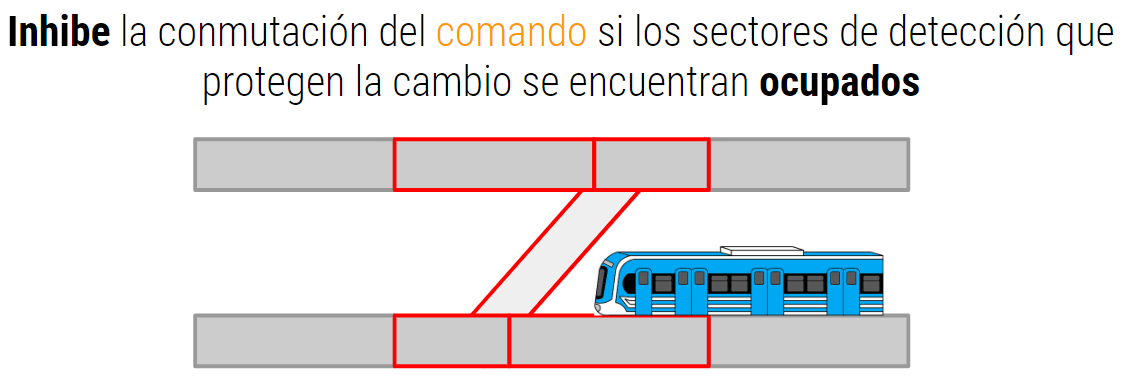
\includegraphics[width=1\textwidth]{Figuras/ocupacion}
        \centering\caption{Bloqueo de máquina de cambios por ocupación de secciones adyacentes.}
        \label{fig:ACG_ocupacion}
    \end{figure}

	La funcionalidad implementada radica en inhibir la conmutación de la máquina de cambios si alguna de las secciones de vías próximas al cambio de vías se encuentra ocupada. De esta manera, se garantiza que la posición del cambio de vías se mantendrá al detectar una formación aproximándose y no se permitirá su conmutación hasta que la formación se encuentre completamente alejada una distancia de seguridad. 
	\subsection{Requerimiento de rutas y bloqueo de cambios en ruta}

\lipsum[1]
    \begin{figure}[!h]
        \centering
        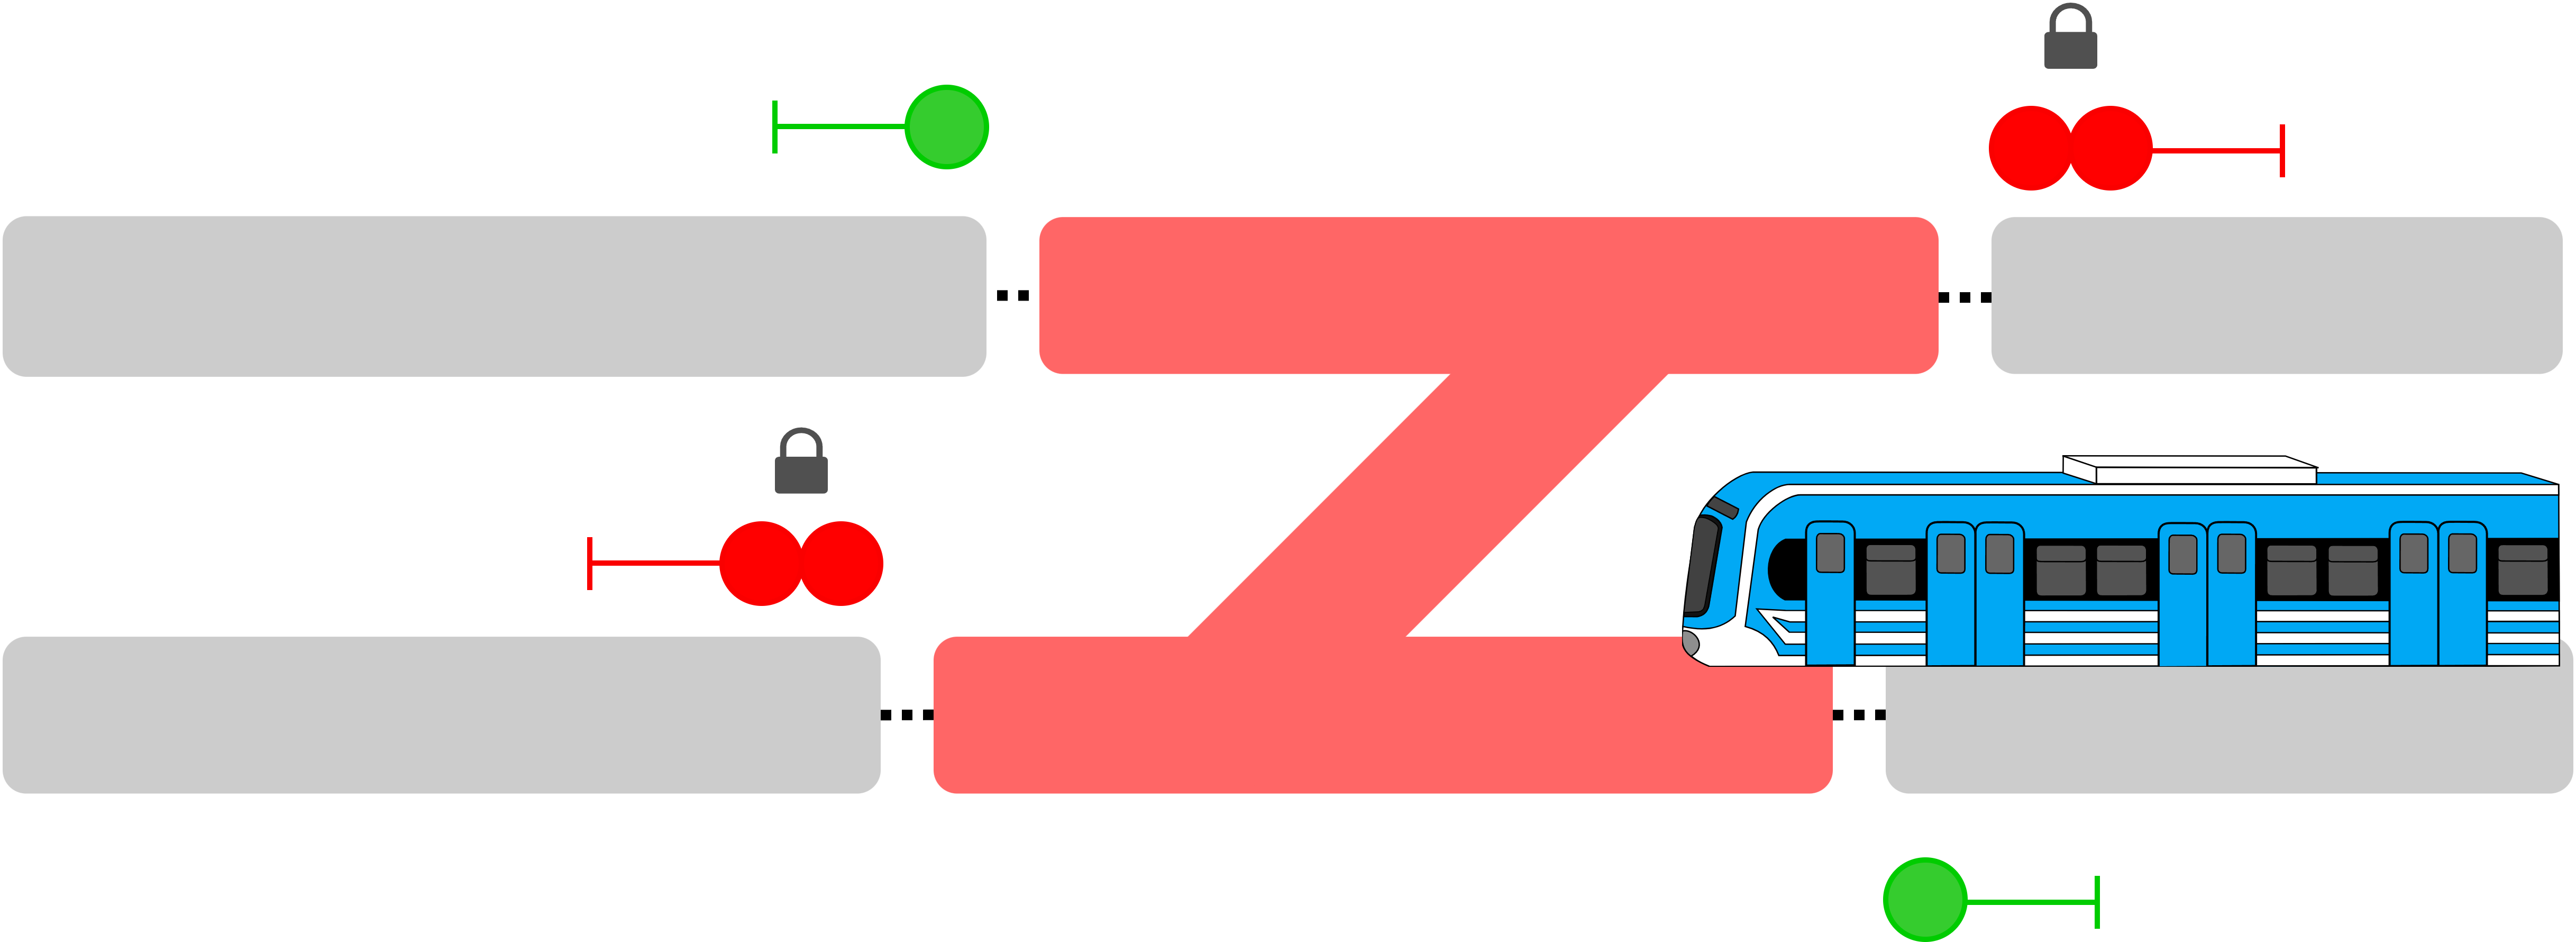
\includegraphics[width=1\textwidth]{Figuras/bloqueo_rutas}
        \centering\caption{XXXXX.}
        \label{fig:ocupacion_1}
    \end{figure}
\lipsum[1]
	\subsection{Protección por aproximación en cancelación de ruta}

	\label{sec:function_3}
	
	La distancia de frenado es un aspecto esencial a considerar cuando una ruta en curso es cancelada. La ruta en cuestión debe seguir protegida durante un tiempo de seguridad.
	
	La Figura \ref{fig:ACG_aproximacion_1} introduce el caso de una formación que tenía una ruta aprobada (aspecto verde) que comenzaba en la sección violeta y abarcaba toda la sección naranja. Por seguridad, ambos cambios de vías fueron bloqueados y sus respectivas señales contrarias fueron forzadas a aspecto rojo y bloqueadas.

    \begin{figure}[!h]
        \centering
        
\includegraphics[width=1\textwidth]{Figuras/aproximacion_1}
        \centering\caption{Formación aproximándose al inicio de la ruta.}
        \label{fig:ACG_aproximacion_1}
    \end{figure}
    
    Mientras la formación se encuentra en movimiento, el operador solicitó la cancelación de la ruta, cambiando el aspecto de la señal a rojo, tal como se visualiza en la Figura \ref{fig:ACG_aproximacion_2}. La formación quizás no tenga el tiempo ni la distancia suficiente para detenerse antes de la señal, por lo que se presentan dos escenarios. 
    
    \begin{figure}[!h]
        \centering
        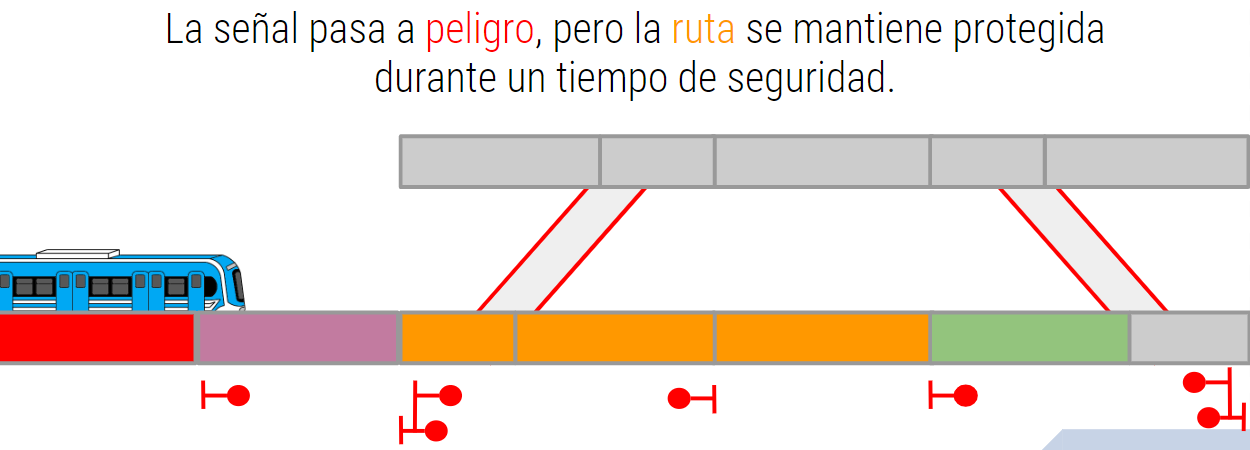
\includegraphics[width=1\textwidth]{Figuras/aproximacion_2}
        \centering\caption{La ruta es cancelada mietnras la formación se aproxima.}
        \label{fig:ACG_aproximacion_2}
    \end{figure}
    
    El primer escenario es el mas favorable: la formación se detiene previo a la señal de peligro y se inicia un contador. Al cumplirse el tiempo de seguridad, las secciones asociadas a la ruta cancelada son liberadas. Lo mismo sucede con los cambios de vías y las señales conflictivas. Este tiempo otorgado permite comprobar que la formación efectivamente se detuvo antes de proceder con la liberación de los elementos ferroviarios para que puedan ser utilizados por otra ruta.
    
    \begin{figure}[!h]
        \centering
        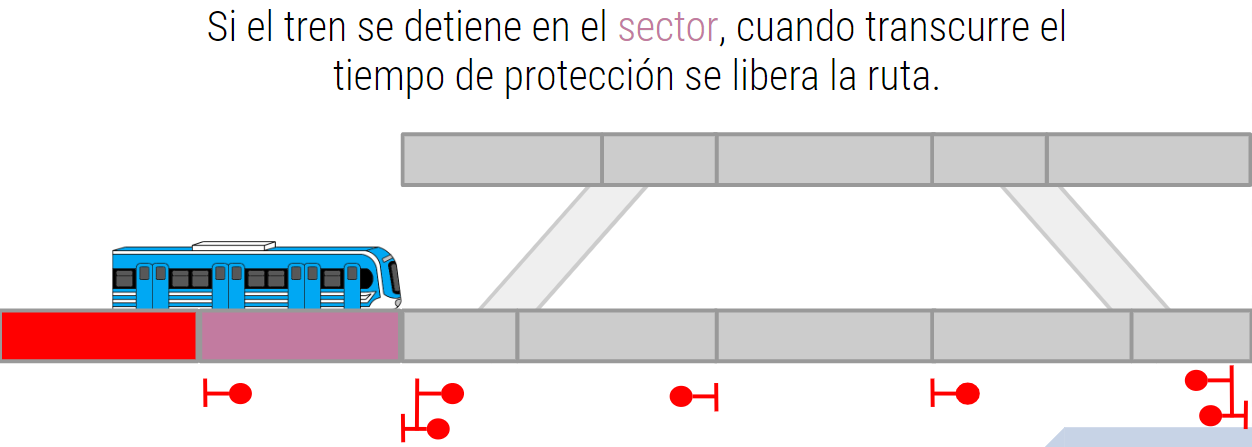
\includegraphics[width=1\textwidth]{Figuras/aproximacion_3}
        \centering\caption{La formación se detiene exitosamente previo a la señal de peligro.}
        \label{fig:ACG_aproximacion_3}
    \end{figure}
    
	En el segundo escenario, la formación no logra detenerse previo a la señal de peligro, tal como se ilustra en la Figura \ref{fig:ACG_aproximacion_4}. Entonces, el sistema de enclavamiento no solamente no libera las secciones pertenecientes a la ruta cancelada, sino que también bloquea las próximas secciones, al no poder estimar cual será la distancia final de frenado de la formación.

    \begin{figure}[!h]
        \centering
        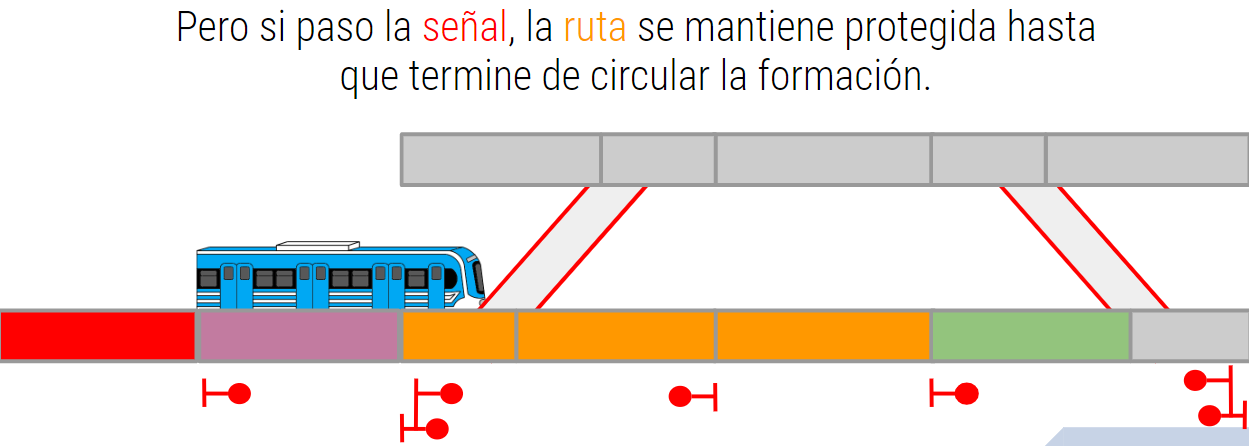
\includegraphics[width=1\textwidth]{Figuras/aproximacion_4}
        \centering\caption{La formación no se detiene previo a la señal de peligro.}
        \label{fig:ACG_aproximacion_4}
    \end{figure}
    
	Las secciones y elementos ferroviarios próximos se mantienen protegidos y enclavados hasta que la ruta se concluya, aún habiendo sido cancelada. Al finalizar la ruta, el sistema de enclavamiento liberará las secciones y elementos ferroviarios próximos al comprobarse que la formación se detuvo previo a la señal de finalización de la ruta.
	
	\subsection{Protección por solape}

	Si una formación no detiene su marcha antes de una señal de peligro, el sistema de enclavamiento debe bloquear las secciones pertenecientes a esa ruta y la próxima, junto con la infraestructura asociado. La Figura \ref{fig:ACG_solape_1} ilustra este suceso, donde una formación ingresa a la sección violeta pasando una señal a peligro, sin tener la autorización requerida. A diferencia de la protección por aproximación, donde una formación no logra detenerse antes de ingresar a una ruta cancelada con poca anticipación, la protección por solape se ocupa de proteger la infraestructura en el caso de que la formación ingrese a una ruta que jamás fue habilitada.

    \begin{figure}[!h]
        \centering
        
\includegraphics[width=1\textwidth]{Figuras/solape}
        \centering\caption{Formación ignora señal a peligro y se activa la protección por solape.}
        \label{fig:ACG_solape_1}
    \end{figure}
    
    Automáticamente, las secciones de la próxima ruta (coloreadas en naranja) son bloqueadas, a la vez que los cambios de vías cercanos y todas las señales tanto consecutivas como contrarias o convergentes. El bloqueo se removerá una vez que la formación se detenga en la próxima señal a peligro, luego de un tiempo de seguridad.
	\subsection{Doble recubrimiento}
	\label{sec:function_5}
	
	Para evitar que una formación colisione con otra formación que se encuentre detenida más adelante en la misma vía o circulando a menor velocidad, el sistema de enclavamiento deberá controlar las señales entre ambas para regular la velocidad y distancia entre ellas. Tal como se explicó en la Sección \ref{sec:signals}, las señales pueden presentar diferentes aspectos. Cada aspecto determinará un rango de velocidad permitido, siendo rojo el mas restrictivo. La Figura \ref{fig:ACG_recrubrimiento_1} ilustra el comportamiento del señalamiento cuando dos formaciones circulan en el mismo sentido, separadas por una distancia de seguridad.
	
	\begin{figure}[!h]
		\centering
		\includegraphics[width=1\textwidth]{Figuras/recubrimiento}
		\centering\caption{Protección por doble recubrimiento.}
		\label{fig:ACG_recrubrimiento_1}
	\end{figure}
	
	La formación que circula por detrás (formación A en la Figura \ref{fig:ACG_recrubrimiento_1}) se encuentra frente a una señal de aspecto verde, por lo
	que puede continuar su marcha sin restricciones, siempre y cuando su velocidad sea menor a la velocidad máxima permitida en la red ferroviaria. Si la formación A reduce la distancia a la formación B, pasará a estar regida por una señal de aspecto amarillo. Si esto sucediera, la formación A deberá disminuir su velocidad para volver a situarse dentro de una sección verde. Lo mismo ocurriría si la formación A alcanzara una señal de aspecto doble amarillo, indicada mediante la señal naranja en la Figura 3.8. En este caso dado que la distancia entre formaciones es aún menor, deberá reducirse aún más la velocidad.
	
	Si la formación A continúa con una mayor velocidad que la formación B, la distancia entre ambas se reducirá y el señalamiento que la formación A tiene en su camino le impondrá velocidades más y más reducidas, hasta que la distancia entre ambas formaciones se incremente a un valor seguro.
		
	Debido al bloqueo por ocupación, todas las secciones ocupadas por una formación presentan una señal a peligro (roja). Inmediatamente detrás de cada formación se genera una secuencia de señales denominada doble recubrimiento. Si la formación avanza y cambia de sección, las señales de protección cambiarán su aspecto acorde al movimiento de la formación, de forma tal que siempre la sección donde está la formación tenga su señal de protección en rojo, la sección anterior en amarillo, la sección anterior en doble amarillo y la sección anterior en verde. Si no hay ninguna formación en la sección anterior a la que tiene su señal en verde, entonces esa sección también tendrá su señal en verde, lo mismo que todas las secciones anteriores, hasta que haya una formación que ocupe una sección, en cuyo caso esa sección estará en rojo y la secuencia de doble recubrimiento se repetirá también detrás de esa formación.
	 
	La cantidad de señales y la secuencia de aspectos variará según el operador de la red, las normas locales o nacionales. Algunos países como el Reino Unido \cite{UK} utilizan la secuencia rojo-doble amarillo-amarillo-verde (Figura \ref{fig:uk_signalling}) y esta es la secuencia de aspectos que implementa el ACG en este trabajo, aunque cabe aclarar que el ACG puede modificarse para implementar otras secuencias. 
	
	\begin{figure}[!h]
		\centering
		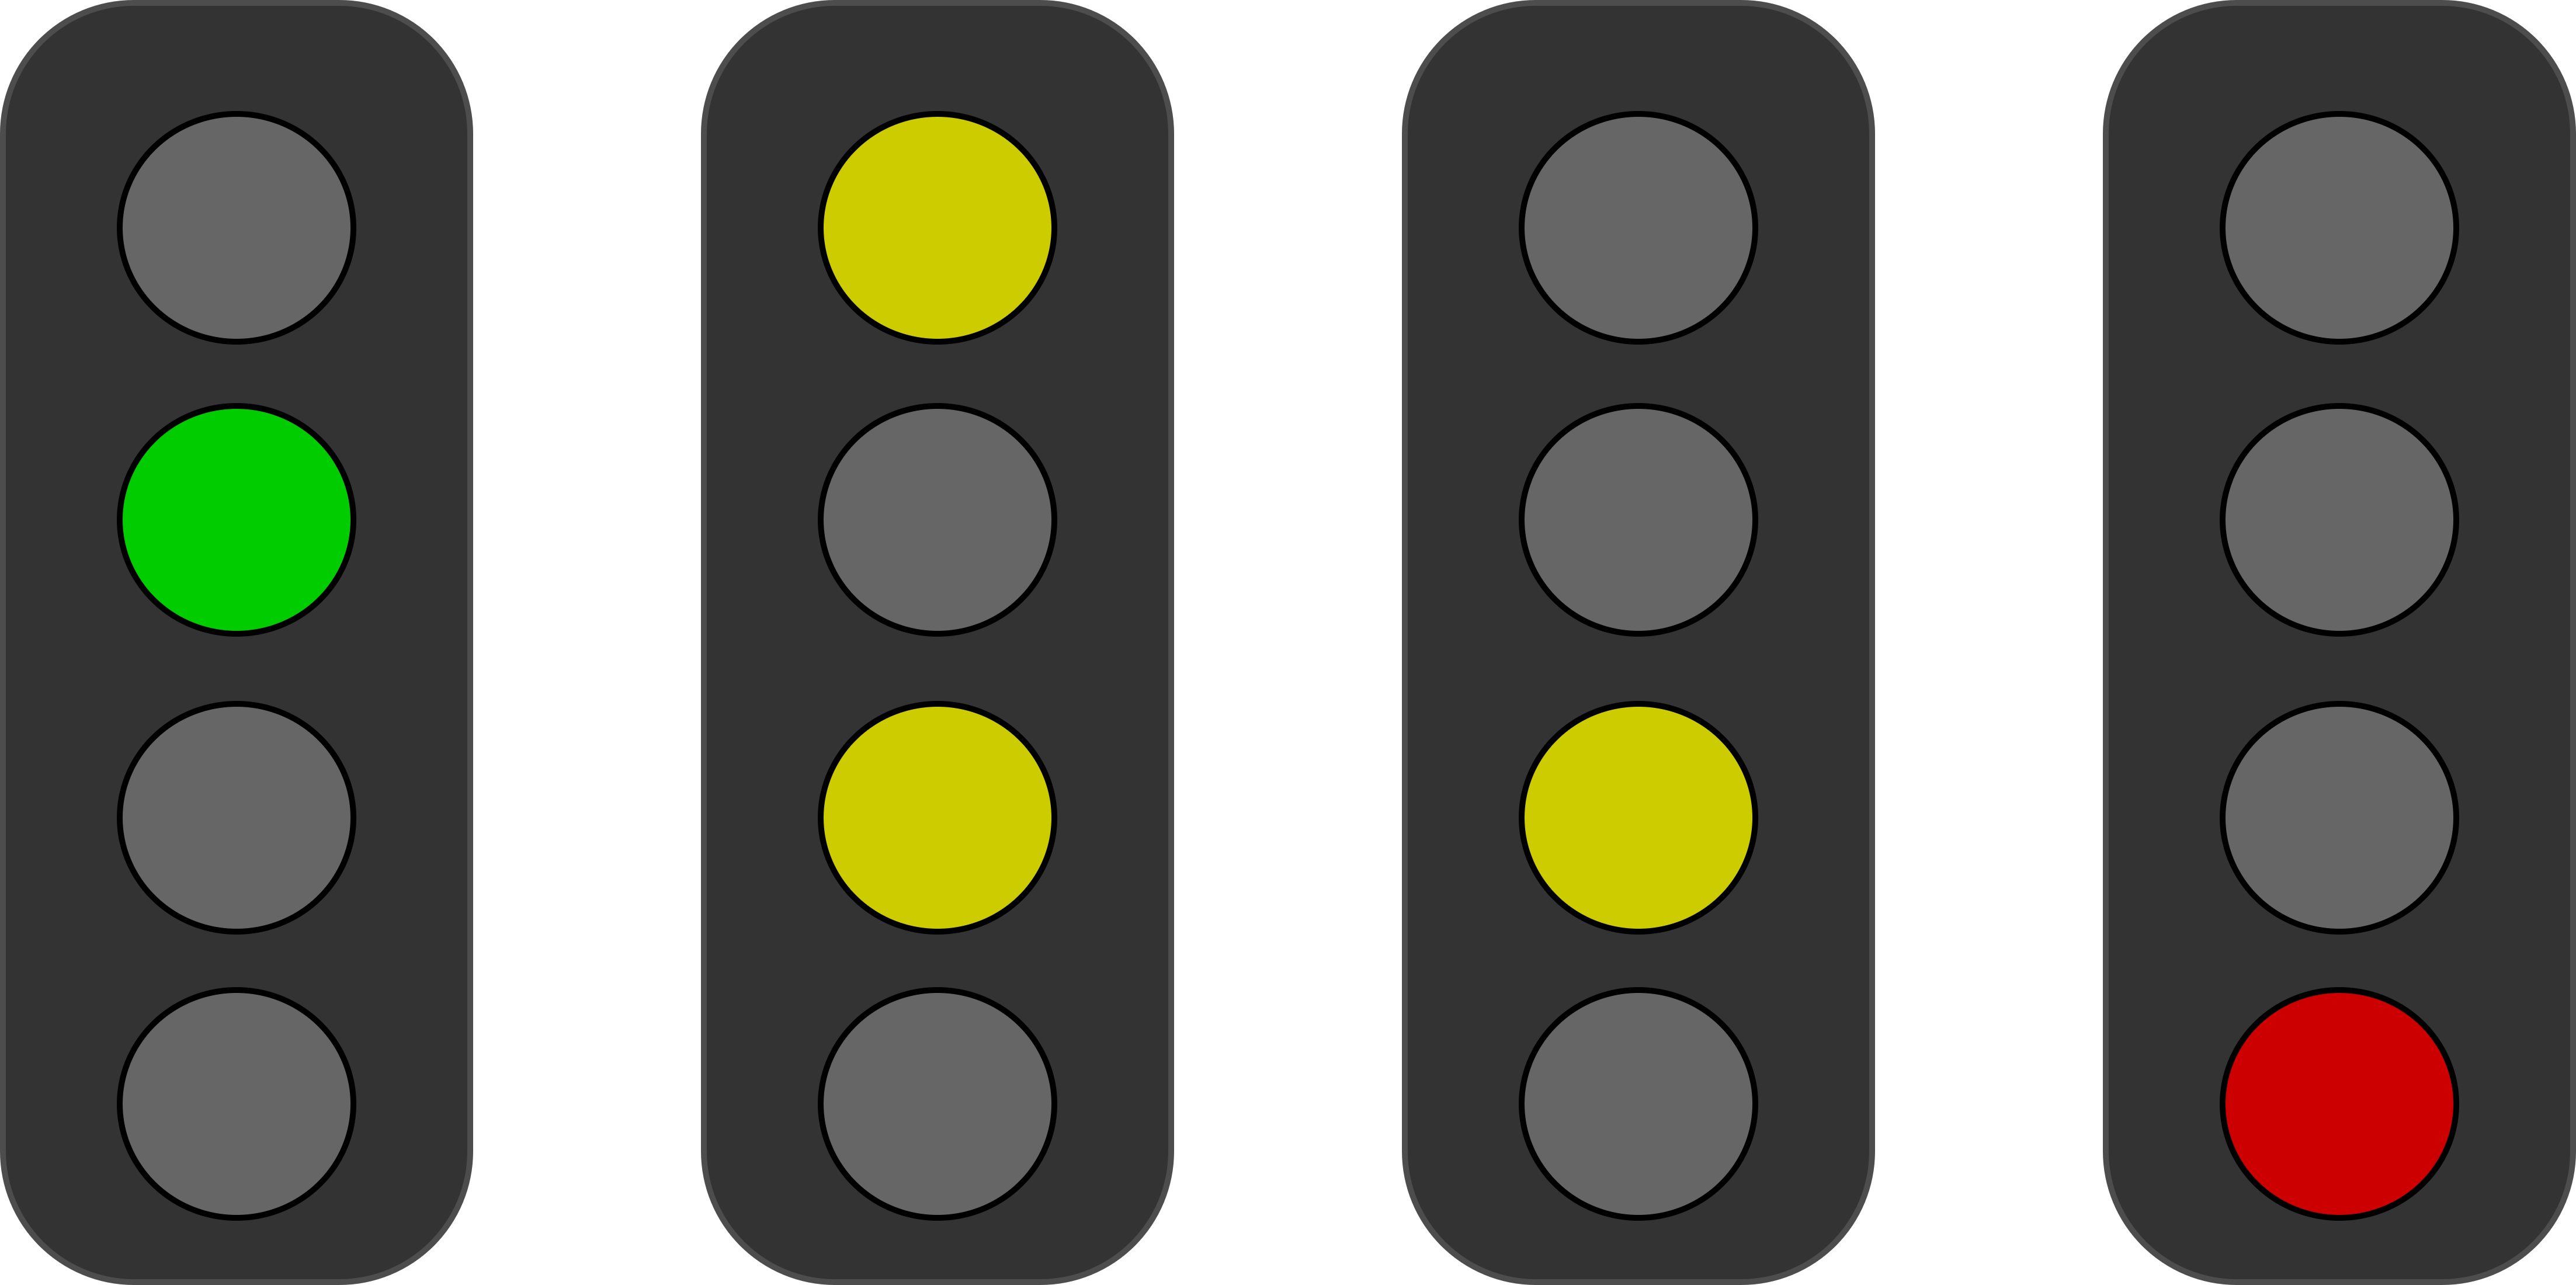
\includegraphics[width=0.5\textwidth]{Figuras/semaforo2}
		\centering\caption{Protección por doble recubrimiento.}
		\label{fig:uk_signalling}
	\end{figure}
	
	En las etapas iniciales del proyecto la única herramienta de visualización era Design4Rail \cite{DESIGN4RAIL}. Esta herramienta solamente puede representar señales de un aspecto y, al no tener todavía implementado el AGG, no era posible representar señales de doble aspecto amarillo. Es por esa razón que el RNA reemplazó la señal doble amarilla por una señal naranja. Este reemplazo también es realizado por el ACG al implementar las señales en VHDL. El proyecto se encontraba en estado muy avanzado cuando se diseñó el AGG, por lo que se mantuvo que todas las señales son de un único aspecto. En este trabajo, por lo tanto, siempre se representará mediante una señal naranja a una señal doble amarilla.
	
	
	%Ya que Design4Rail \cite{DESIGN4RAIL}, el software utilizado para visualizar el señalamiento al inicio del proyecto, solo puede representar señales de un aspecto, en la Figura \ref{fig:ACG_recrubrimiento_1} se reemplazó la señal doble amarilla por una señal naranja. En este trabajo siempre se representará mediante una señal naranja a una señal doble amarilla.

	
	
	\subsection{Liberación secuencial}
	\label{sec:ACG_liberacion}
	
	Esta claro que las rutas conflictivas no pueden ser habilitadas a la vez, pero existen algunas rutas que son parcialmente conflictivas solamente, que comparten una parte de la infraestructura y no toda. La implementación de la liberación secuencial aumenta la flexibilidad en la asignación y habilitación de rutas, mejorando la logística permita por el sistema de enclavamientos. En la Figura \ref{fig:ACG_secuencial_1} se ilustra una formación que iniciará una ruta ya habilitada, para lo cual ya han sido bloqueadas las secciones (coloreadas en naranja) y la infraestructura (coloreadas en rojo).
	
	 \begin{figure}[!h]
	     \centering
	     
\includegraphics[width=1\textwidth]{Figuras/secuencial_1}
	     \centering\caption{Formación iniciando una ruta ferroviaria.}
	     \label{fig:ACG_secuencial_1}
	 \end{figure}
 
	Al ocupar las secciones de vías, debido al bloqueo por ocupación, la señal de inicio de la ruta pasa a peligro y se bloquea la sección consecutiva a la ruta (coloreado en naranja), debido a la protección por solape. Esto se ilustra en la Figura \ref{fig:ACG_secuencial_2}.
	
	\begin{figure}[!h]
    	 \centering
	     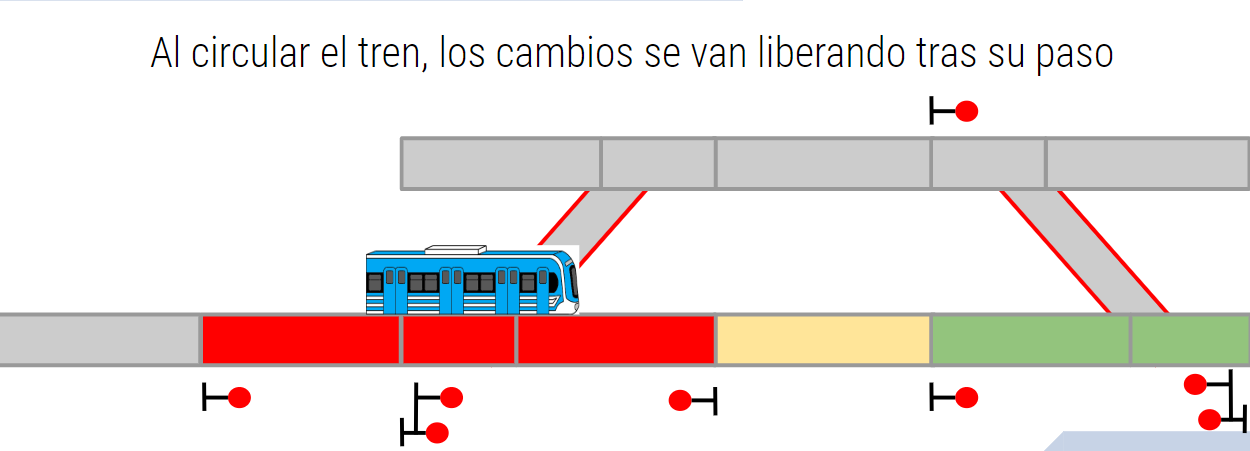
\includegraphics[width=1\textwidth]{Figuras/secuencial_2}
    	 \centering\caption{Formación activando el bloqueo por ocupación y el bloqueo por solape.}
    	 \label{fig:ACG_secuencial_2}
	\end{figure}
 
 	Una vez que la formación desocupa las secciones de vías asociadas al cambio de vías anterior, el sistema de enclavamientos libera inmediatamente toda la infraestructura asociada, como se ilustra en la Figura \ref{fig:ACG_secuencial_3}. A la vez, el sistema de enclavamientos debe esperar a que se cumpla el plazo de seguridad antes de liberar la infraestructura posterior al fin de la ruta. Solamente son liberadas las secciones y señales que ya no son conflictivas.
	   
	\begin{figure}[!h]
	  \centering
	  
\includegraphics[width=1\textwidth]{Figuras/secuencial_3}
	  \centering\caption{Liberación secuencial de la infraestructura por detrás de la formación.}
	  \label{fig:ACG_secuencial_3}
	\end{figure}
 
 	Transcurrido el tiempo de seguridad, el sistema de enclavamientos libera las secciones, cambios de vías, señales y toda infraestructura posterior al fin de la ruta, tal como se ilustra en la Figura \ref{fig:ACG_secuencial_4}.

	 \begin{figure}[!h]
	     \centering
	     
\includegraphics[width=1\textwidth]{Figuras/secuencial_4}
	     \centering\caption{Liberación secuencial de la infraestructura por delante de la formación.}
	     \label{fig:ACG_secuencial_4}
	 \end{figure}
	    
	El ACG implementa estas funcionalidades de seguridad para cada sistema de enclavamientos generado. 
	
	En las siguientes secciones se profundizará en la implementación de cada uno de los módulos del sistema y su comportamiento dinámico. 
    \section{Arquitectura del sistema}

	Cada módulo del sistema fue implementado con máquinas de estado finitas	con camino de datos (FSMD, del inglés Finite State Machine with Data path), que son máquinas de estado finitas (FSM, del inglés Finite State Machine) y circuitos
	secuenciales y combinacionales que constituyen el camino de datos. Utilizar una FSMD aporta un mayor control del diseño a bajo nivel, una mayor portabilidad y un mas eficiente uso de los recursos de la plataforma electrónica.
	
	Una FSMD, cómo la ilustrada en la Figura \ref{fig:FSMD}, posee dos partes diferenciadas: el camino de control y el camino de datos. El camino de control se compone de una FSM que, según las entradas de control y el estado interno que posee, genera señales internas que controlan los circuitos secuenciales del camino de datos. Estos, a su vez, contienen los bloques que procesan las entradas y actúan sobre las salidas.
	
	\begin{figure}[H]
		\centering
		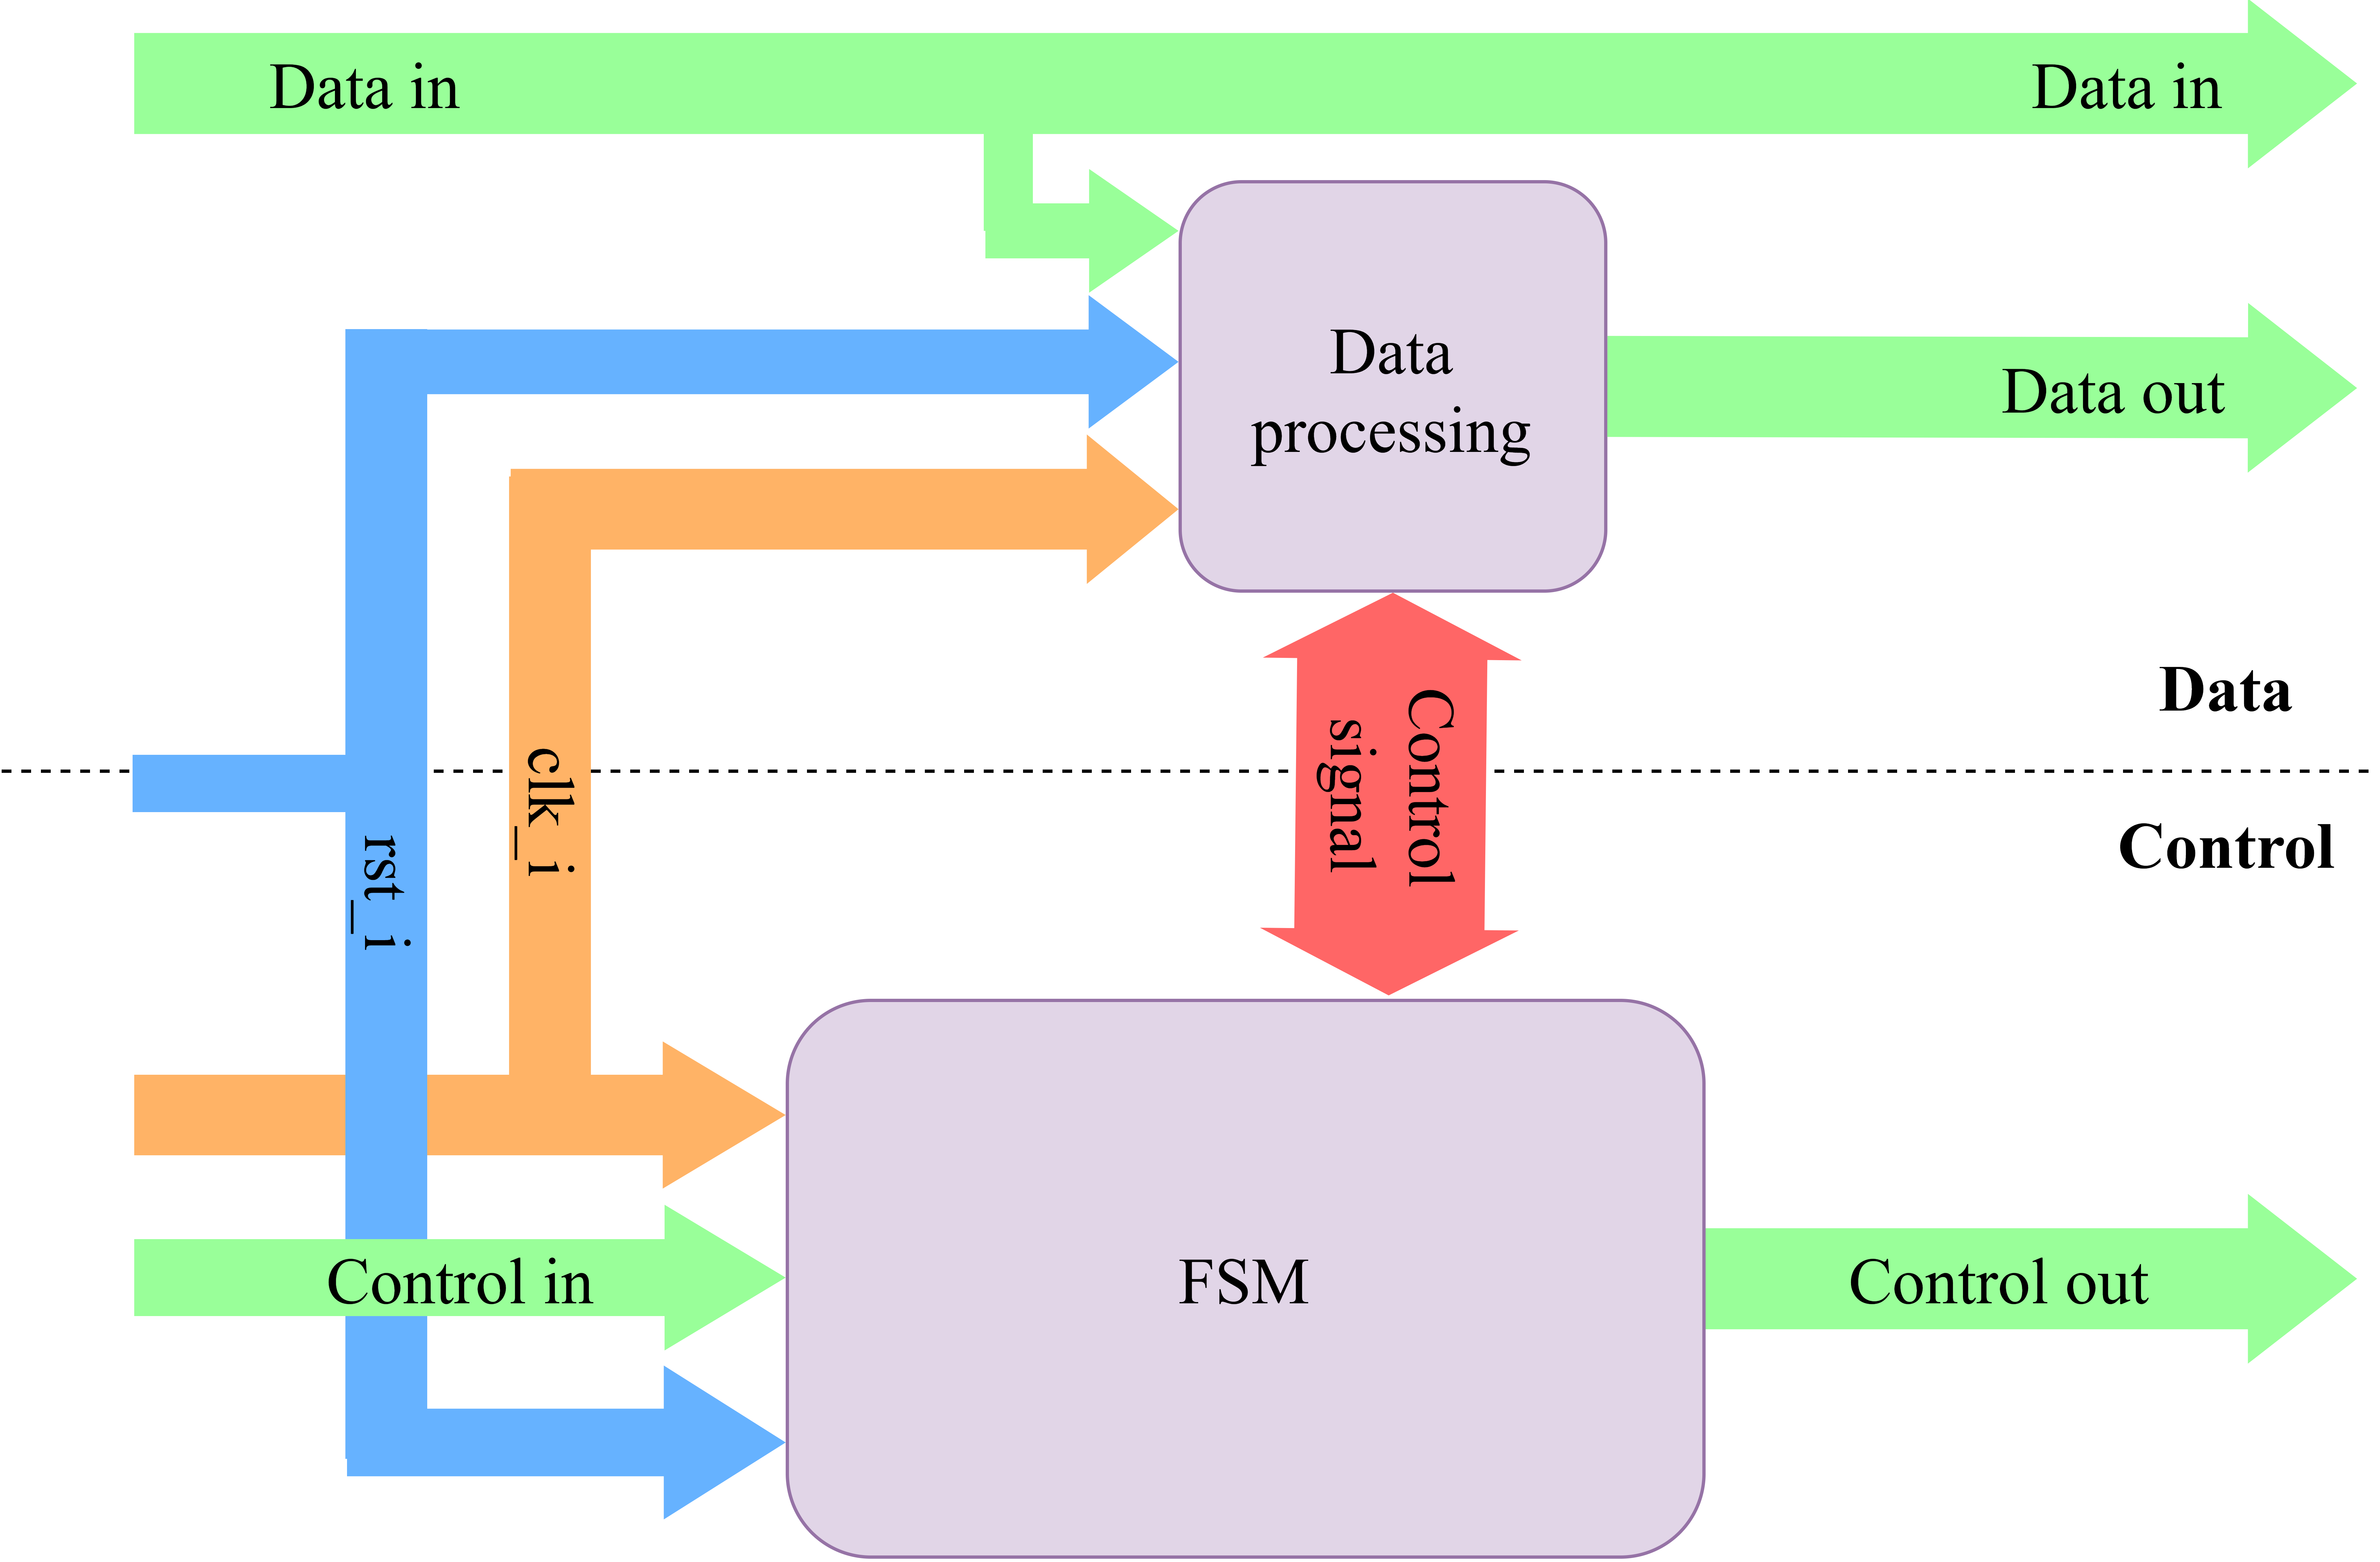
\includegraphics[width=1\textwidth]{Figuras/FSMD.png}
		\centering\caption{Diagrama en bloques  de una FSMD genérica.}
		\label{fig:FSMD}
	\end{figure}
	
	El ACG generará automáticamente cada FSMD en función de los elementos detectados en la red de grafos. Es decir, el modelado de cada elemento será una plantilla que contemplará todos los casos posibles, con todas las entradas y salidas posibles, pero solo se implementarán las funcionalidades que cada elemento particular requieran. De esta manera, será posible optimizar los recursos a la vez que se valida cada elemento una única vez, como un objeto genérico.
	
	Los elementos ferroviarios a ser modelados por el ACG son los que denominaremos elementos dinámicos. Es decir, todo elemento ferroviario que posea algún estado susceptible de modificarse en función de algún evento o del tiempo. Estos elementos dinámicos pueden adoptar los siguientes estados:
	
	\begin{itemize}
		\item Circuitos de vía: ocupados, desocupados.
		\item Rutas: no solicitadas, solicitadas.
		\item Señales: rojo, doble amarillo, amarillo, verde
		\item Pasos a nivel: barrera baja, barrera alta.
		\item Cambios de vías simples: posición normal, posición reversa.
		\item Cambios de vías dobles: posición doble normal, posición doble reversa, posición normal reversa, posición reversa normal.
		\item Cambios de vias en tijeras: posición normal, posición reversa.
	\end{itemize}
	
	Internamente, el sistema contemplará que algunos elementos pueden admitir estados de transición. Estos estados son producto del tiempo que requiere un actuador para completar las comandos que la FPGA envía. No obstante, los estados de transición solo serán tolerados un tiempo determinado, pasado el cuál se asumirá que la orden no fue completada y se abortará la ejecución de la ruta solicitada.
	
	La arquitectura general del sistema generado por el ACG se ilustra en la Figura \ref{fig:GeneralSystem}. El módulo \textit{Detector} recibe las tramas en formato serie, comprueba su integridad y en caso de que los datos contengan solamente caracteres válidos los entrega al módulo \textit{Decoder}. El módulo \textit{Decoder} toma esos datos y los paraleliza para entregarlos al módulo \textit{Network} en la entrada que corresponda a cada dato. El módulo \textit{Network} es la implementación de la red de grafos generada por el RNA. 
	
	\begin{figure}[H]
		\centering
		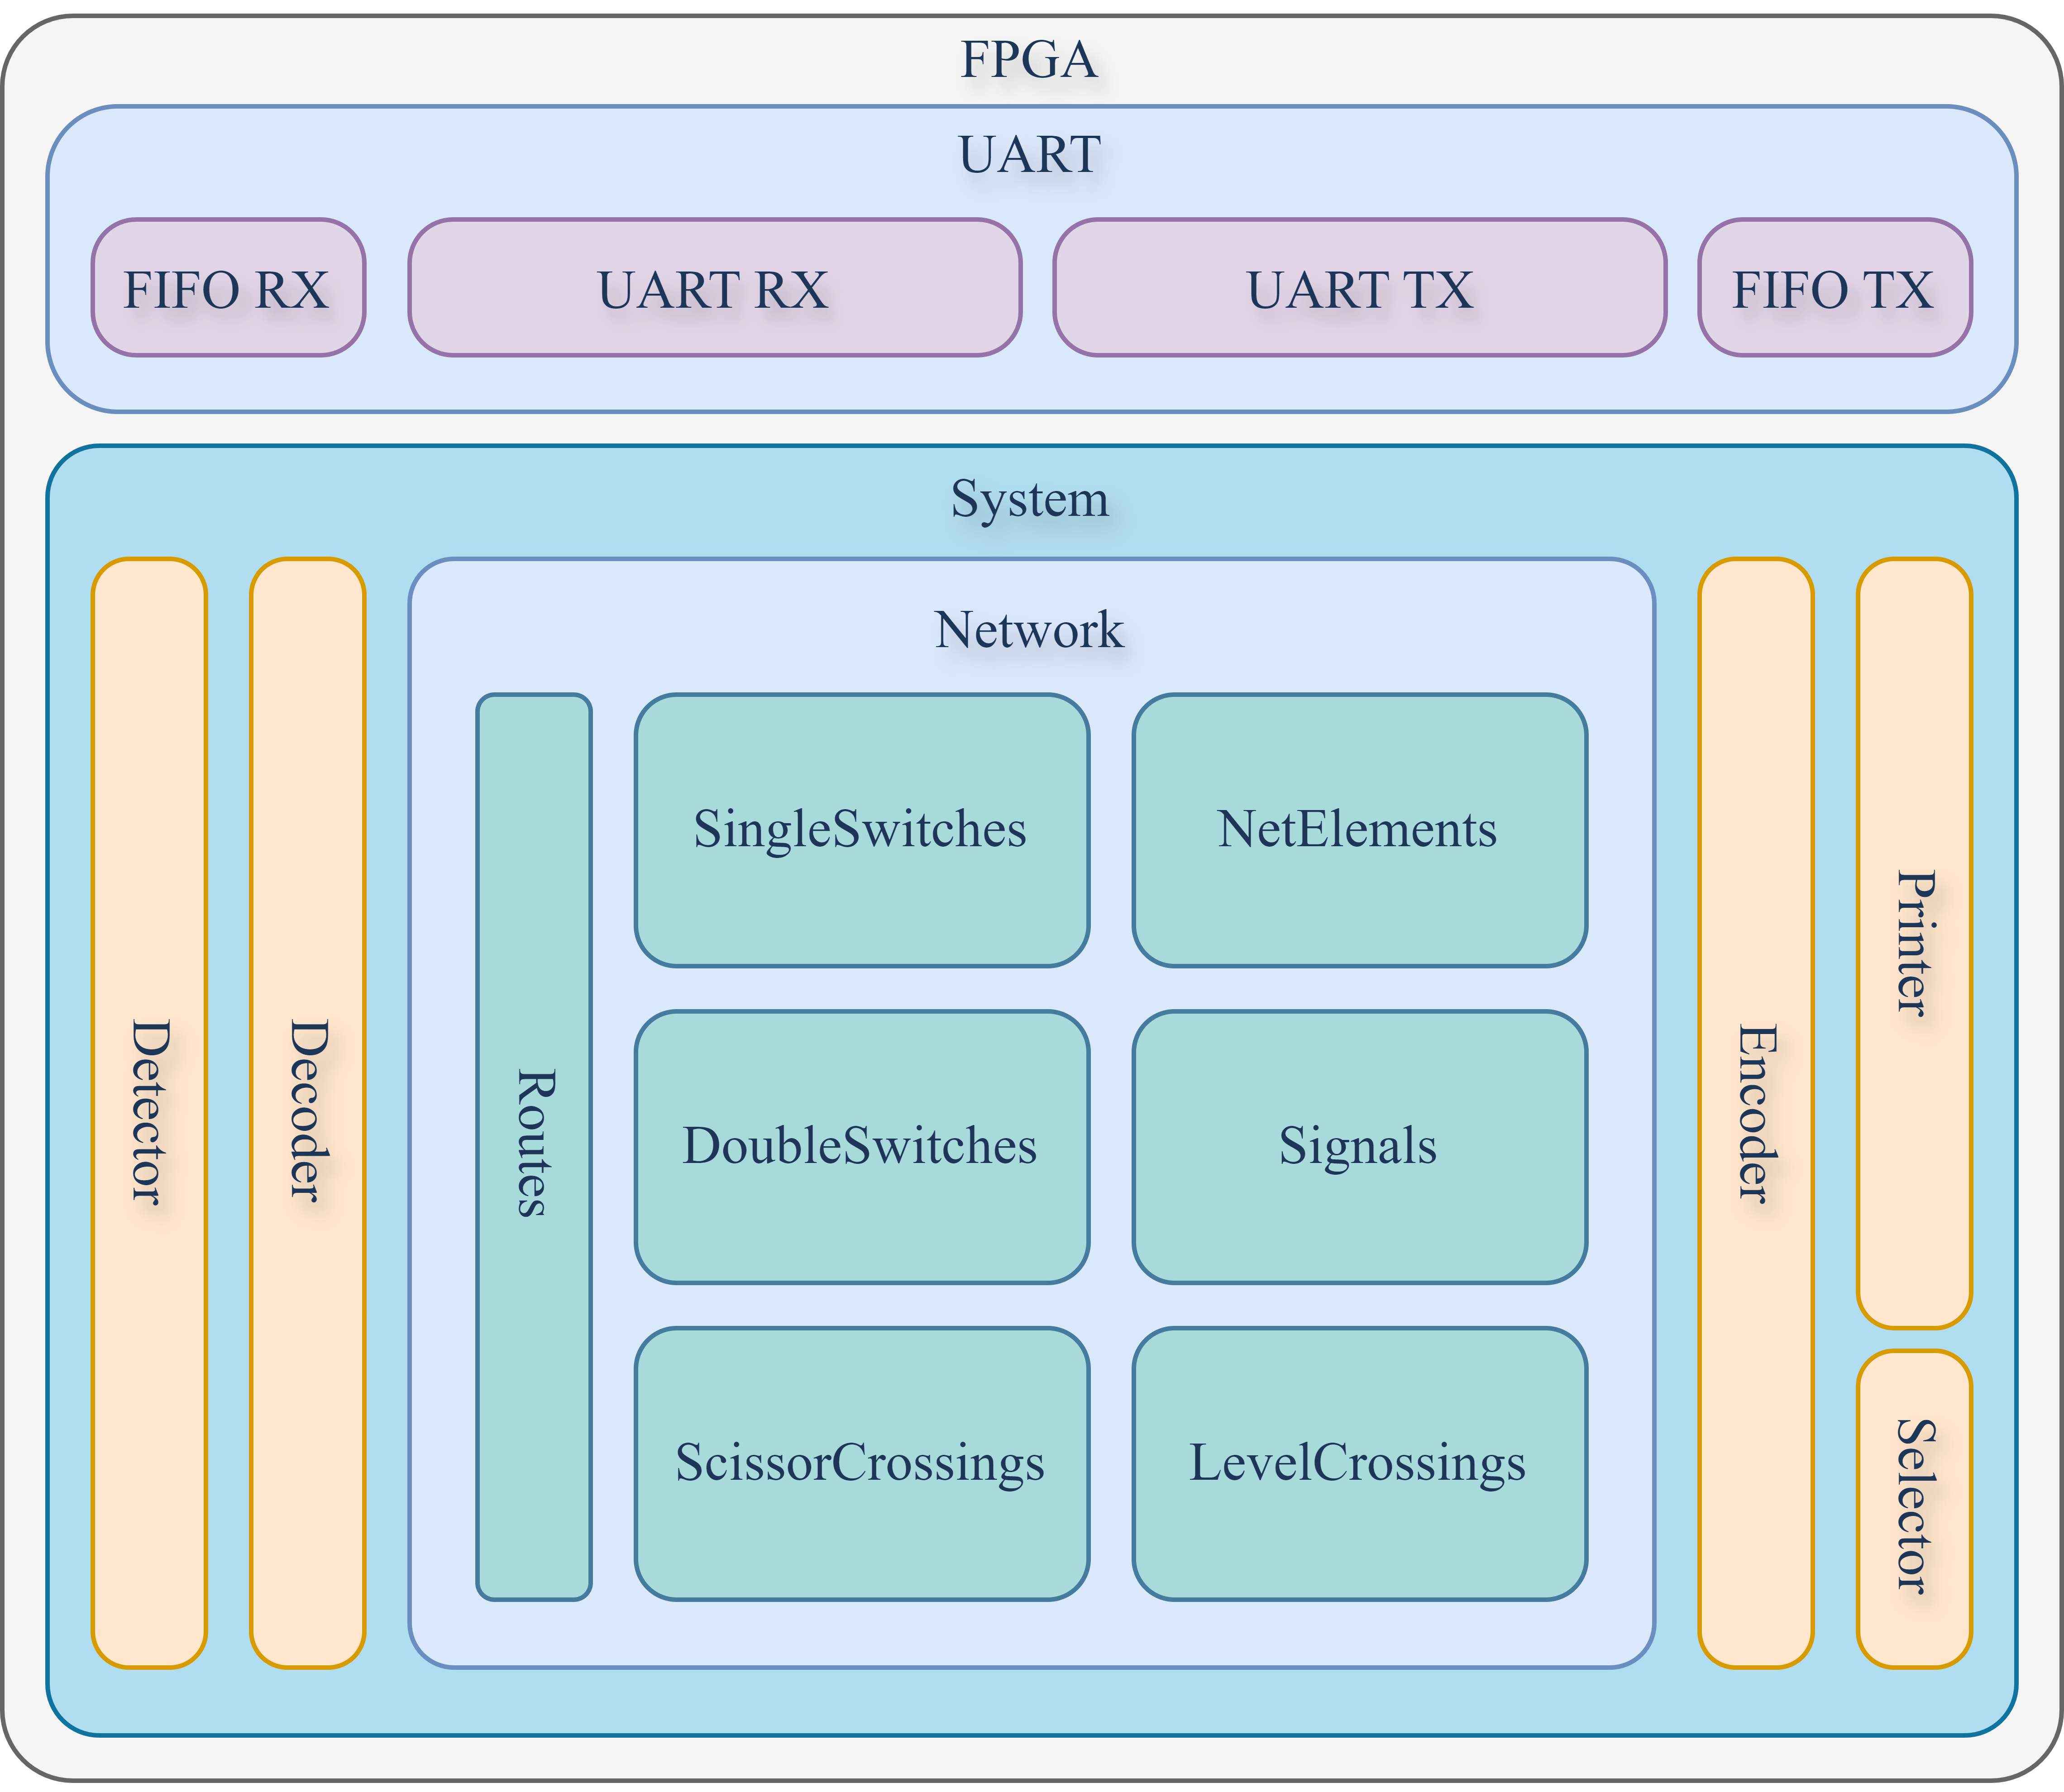
\includegraphics[width=1\textwidth]{Figuras/Arq_general.png}
		\centering\caption{Arquitectura general del sistema generado por el ACG.}
		\label{fig:GeneralSystem}
	\end{figure}
	
	El módulo \textit{Encoder} toma las salidas generadas por el módulo \textit{Network}, las agrupa apropiadamente y se las suministra al módulo] \textit{Printer}. El módulo \textit{Printer} transforma cada elemento de la señal en un caracter imprimible para enviar a la UART. Finalmente, el módulo \textit{Selector} se usa exclusivamente a los fines de comprobar el correcto funcionamiento de la comunicación serie, puenteando a todos los otros módulos.
	
	La descripción del sistema se realizará desde sus módulos mas externos, que implementan la comunicación del sistema: los módulos de UART, Detector, Decoder, Encoder y Printer. De forma tal de entender en alto nivel como es el proceso de comunicación hacia y desde la FPGA, para luego abordar el núcleo del sistema de enclavamiento. cuya complejidad es mucho mayor.		
	
	\subsection{Modulo UART}
\label{sec:UART}
	Si consideramos la lista de elementos dinámicos y cada estado que pueden admitir, es claro que la cantidad de señales sobrepasaría por mucho la limitada cantidad de puertos que una FPGA pueda proveer. Por ejemplo, si se considera un sistema ferroviario como el presentado en la Figura \ref{fig:bypass_1}, que por comodidad para el lector se copia en la Figura \ref{fig:bypass_3}, seria necesario mas de 25 pines de la FPGA entre entradas y salidas, lo que implicaría que para ese sistema tan simple se requeriría utilizar una FPGA de tamaño medio o grande. Esto implica que ese enfoque dificultaría la implementación del sistema de enclavamiento de redes ferroviarias de mayor tamaño.
	
	\begin{figure}[H]
		\centering
		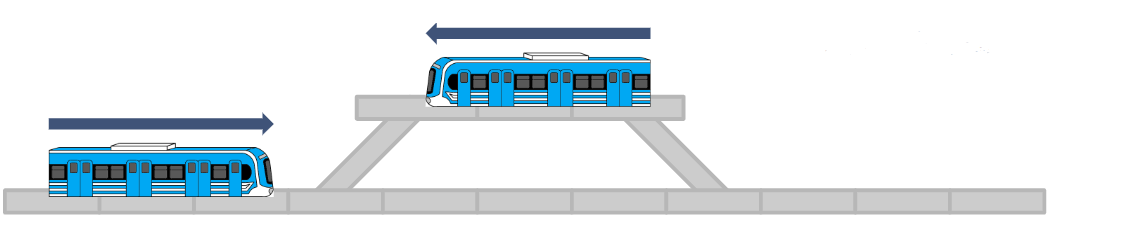
\includegraphics[width=1\textwidth]{Figuras/bypass}
		\centering\caption{Topología de derivación ferroviaria.}
		\label{fig:bypass_3}
	\end{figure}
	
	Es por eso que se decidió que la FPGA mediante la cual se implemente el sistema de enclavamiento debe recibir y transmitir la información a la cabina de señalamiento en formato serie. El uso de comunicación serie para la implementación del sistema es apropiado, ya que otros sistemas ferroviarios utilizan comunicación serie, como por ejemplo RS-485 o MVB en las redes de comunicación de trenes (TCN, del inglés \textit{Train Communication Network}) \cite{TCN}. La comunicación a implementar entre el sistema de enclavamiento y la cabina de señalamiento deberá ser flexible para ser utilizada en diferentes implementaciones con menor o mayor cantidad de elementos ferroviarios.
	
	En la Figura \ref{fig:GeneralCom} se presenta la propuesta de conexión de la FPGA con una computadora externa, que para el desarrollo y prueba de la solución hará las veces de la cabina de señalamiento. En la Figura \ref{fig:GeneralCom} también se representan los módulos internos de comunicación. La UART (del inglés \textit{Universal Asynchronous Receiver-Transmitter}), junto con las memorias FIFO (del inglés \textit{First-In First-Out}), se utilizan para implementar el intercambio de las tramas de datos entre la FPGA y la computadora.
	
	\begin{figure}[H]
		\centering
		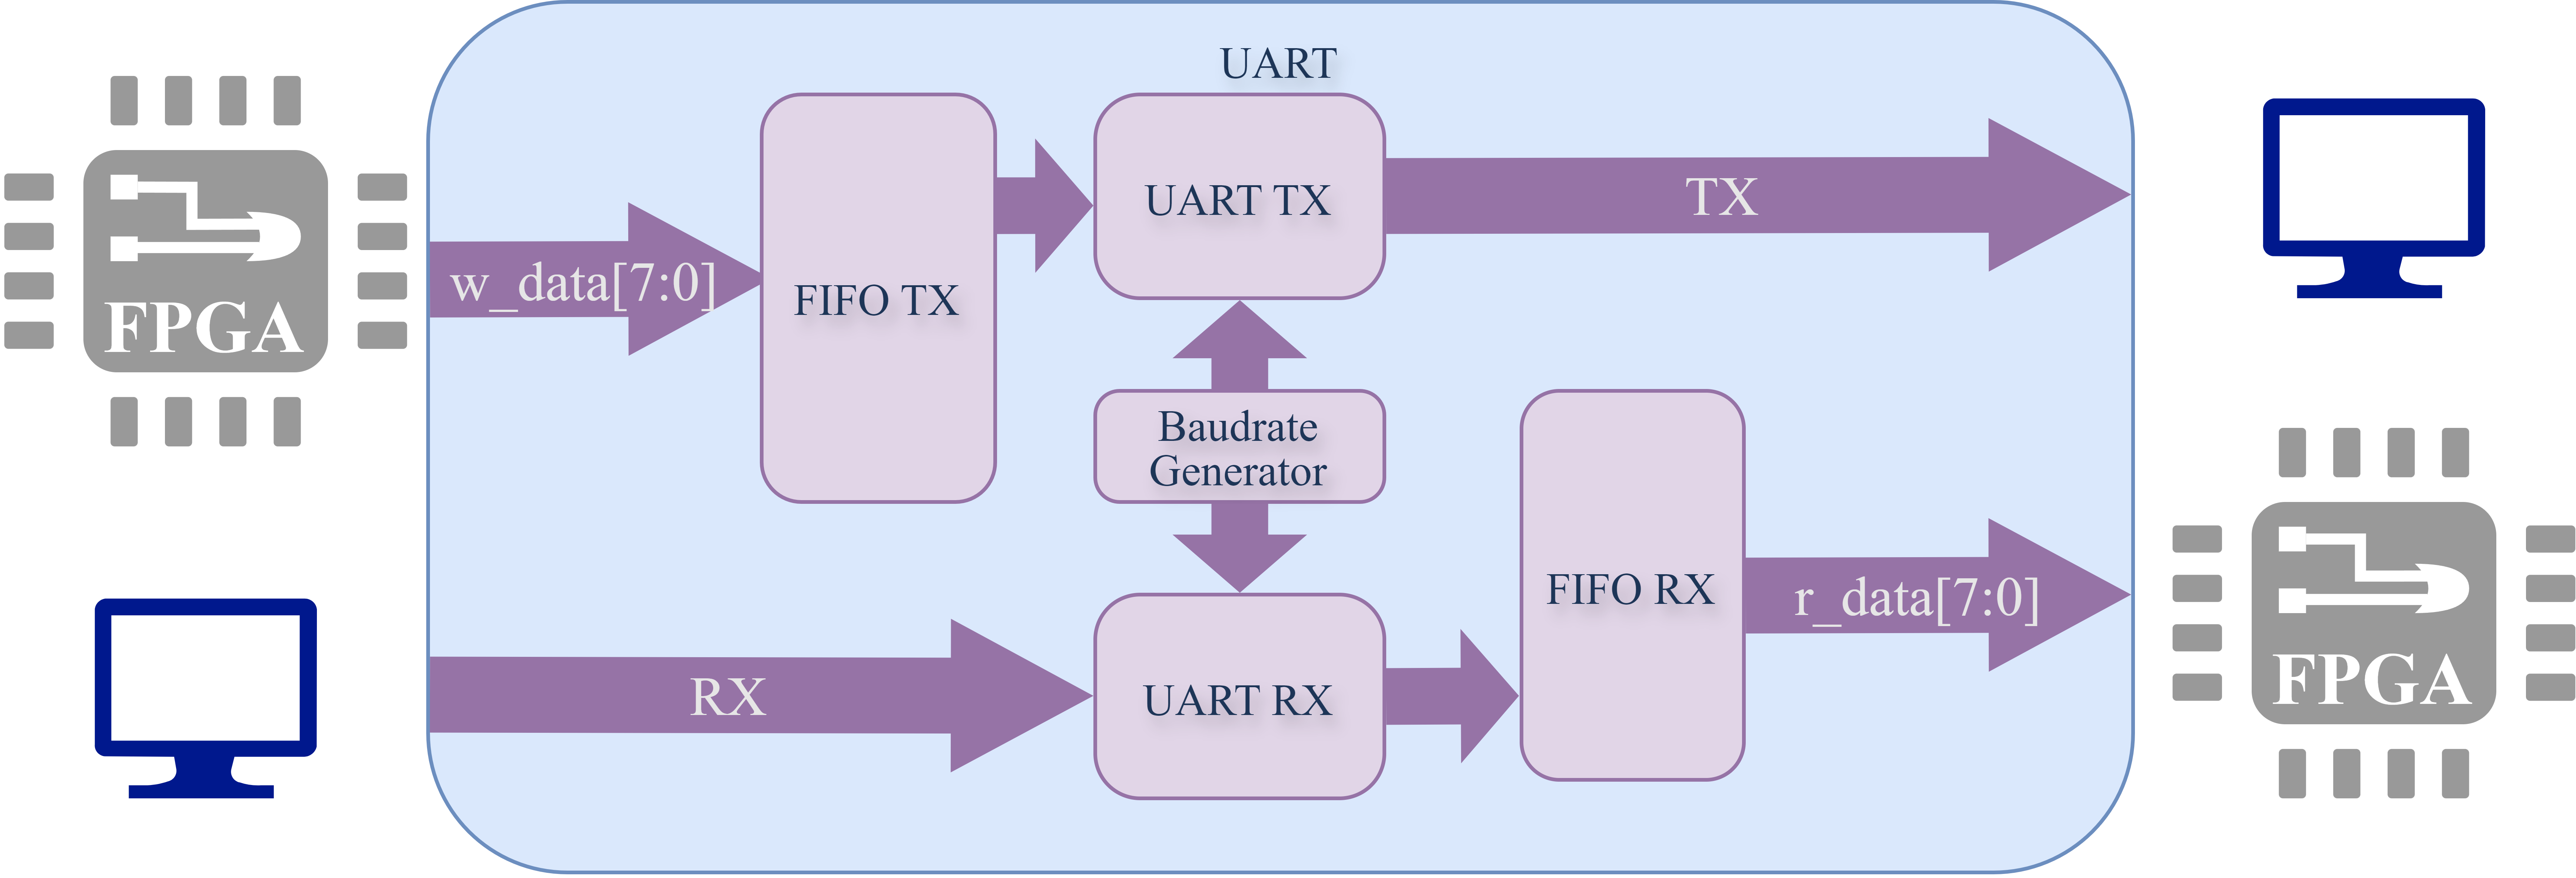
\includegraphics[width=0.7\textwidth]{Figuras/UART_module.png}
		\centering\caption{Conexión entre la FPGA y una computadora externa.}
		\label{fig:GeneralCom}
	\end{figure}
	
	El módulo de recepción (UART RX), que se ilustra en la Figura \ref{fig:GeneralCom}, es el encargado de procesar cada bit recibido con un baudrate preestablecido y almacenar cada bit en la FIFO RX. Al completarse un byte de datos, será enviado al sistema de enclavamientos, junto con una serie de pulsos para indicar cuándo deben ser leídos. El sistema de enclavamientos esperará a tener la cantidad de bytes necesarios (definidos por el ACG) para empezar a procesar la trama. Luego, el sistema de enclavamientos devolverá una nueva trama de bytes a la FIFO TX. Finalmente la nueva trama será enviada al módulo de transmisión (UART TX) que enviará la información bit a bit, con el mismo baudrate que fue recibido.
	
	La implementación de los módulos de transmisión y recepción de la UART es invariante para cada locación, es decir, los recursos asignados serán los mismos, cualquiera sea el tamaño del sistema a implementar. Los módulos de memorias FIFO, en cambio, dependen de las características y del tamaño del sistema. Locaciones mas complejas tendrán valores de N y M mayores y, por lo tanto, requerirán FIFOs mas grandes. 
	
	En la Figura \ref{fig:Stream} se ilustra el formato definido para las tramas de entrada y salida. La trama tendrá un tamaño de entrada N y de salida M, con N igual que M. La cantidad de cada elemento ferroviario es definida por el RNA y el orden de los elementos es fijo y definido en el ACG. Los elementos que no existan en la locación analizada tendrán paquetes de datos de largo nulo. Además, la trama tendrá un caracter delimitador de entrada y de salida ($<$ y $>$ respectivamente). Todos los elementos de la trama serán hexadecimales en formato ASCII, para poder ser interpretados fácilmente en una terminal y ser menos susceptibles a errores por alteraciones en algún bit aleatorio.
	
	\begin{figure}[H]
		\centering
		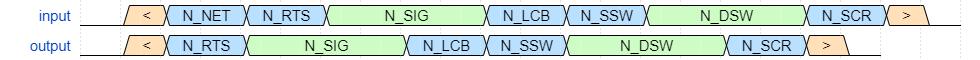
\includegraphics[width=1\textwidth]{Figuras/Tramas.png}
		\centering\caption{Tramas de datos y paquete de datos.}
		\label{fig:Stream}
	\end{figure}
	
	El largo de la trama de entrada y de salida queda definido por la Ecuación \ref{eq:StreamLength_in}. 
	
	\begin{equation} 
		\label{eq:StreamLength_in}
		\text{N} = 1\text{byte} (\text{N}_{NET}+\text{N}_{\text{RTS}}+\text{N}_{\text{LCB}}+\text{N}_{\text{SSW}}+\text{N}_{\text{SCR}}\text{N}_{\text{SIG}}+\text{N}_{\text{DSW}})
	\end{equation}
	
	Cada elemento dinámico requiere un sólo caractér hexadecimal para definir su estado utilizando sus 4 bits. Los 2 bits menos significativos definen el estado (\textit{STATE} en Figura \ref{fig:Stream}). Por ejemplo, la posición de un cambio de vías o el aspecto de una señal. Los 2 bits mas significativos definen el enclavamiento del elemento dinámico (\textit{LOCK} en la Figura \ref{fig:Stream}). El parámetro \textit{Lock} puede tomar tres valores: '00' para elementos disponibles, '01' para elementos que han sido reservados por una ruta pero aún no han sido enclavados y '10' para elementos enclavados.
	
	En la Figura \ref{fig:Stream_ejemplo1} se ilustran dos tramas recibidas en el caso de una topología ferroviaria que será explicada en profundidad en la Sección \ref{sec:ejemplo_1}, y que a modo de referencia se presenta en la Figura \ref{fig:EJ1_2_B}. La primer trama de datos representa el estado del sistema de enclavamiento cuando no se han solicitado rutas y la segunda ilustra una ruta pedida y habilitada. Ambas tramas corresponden a la misma topología ferroviaria y cuentan con 11 netElements, 21 rutas, 23 señales, 2 pasos a nivel, 5 cambios de vías y los correspondientes tags iniciales y finales.
	
	\begin{figure}[H]
		\centering
		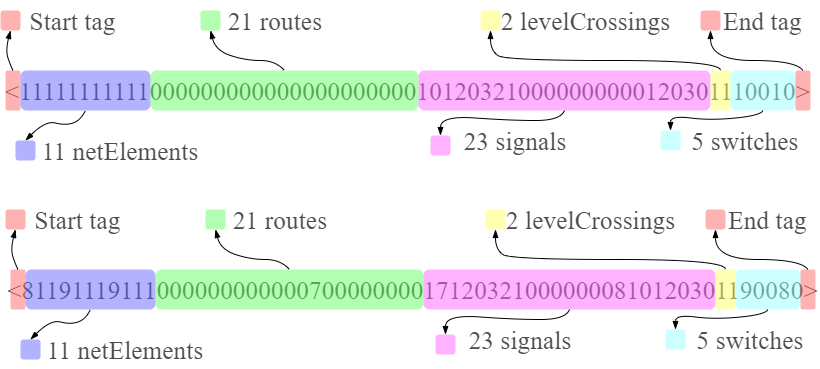
\includegraphics[width=1\textwidth]{Figuras/Trama_ejemplo.png}
		\centering\caption{Tramas de datos y paquete de datos.}
		\label{fig:Stream_ejemplo1}
	\end{figure}
	
	En la primer trama se pueden apreciar: 11 secciones de vías sin ocupar (todos los valores en 1), 21 rutas sin solicitar (todos los valores en 0), 23 señales de las cuales podemos destacar 14 señales rojas (valores en 0), 4 señales naranjas (valores en 1), 3 señales amarillas (valores en 2) y 2 señales verdes (valores en 3). Además, la trama describe dos pasos a nivel con el brazo de barrera en alto (todos los valores en 1) y 5 cambios de vías, 3 de ellos en posición normal (valores en 0) y 2 en posición reversa (valores en 1). Debido que no existen rutas solicitadas ni habilitadas en esta trama (todos los valores en 0), todos los elementos tienen sus valores de LOCK en '00', lo que indica que se encuentran disponibles para ser enclavados por la ruta correspondiente.

	En la segunda trama, en cambio, se puede apreciar que el primer netElement (ne1) es representado con un 8 (1000), lo cual significa que se encuentra enclavado (10) y ocupado (00). Los netElements ne9 y ne15 son representados con un 9 (1001), ya que también se encuentran enclavados (10), pero no han sido ocupados (01). Además, la ruta 12 es representada con un 7 (0111), el estado de liberación secuencial (que será explicado en la Sección \ref{sec:ACG_rts}). Los semáforos que presentan valores superiores a 4 (0100) son aquellos que se encuentran reservados y los que presentan valores superiores a 8 (1000) se encuentran enclavados. En este caso, el semáforo S22 se representa con un 7 (0111, verde y reservado) y el semáforo T05 se representa con un 8 (1000, rojo y enclavado). Finalmente, los cambios de vías pares se encuentran en posición normal y los impares en posición reversa. En el caso del cambio de vías sw04, el valor 9 representa un cambio de vías enclavado en posición reversa y el cambio de vías sw07, el valor 8 representa un cambio de vías enclavado en posición normal.
	
	\begin{figure}[H]
		\centering
		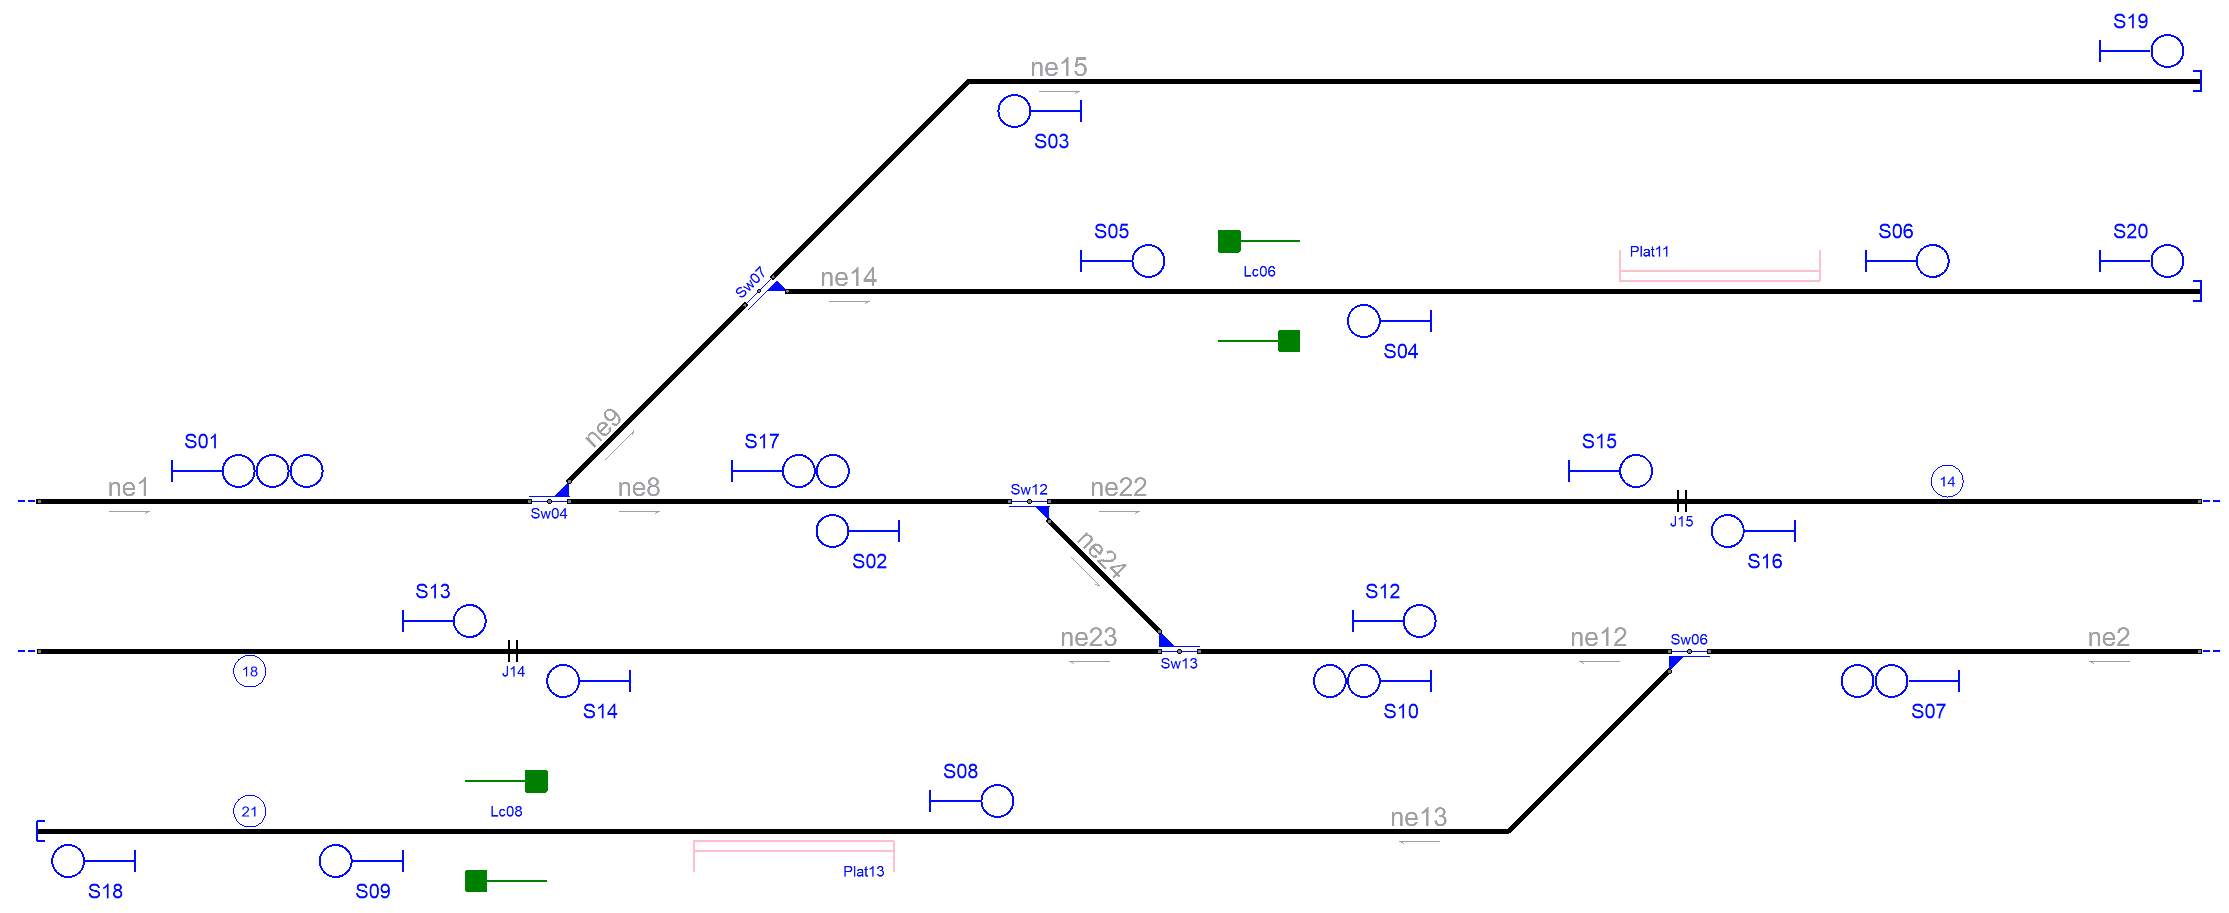
\includegraphics[width=1\textwidth]{resultados-obtenidos/ejemplo1/images/1_original.png}
		\centering\caption{Topología ferroviaria del ejemplo 1.}
		\label{fig:EJ1_2_B}
	\end{figure}
	
	
	
	
	
	
	%11111111111000000000000000000000101203210000000000120301110010
    %81191119111000000000000700000000171203210000000810120301190080
	
	
	%Con este criterio de diseño, en todos los demás casos, la FIFO de salida tendrá el mismo tamaño que la FIFO de entrada o a lo sumo será 50 \% menor, lo que representa un ahorro de 25 \% de los recursos estimados. Por ejemplo, si se necesita que la entrada tenga 15 bits y la salida 7 bits y se le asignara el mismo tamaño a ambas FIFOs; tanto la FIFO de entrada como la de salida necesitarán 16 bits cada una, dando un total de 32 bits. Pero si se aplica el criterio de tamaños desacoplados, entonces para la FIFO de salida podrían asignarse solamente 8 bits, dando un total de 24 bits, un 25 \% menos que los 32 bits que necesitaría si ambas FIFOs quedaran definidas según los datos de la entrada.
	\subsection{Módulo Detector}
	\label{sec:detector}
	
	El módulo \textit{detector} es el encargado de detectar el inicio y final de cada trama, validando que el contenido de la misma tenga N caracteres, conforme al formato de trama expuesto en la Sección \ref{sec:UART}. A medida que la validación tiene lugar, los caracteres ASCII son convertidos en valores booleanos (\textit{std\_logic}) dentro de un vector de elementos booleanos llamado \textit{packet}[N] (\textit{std\_logic\_vector} de N elementos). El diagrama de bloques de las máquinas de estado finitas con camino de datos se muestra en la Figura \ref{fig:Detector_module}.
	
	\begin{figure}[H]
		\centering
		\includegraphics[width=1\textwidth]{Figuras/Detector_module.png}
		\centering\caption{FSMD del módulo \textit{Detector}.}
		\label{fig:Detector_module}
	\end{figure}
	
	En cada pulso de reloj (\textit{clk\_i}), el módulo UART envía un caracter por medio de la señal \textit{r\_data} (8 bytes) y un pulso (\textit{r\_available}) para informar que un nuevo dato ha sido enviado. El pulso de reloj es utilizado principalmente en el módulo \textit{Counter\_0\_to\_N}, cuyo parámetro N ya ha sido calculado por el ACG previo a generar el código y es la cantidad de caracteres que serán enviados a continuación del caracter de inicio. El proceso de detección y validación de la trama recibida se describe el diagrama de estados de la Figura \ref{fig:Detector_FSMD}.
	
	\begin{figure}[H]
		\centering
		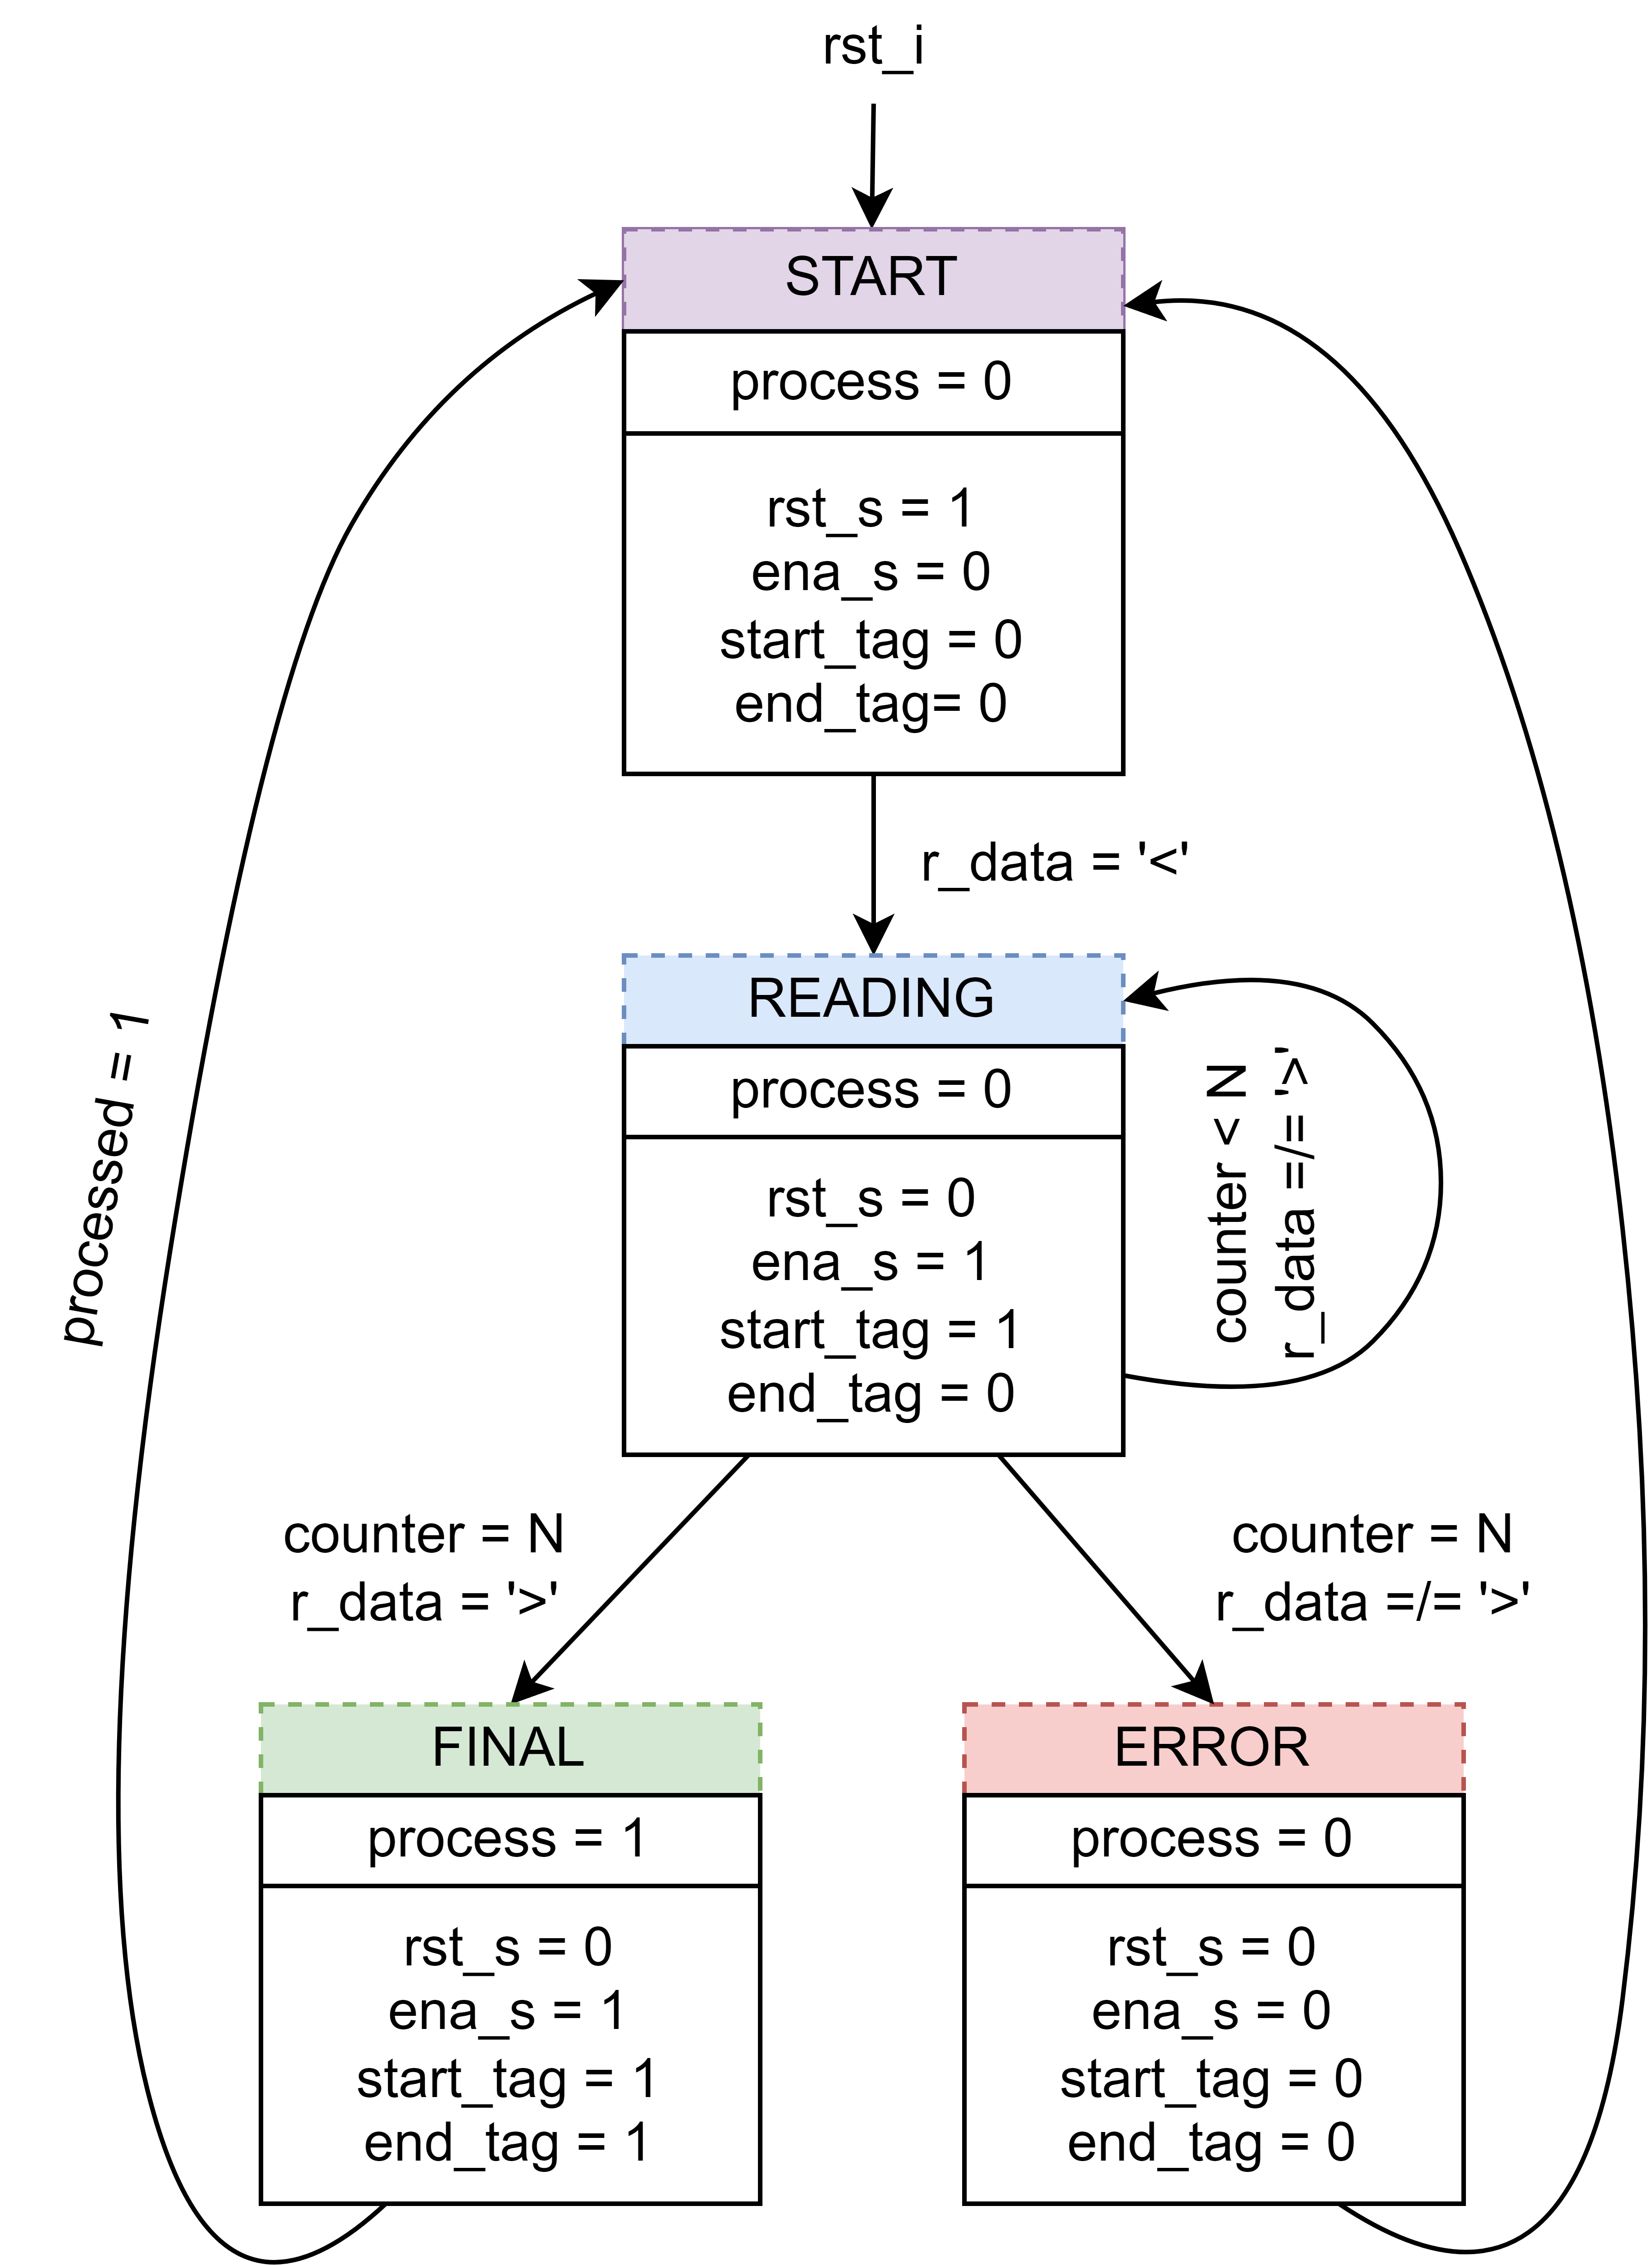
\includegraphics[width=0.8\textwidth]{Figuras/Detector_FSMD.png}
		\centering\caption{Diagrama de estados del módulo \textit{Detector}.}
		\label{fig:Detector_FSMD}
	\end{figure}
	
	El módulo \textit{Detector} inicia por detecto en el estado \textit{start}, aguardando por el caracter de inicio de trama '$<$'. Al recibir el caracter de inicio de trama, el módulo transiciona al estado \textit{reading}. En el estado \textit{reading} se recibirán solamente los caracteres ASCII '0' y '1'. Si al terminar de recibir N caracteres, el próximo caracter no es el de fin de trama '$>$' entonces se transiciona al estado \textit{error}, se reinician las variables auxiliares, la trama se descarta y se vuelve al estado \textit{start}.
	
	Si el próximo caracter luego de leer N valores ASCII '0' y '1' es el caracter de fin de trama '$>$', entonces el módulo transiciona al estado \textit{final}, donde se da por válida la trama y se habilita su envío al módulo \textit{decoder}, para volver al estado \textit{start} a la espera de un nuevl caracter de inicio de trama, reiniciando todas las variables auxiliares.
	
	Internamente se tienen diversas variables auxiliares para controlar si se han recibido los delimitadores y si la cantidad recibida es correcta. Eso cobra gran importancia al realizar los ensayos, porque se puede diferenciar rápidamente la fuente de posibles errores.
	\subsection{Módulo Decoder}
	\label{sec:decoder}
	
	El módulo \textit{Decoder} (ver Figura \ref{fig:GeneralSystem}) es el encargado de demultiplexar la trama \textit{packet}[N] ya validada por el módulo \textit{Detector}. El módulo \textit{Decoder} recibe el vector de elementos booleanos \textit{packet}[N] y la señal \textit{process} que indica cuando puede iniciar el proceso de demultiplexación. La salida serán todos los vectores de estado de los elementos ferroviarios. El diagrama de bloques de la máquinas de estado finitas con camino de datos se muestra en la Figura \ref{fig:Decoder_module}. En este caso particular, no se cuenta con una máquina de estados, ya que la demultiplexación se realiza directamente.
	
	\begin{figure}[H]
		\centering
		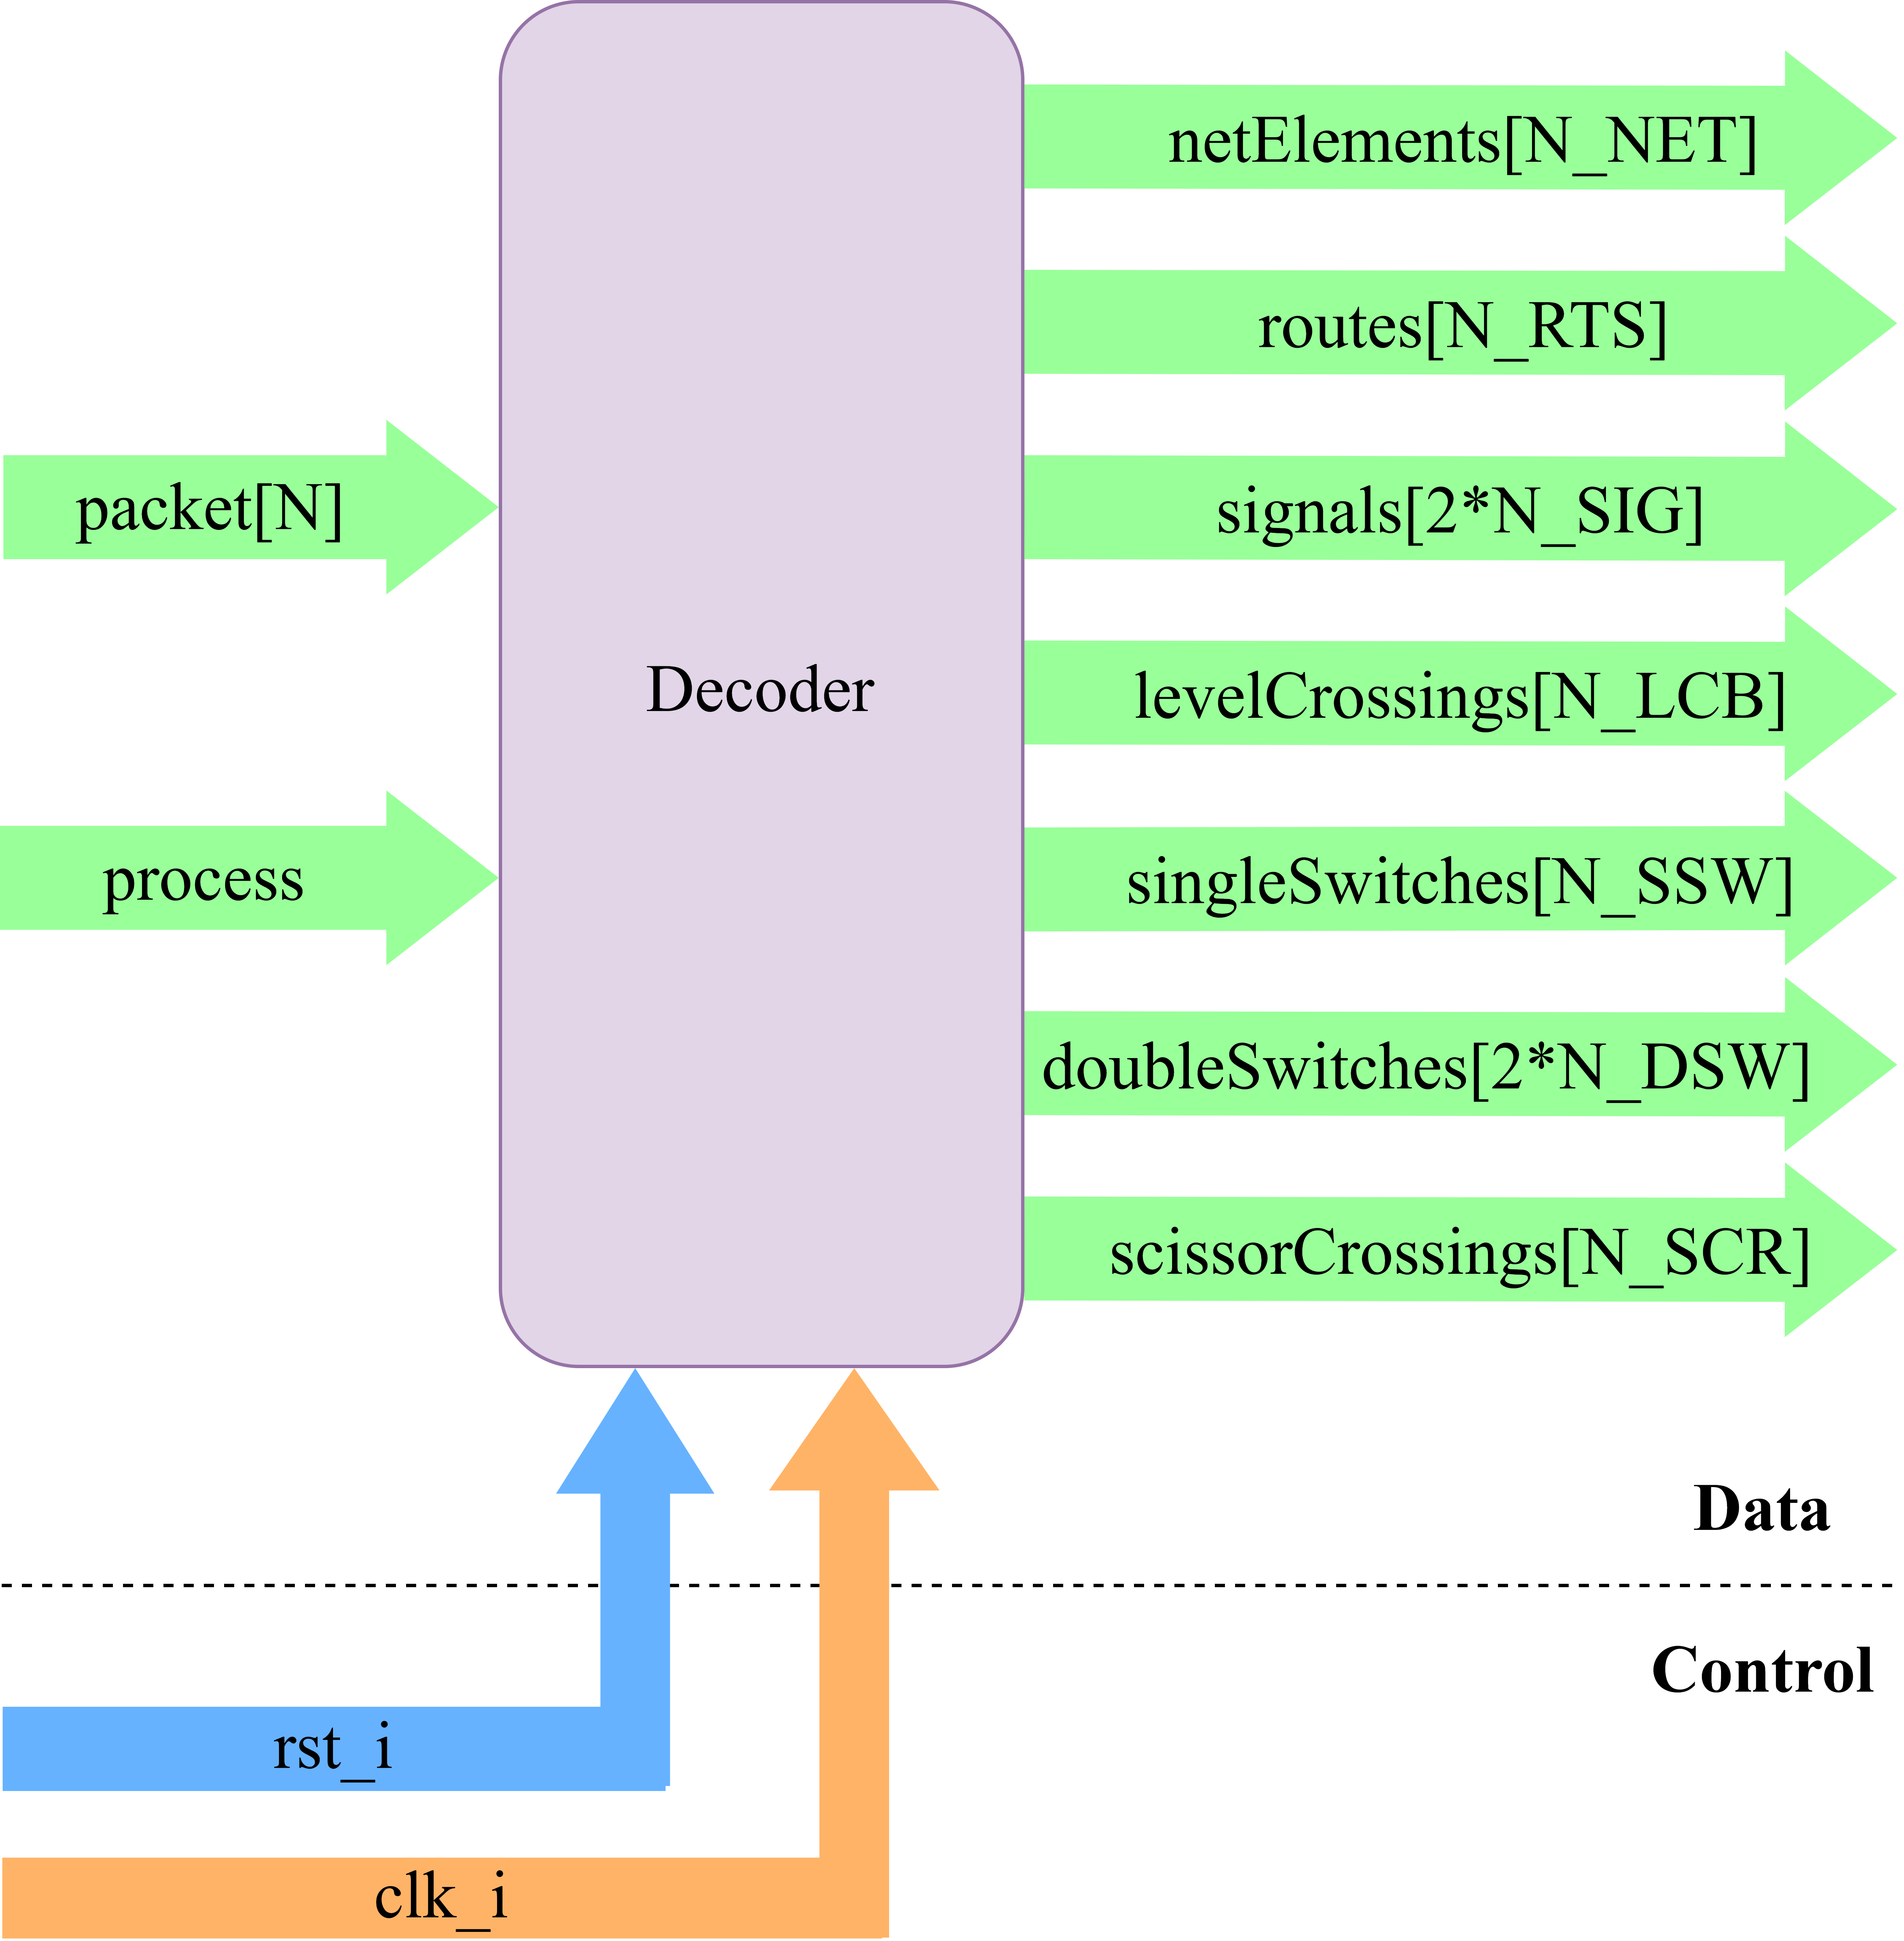
\includegraphics[width=1\textwidth]{Figuras/Decoder_module.png}
		\centering\caption{FSMD del módulo \textit{Decoder}.}
		\label{fig:Decoder_module}
	\end{figure}
	
	 La porción de \textit{packet}[N] correspondiente a cada vector será en función de la cantidad de elementos de cada tipo presentes en la locación. Esto ya fue calculado previamente por el ACG y explicado en la Sección \ref{sec:UART} al definir el formato de la trama. Si la cantidad de un cierto elemento ferroviario es mayor que uno, el ACG implementará el estado de ese elemento con un vector hexadecimal del tamaño adecuado. Si solo existe un elemento ferroviario de ese tipo, el ACG implementará un escalar hexadecimal. Si no existiese ningún elemento ferroviario en la locación, el ACG no implementará ninguna de las funcionalidades relativas a dicho elemento, optimizando el uso de recursos en la FPGA.
	\subsection{Módulo Encoder}
	\label{sec:encoder}
	
	El módulo \textit{Encoder} (ver Figura \ref{fig:GeneralSystem}) es el encargado de multiplexar los vectores de estado provenientes del módulo \textit{Network} y reconstruir una nueva trama, esta vez sin los valores de ocupación de vías por ser de sólo lectura. Esta nueva trama será \textit{packet}[N], junto con la señal \textit{processed} para indicar al módulo \textit{Printer} que la trama está completa y lista para ser transmitida. El diagrama de bloques de las máquinas de estado finitas con camino de datos se muestra en la Figura \ref{fig:Encoder_module}.
	
	\begin{figure}[H]
		\centering
		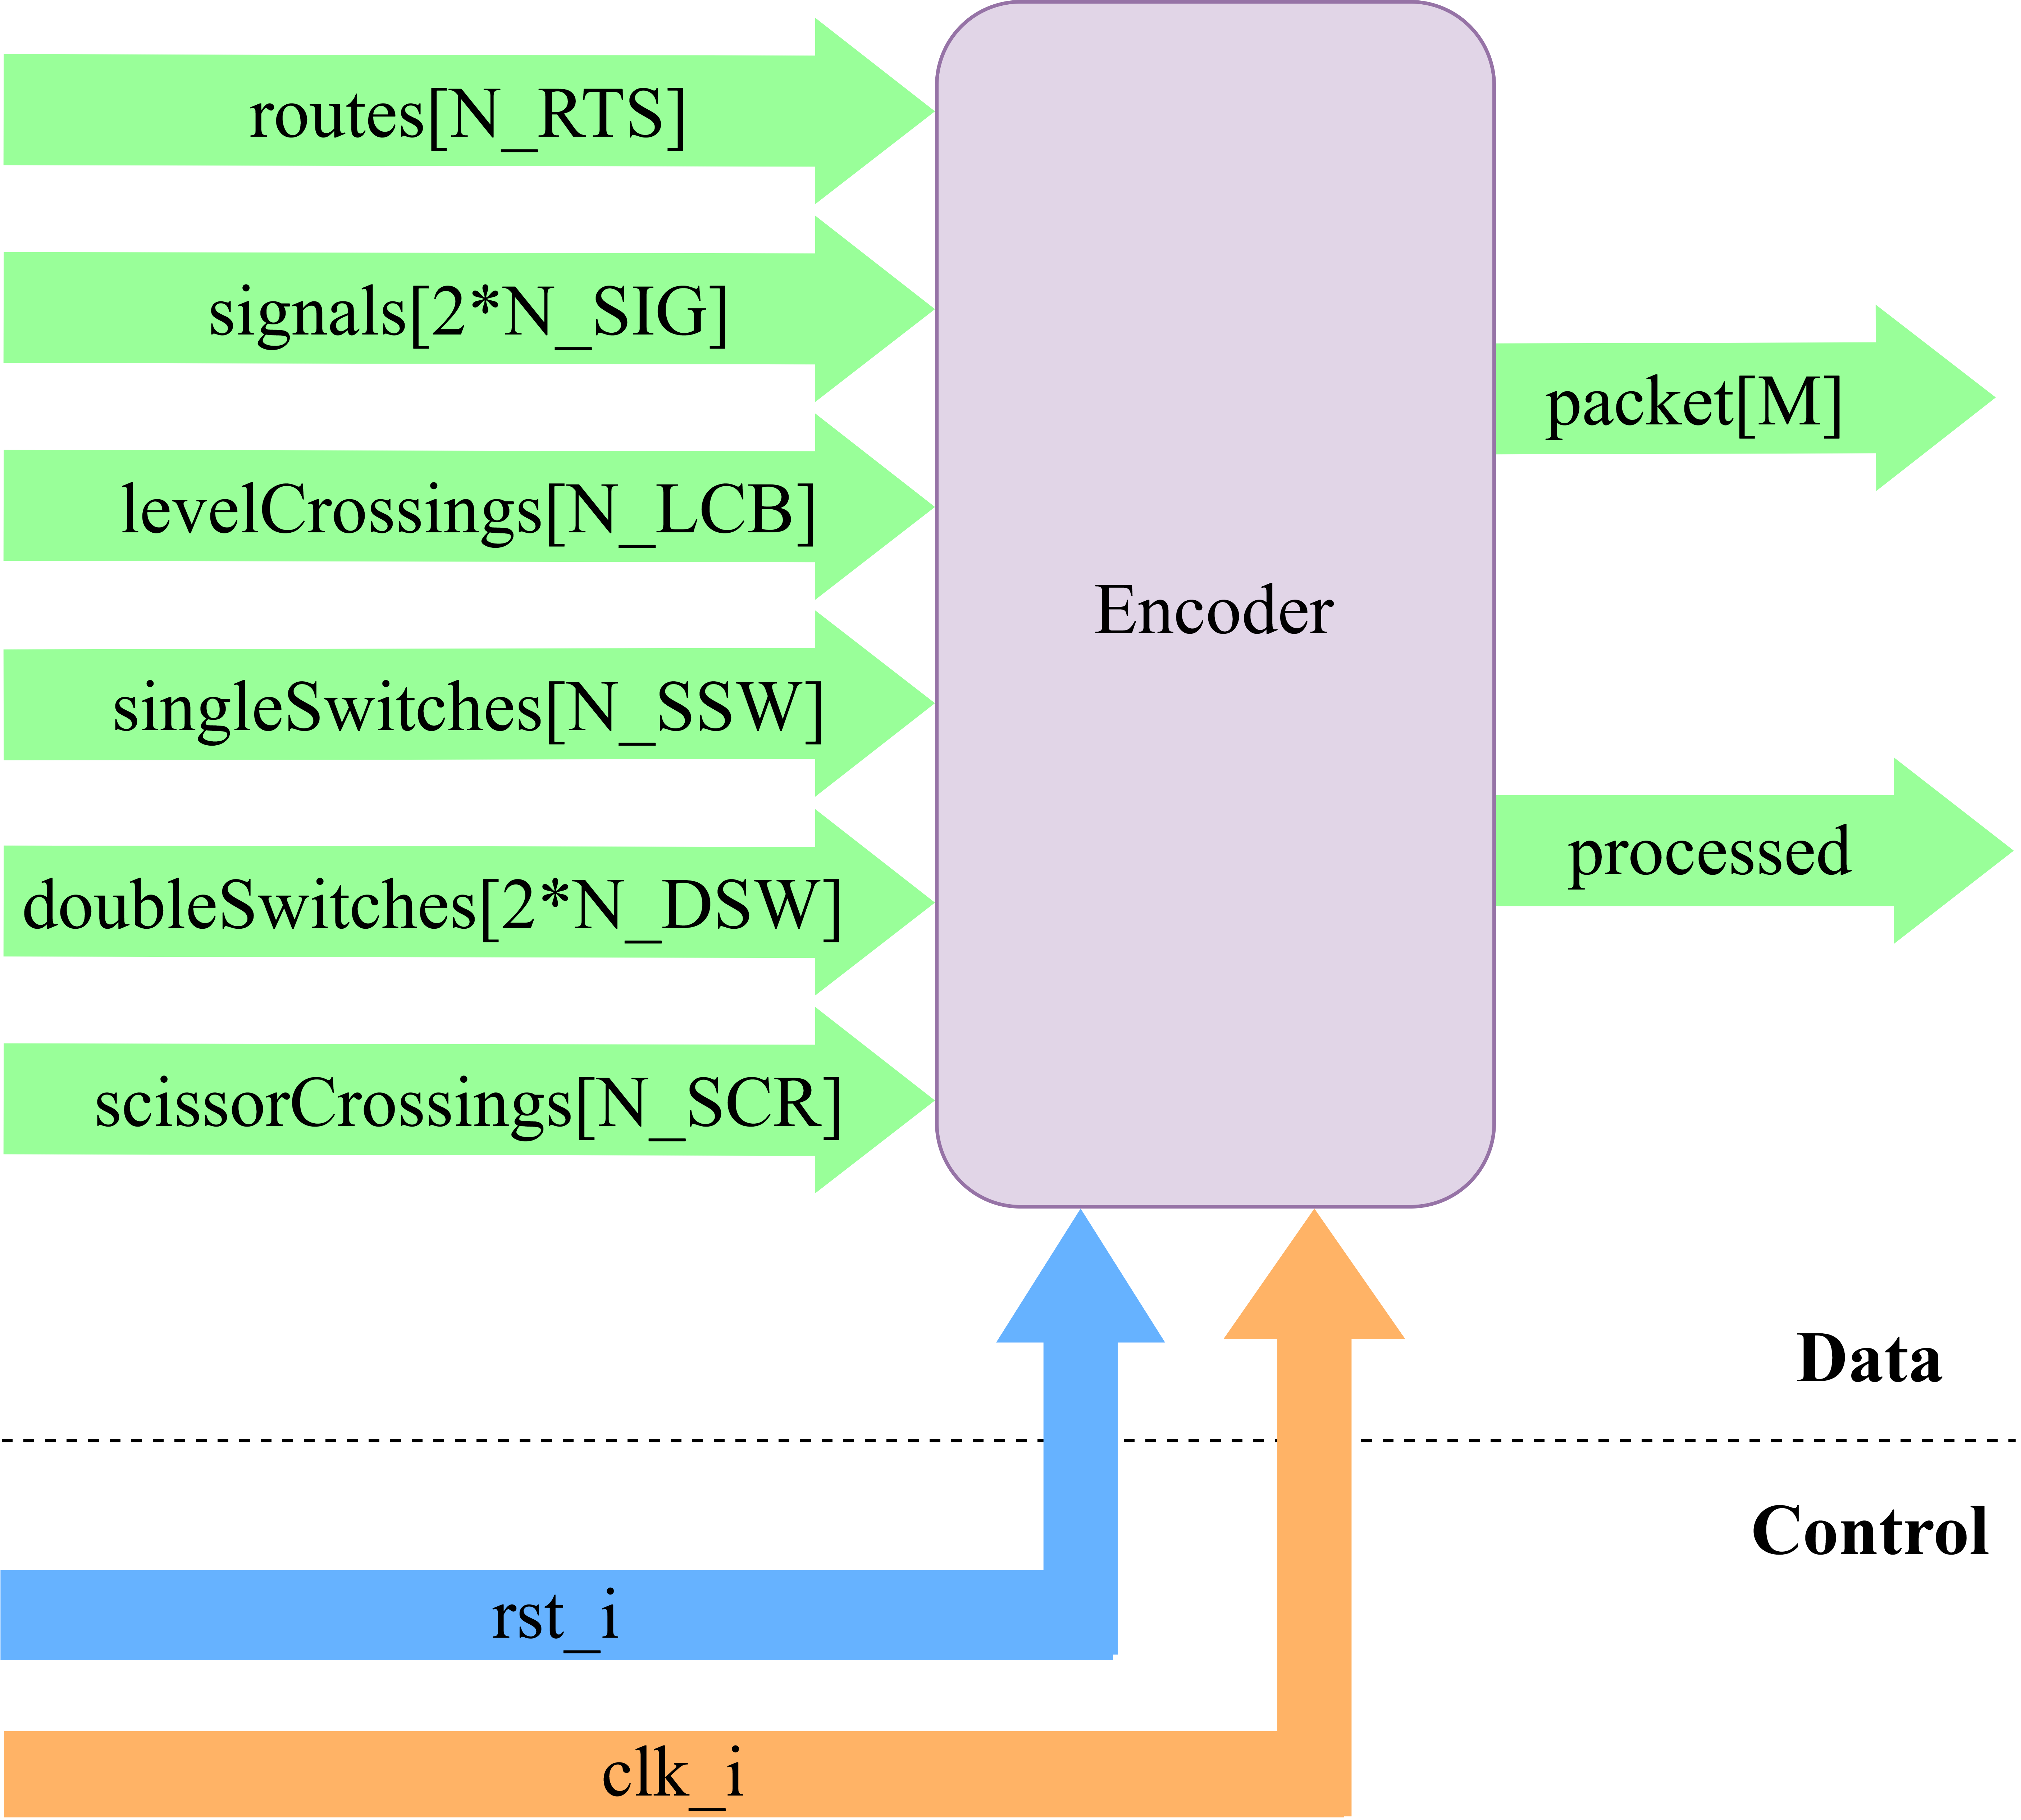
\includegraphics[width=1\textwidth]{Figuras/Encoder_module.png}
		\centering\caption{FSMD del módulo \textit{Encoder}.}
		\label{fig:Encoder_module}
	\end{figure}
	
	Al igual que la demultiplexación que realiza el módulo \textit{Decoder}, la multiplexación se basa en la cantidad de elementos ferroviarios de cada tipo, calculdos por el ACG al definir la trama tal cual fue explicado en la Sección \ref{sec:UART}. Los elementos inexistentes en la locación no serán tenidos en cuenta para formar la nueva trama, reduciendo el tamaño de la misma al mínimo.
	\subsection{Módulo Printer}
	\label{sec:printer}
	
	El módulo Printer (ver Figura \ref{fig:GeneralSystem}) realiza la conversión de cada elemento de un vector de M elementos hexadecimales (\textit{packet}[M], M elementos de 4 bits) en caracteres hexadecimales (1 byte). Cada elemento del vector es analizado en cada ciclo de reloj (clk\_i) y demultiplexado, de manera tal de convertir un elemento por vez, para luego enviar el byte correspondiente al módulo UART para su posterior transmisión al exterior. El diagrama de bloques de la máquina de estados finitos con camino de datos se muestra en la Figura \ref{fig:Printer_module}.
	
	\begin{figure}[H]
		\centering
		\includegraphics[width=1\textwidth]{Figuras/Printer_module.png}
		\centering\caption{FSMD del módulo \textit{Printer}.}
		\label{fig:Printer_module}
	\end{figure}
	
	En cada ciclo de reloj el módulo \textit{Printer} demultiplexa el vector \textit{packet}[M] para obtener un elemento lógico que procesar, según el valor del contador vigente, que se incrementa en cada ciclo, hasta un máximo de M-1. Si el elemento \textit{packet}[i] es un valor hexadecimal, se enviará un byte equivalente en ASCII. Por ejemplo, se enviará un byte equivalente al 'A' ASCII si el elemento \textit{packet}[i] es una 'A' hexadecimal.
	
	Cada dos ciclos de reloj el módulo \textit{Printer} genera un pulso para habilitar el envío del último byte generado. Junto con el caracter se envía la señal \textit{wr\_uart} para indicarle a la UART que ese dato debe ser guardado en la FIFO de salida y la señal \textit{processed} para indicarle al módulo \textit{Detector} que se pueden procesar nuevas tramas. El ciclo de procesamiento de la trama a transmitir se describe el diagrama de estados de la Figura \ref{fig:Printer_FSMD}.
	
	\begin{figure}[H]
		\centering
		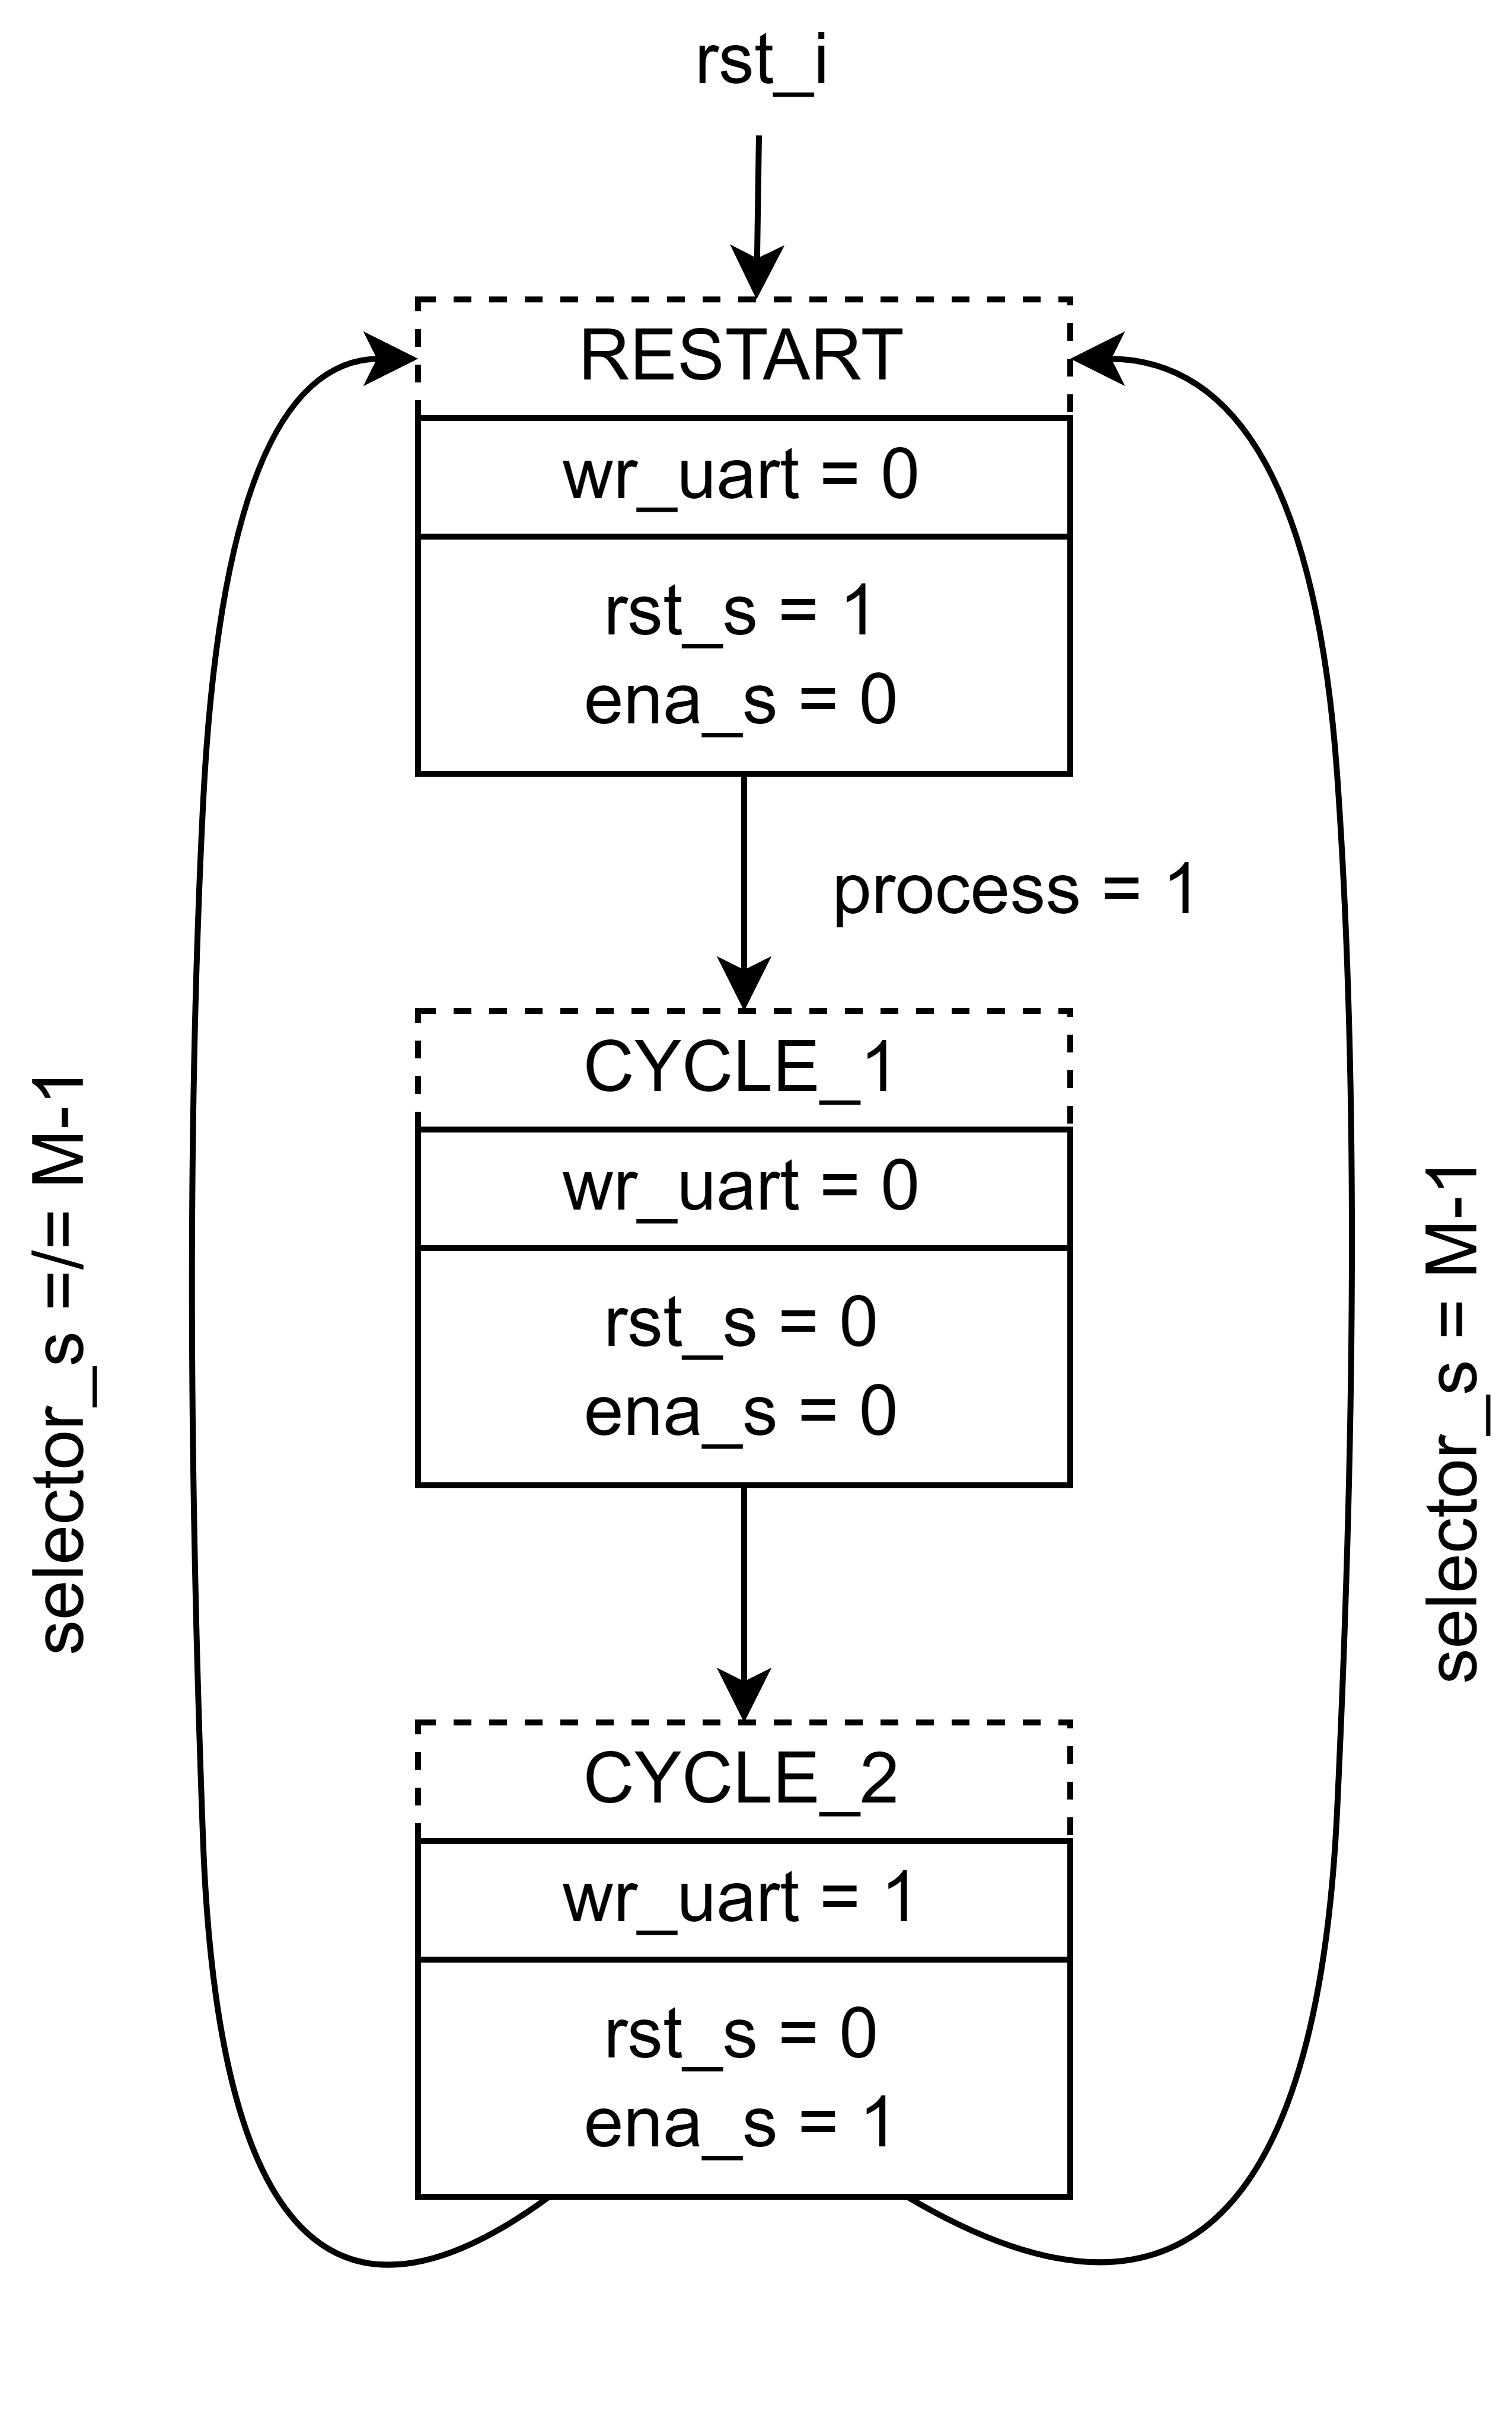
\includegraphics[width=0.8\textwidth]{Figuras/Printer_FSMD.png}
		\centering\caption{Diagrama de estados del módulo \textit{Printer}.}
		\label{fig:Printer_FSMD}
	\end{figure}
	
	El módulo \textit{Printer} inicia por detecto en el estado \textit{restart}, a la espera de recibir la señal \textit{process} del módulo \textit{Encoder}. Se tienen dos estados (\textit{cycle\_1} y \textit{cycle\_2}) para generar el pulso de reloj necesario para mantener sincronizadas las tramas. Cuando el contador haya recorrido los M elementos de \textit{packet}[M], el módulo vuelve al estado \textit{restart}, para esperar una nueva señal \textit{process} para volver a procesar una nueva trama de datos.
	
	Si la trama recibida es incorrecta, o si ya fue impresa, entonces la señal \textit{process} será '0' y el modulo \textit{Printer} dejará de enviar datos a la UART. Si la señal \textit{process} mantiene un estado lógico positivo, el proceso de impresión continuará hasta que la UART indique que no pueda recibir mas datos o que alguna etapa previa informe de algún error en el proceso.
	\subsection{Módulo Selector}
	\label{sec:selector}
	
	Se añadió el módulo \textit{Selector} (ver Figura \ref{fig:GeneralSystem}) para poder facilitar el testeo de la comunicación serial al permitir anular la totalidad del sistema de enclavamiento. De esta manera, es posible validar la lectura, detección y escritura de tramas en bucle en forma independiente al sistema de enclavamiento. Esta funcionalidad es habilitada cambiando la posición de un switch físico de la FPGA y se desactiva invirtiendo su posición. El diagrama de bloques de la máquina de estados finitos con camino de datos diseñado para lograr este objectivo se muestra en la Figura \ref{fig:Selector_module}.
	
	\begin{figure}[H]
		\centering
		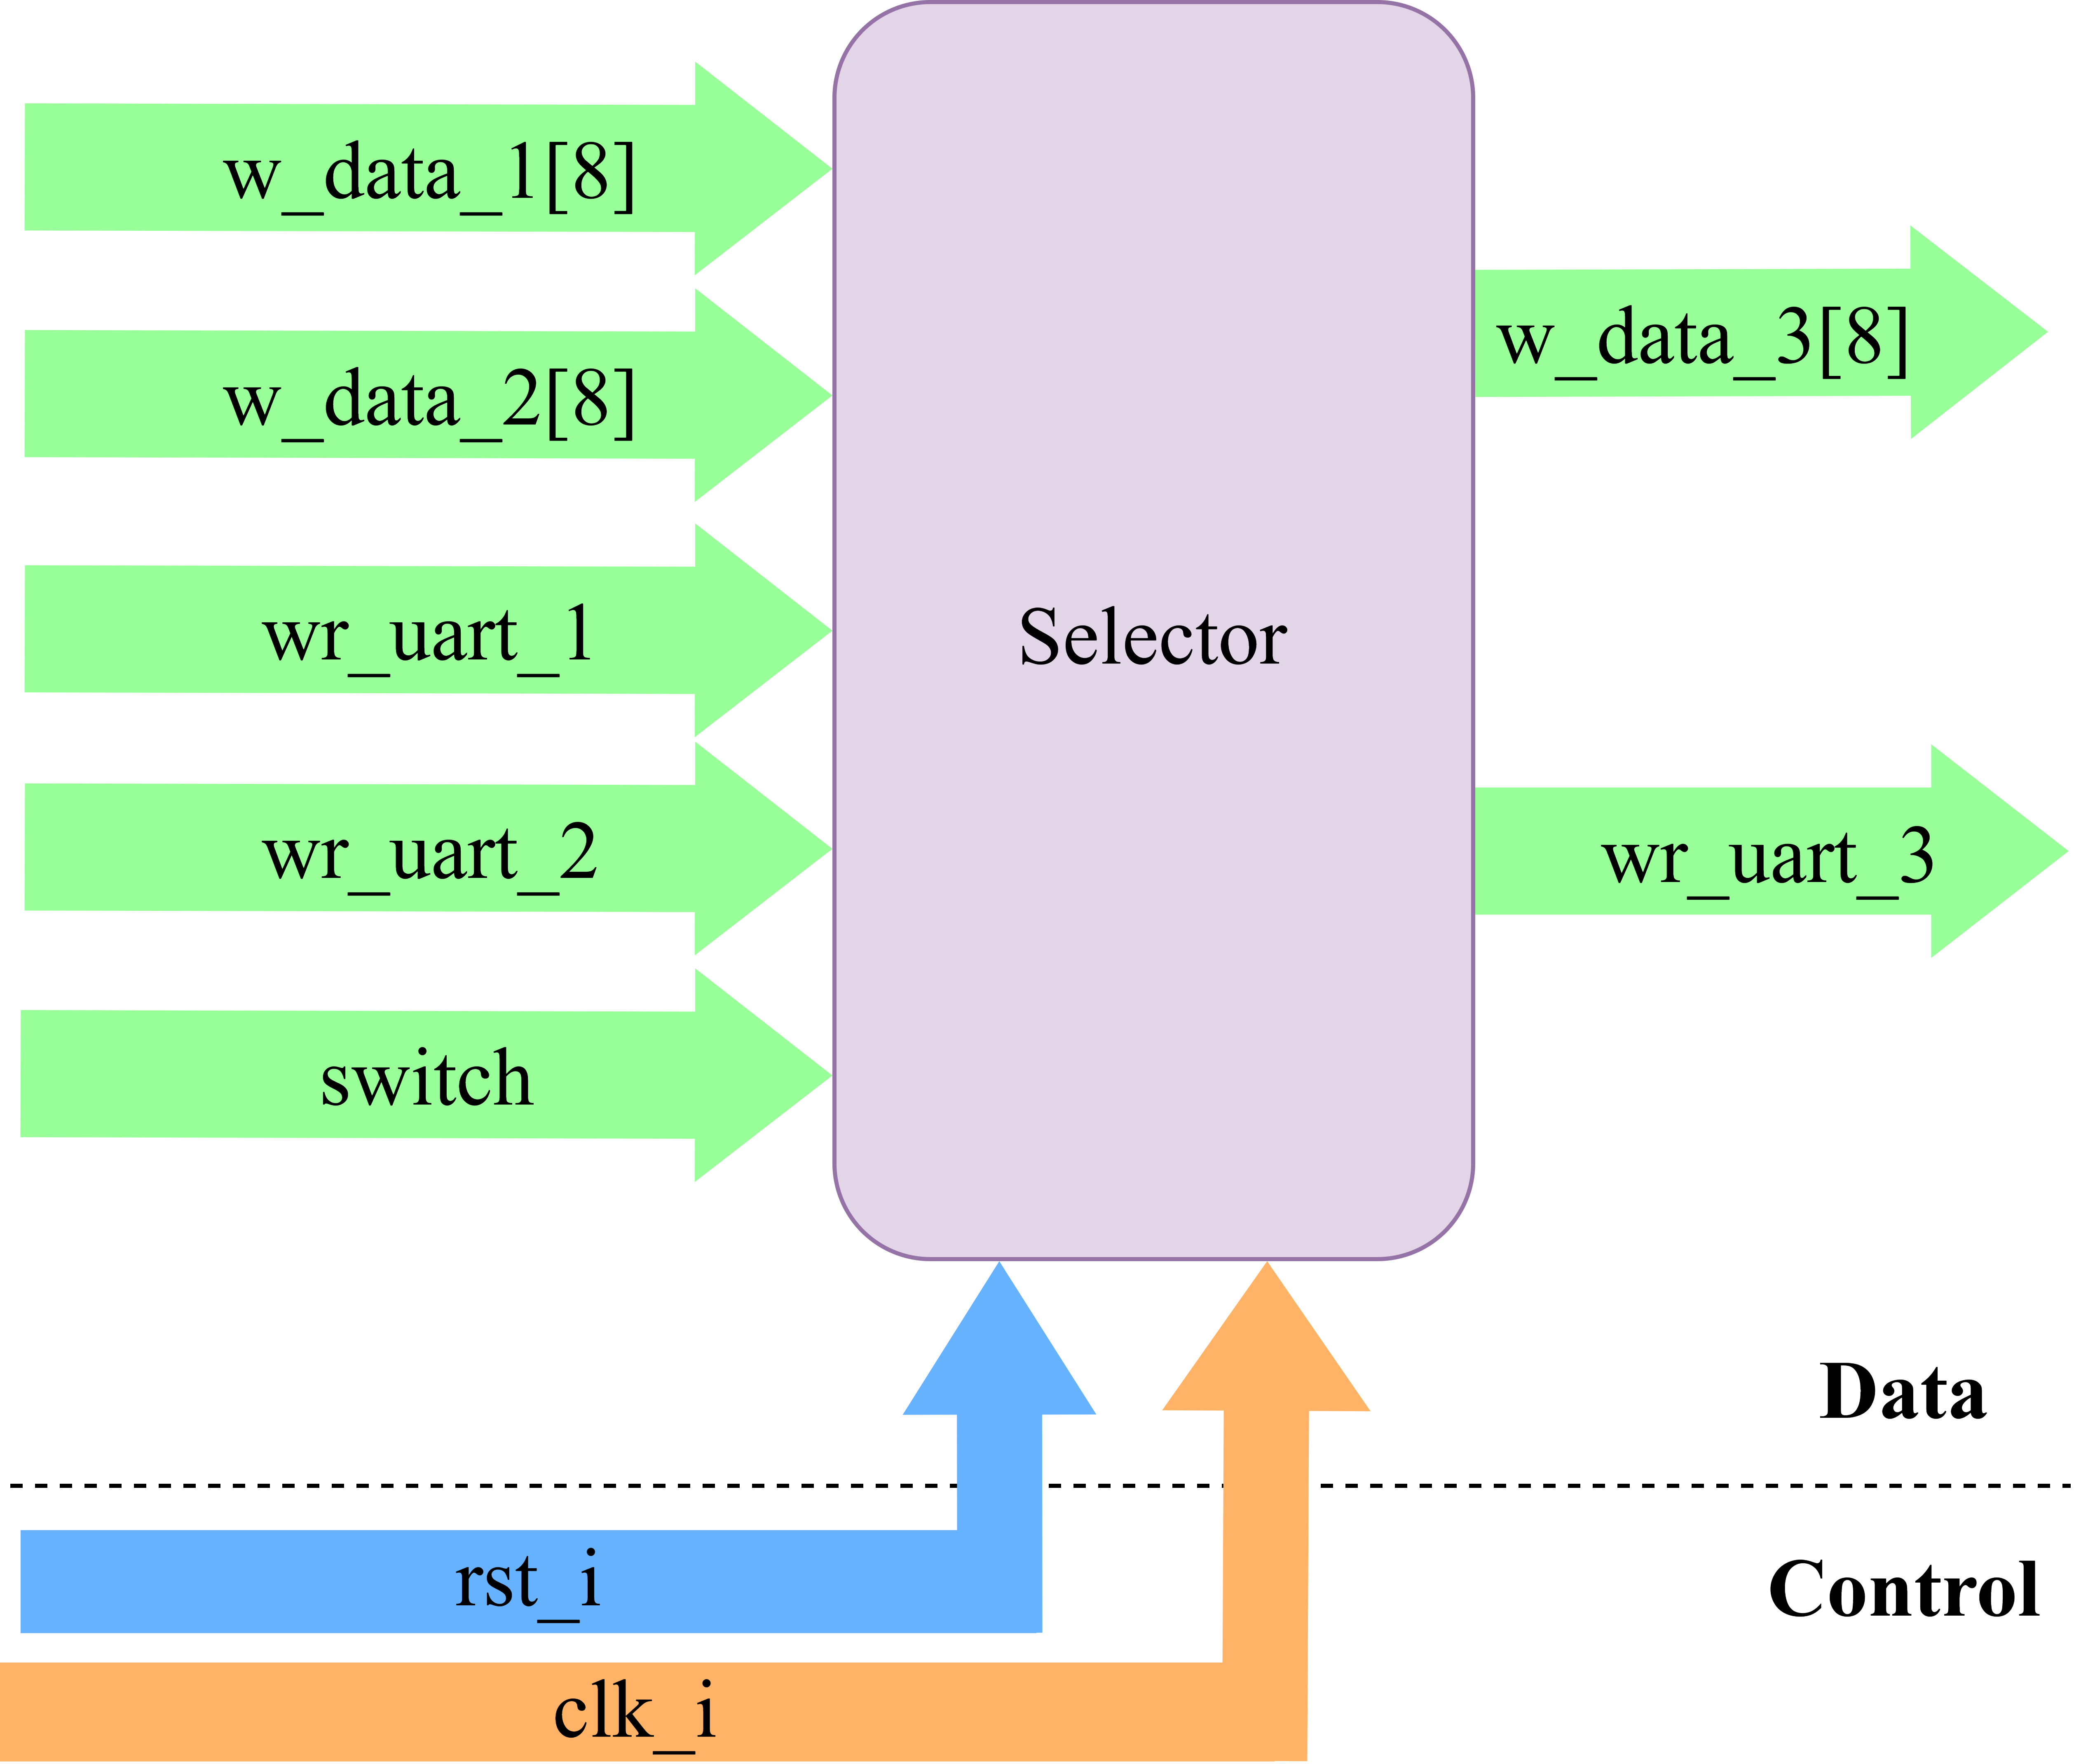
\includegraphics[width=0.55\textwidth]{Figuras/Selector_module.png}
		\centering\caption{FSMD del módulo \textit{Selector}.}
		\label{fig:Selector_module}
	\end{figure}
	\subsection{Modulo Network}

El módulo \textit{Network} es el encargado de instanciar todos los elementos ferroviarios presentes en la red de grafos generada por el RNA e interconectarlos como ésta indica. Es el módulo que mas recursos de la FPGA utiliza y donde más se hace énfasis en el uso óptimo de los recursos. Se prioriza la máxima descentralización posible de los módulos instanciados internamente, de forma tal que cada uno de ellos solo dependa de la mínima cantidad necesaria de módulos, evitando conexiones innecesarias. El diagrama de bloques de las máquinas de estado finitas con camino de datos diseñado para lograr este objetivo se muestra en la Figura \ref{fig:Network_module}.

\begin{figure}[H]
	\centering
	\includegraphics[width=1\textwidth]{Figuras/Network_module.png}
	\centering\caption{FSMD del módulo \textit{Network}.}
	\label{fig:Network_module}
\end{figure}

Los módulos de \textit{NetElements}, \textit{Routes} y \textit{Signals} son obligatorios ya que se encuentran presentes en la mínima red ferroviaria aceptada por el RNA. En cambio, los módulos de \textit{SingleSwitches}, \textit{DoubleSwitches}, \textit{ScissorCrossings} y \textit{LevelCrossings} son opcionales y dependen de que existan en la locación. Es decir, si un elemento ferroviario no existe, no solamente no serán instanciado por el ACG, sino que tampoco se generarán archivos que definan sus módulos, señales auxiliares que los interconecten a otros módulos ni tampoco entradas o salidas en otros módulos, destinados a este elemento. De esta manera, se reduce la complejidad del sistema enormemente al implementar solamente los puertos, señales, módulos y conexiones que serán utilizados por el sistema de enclavamiento.

Para garantizar la descentralización de la red, a todos los elementos ferroviarios con entidad física, es decir, todos los mencionados menos las rutas que son entidades abstractas, se les implementa la propiedad de enclavamiento. El enclavamiento de un elemento puede presentar tres estados, tal como se describe en la Tabla \ref{Tab:interlock_states}.

	\begin{table}[!h]
	{
		\caption{Estados de enclavamiento de cada elemento ferroviario.}
		\label{Tab:interlock_states}
		\centering
		\resizebox{1\textwidth}{!}{
		\begin{tabular}{ p{5cm} p{4cm} p{4cm} }
			\hline	
			Liberado & Reservado & Enclavado \\	
			\hline
			Solicitado por cualquier ruta u opera de forma automática.& 
			Operado solamente por la ruta que lo reservó.&
			Depende de sí mismo y de la ruta que lo enclavó.\\
			\hline
		\end{tabular}
		}
	}
	\end{table}

Todo elemento se encuentra por defecto en el estado liberado y puede ser solicitado por cualquier ruta. Tan pronto una ruta envía el comando de reserva al elemento, pasa a estar en estado reservado y ninguna otra ruta podrá hacer uso de este elemento. Finalmente, si la ruta ha podido reservar todos los elementos necesarios para cumplir las condiciones para ser habilitada, enviará la señal de enclavamiento a todos los elementos involucrados, evitando que puedan ser comandados por otras rutas. Esto incluye tanto a la ocupación de vías (\textit{NetElements}) como a las señales (\textit{Signals}), pasando por todos los cambios de vías (\textit{SingleSwitches}, \textit{DoubleSwitches} y \textit{ScissorCrossings}) y barreras de pasos a nivel (\textit{LevelCrossings}). De esta manera el ACG se asegura que cada elemento sea controlado por una única ruta por vez o de forma automática si ninguna ruta demanda su uso.

Para generalizar y modelizar el comportamiento dinámico del enclavamiento los elementos ferroviarios recurrimos a las redes de Petri \cite{Paper_64,Paper_65,Paper_88,Paper_94,Paper_95,Paper_123,Paper_196}. Una red de Petri es la representación gráfica de un modelo matemático de autómatas concurrente. Las mismas están formadas por lugares (el estado), las transiciones que concentran las condiciones para pasar de un lugar a otro y los arcos que conectan lugares y transiciones. Las redes de Petri puede poseer uno o mas tokens que representan en que estado se encuentra el sistema. Algunas redes de Petri admiten mas de un token por red, o incluso mas de un token por lugar. En el caso del sistema de enclavamiento se definieron solamente redes de Petri con un único token por red, siendo que el sistema solo puede adoptar un estado en cada momento. En la Figura \ref{fig:Interlocking_petri} se visualiza el modelo matemático del enclavamiento de un elemento ferroviario genérico.

\begin{figure}[H]
	\centering
	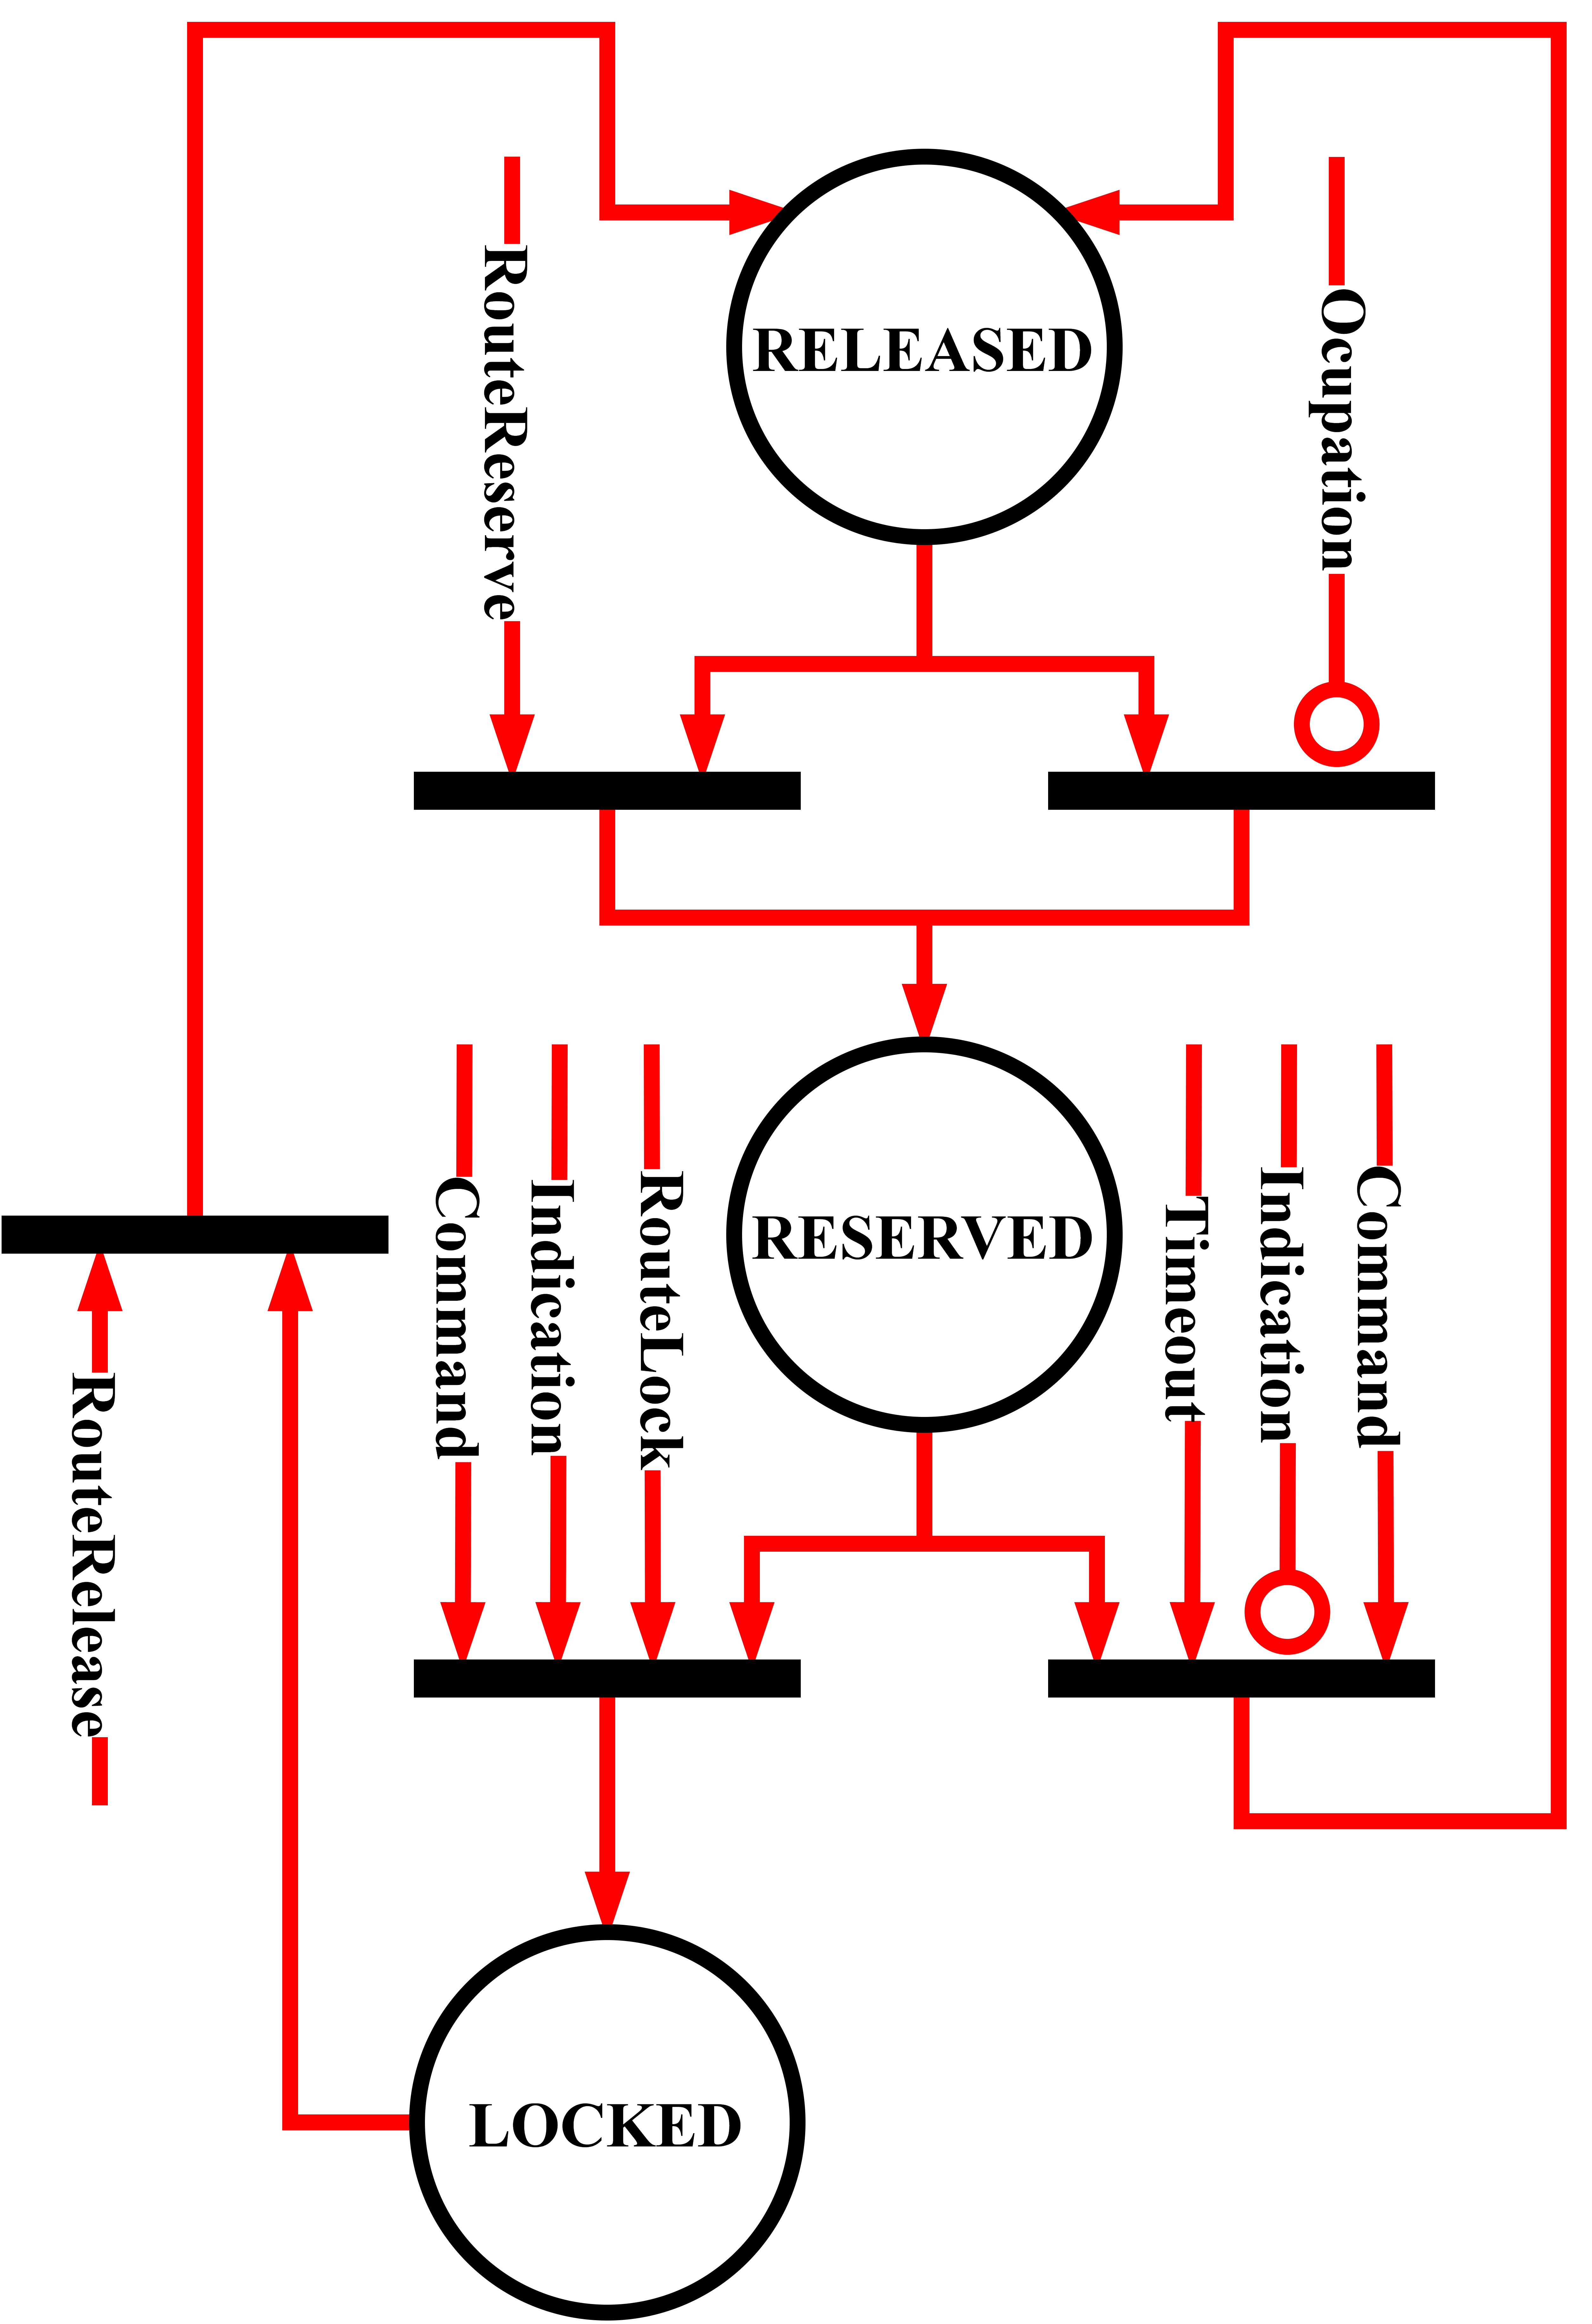
\includegraphics[width=0.7\textwidth]{Figuras/INT_petri}
	\centering\caption{Red de Petri del modelo dinámico de enclavamiento de elementos ferroviarios genéricos.}
	\label{fig:Interlocking_petri}
\end{figure}

La transición de un elemento ferroviario del estado liberado a reservado no solo puede darse por el pedido expreso de una ruta que lo solicite, sino también de facto al ocuparse los netElements cercanos al elemento, lo cual inicia lo que se denomina 'bloqueo por ocupación' (ver Sección XXX). Esto protege al sistema al impedir que otras rutas soliciten un cambio de estado de un elemento que esta siendo usado por una formación que no ha solicitado ningún permiso, reduciendo el riesgo de accidentes por descarrillamiento o colisión. La red de Petri también deja explícito la inclusión de un timeout para las reservas, con un valor por defecto de 7 segundos, configurable por el usuario. De no cumplirse que el comando y la indicación coincidan dentro del tiempo estipulado, el elemento es liberado, siempre que no se encuentren formaciones cercanas. Las transición de reserva a enclavamiento requiere que tanto el comando como la indicación coincidan y que la ruta solicite el enclavamiento al haber confirmado que todas las condiciones de ruta se han cumplido y es inminente su habilitación. El elemento ferroviario deja de estar enclavado cuando la ruta lo solicita expresamente, momento en el cuál pasa a estar liberado para que otras rutas puedan usarlo.

A diferencia de los módulos explicados en secciones anteriores, donde cada módulo era instanciado una vez, los módulos que modelan elementos ferroviarios, con entidad física o abstracta, son instanciados tantas veces como unidades de éstos existan. Es por eso que, en las siguientes secciones, hablaremos de módulos genéricos a la hora de describir cada módulo. Estos módulos genéricos presentarán todas las entradas, salidas y funcionalidades que pueden tener, de ser requeridas. 

Es trabajo del ACG determinar cuales de ellas deben ser implementadas y cuales no. Por ejemplo, si una ruta A requiere que una barrera X se encuentre baja, pero no tiene requerimientos respecto a las posiciones de los cambios porque la ruta A no los utiliza, entonces el ACG instanciará el módulo de la ruta A considerando en las entradas y salidas los estados de la barrera X y los comandos para operarla, intercontando el módulo de ruta A con el módulo de la barrera ferroviaria X. En cambio, el ACG no implementará ningún puerto destinado a los cambios de vías ni lo considerará en las funcionalidades del módulo de ruta A. De igual manera, el ACG conectará los estados de ocupación de vías correspondientes solamente a los módulos de los elementos ferroviarios que los necesitan y no la totalidad del vector de datos.

\subsection{Módulo genérico de las barreras ferroviarias}

El módulo \textit{LevelCrossing} es el encargado de implementar el funcionamiento de las barreras ferroviarias en los pasos a nivel. El ACG utiliza la información otorgada por el RNA para determinar cuál es el netElement donde se sitúa el paso a nivel y cuales son los netElements mas próximos, para que puedan reportar su estado al módulo \textit{LevelCrossing}. Además, el ACG implementará todas las conexiones para cada una de las rutas en las cuales el paso a nivel sea condición necesaria para su habilitación. El diagrama de bloques de las máquinas de estado finitas con camino de datos diseñado para lograr este objetivo se muestra en la Figura \ref{fig:Network_module}.

\begin{figure}[H]
	\centering
	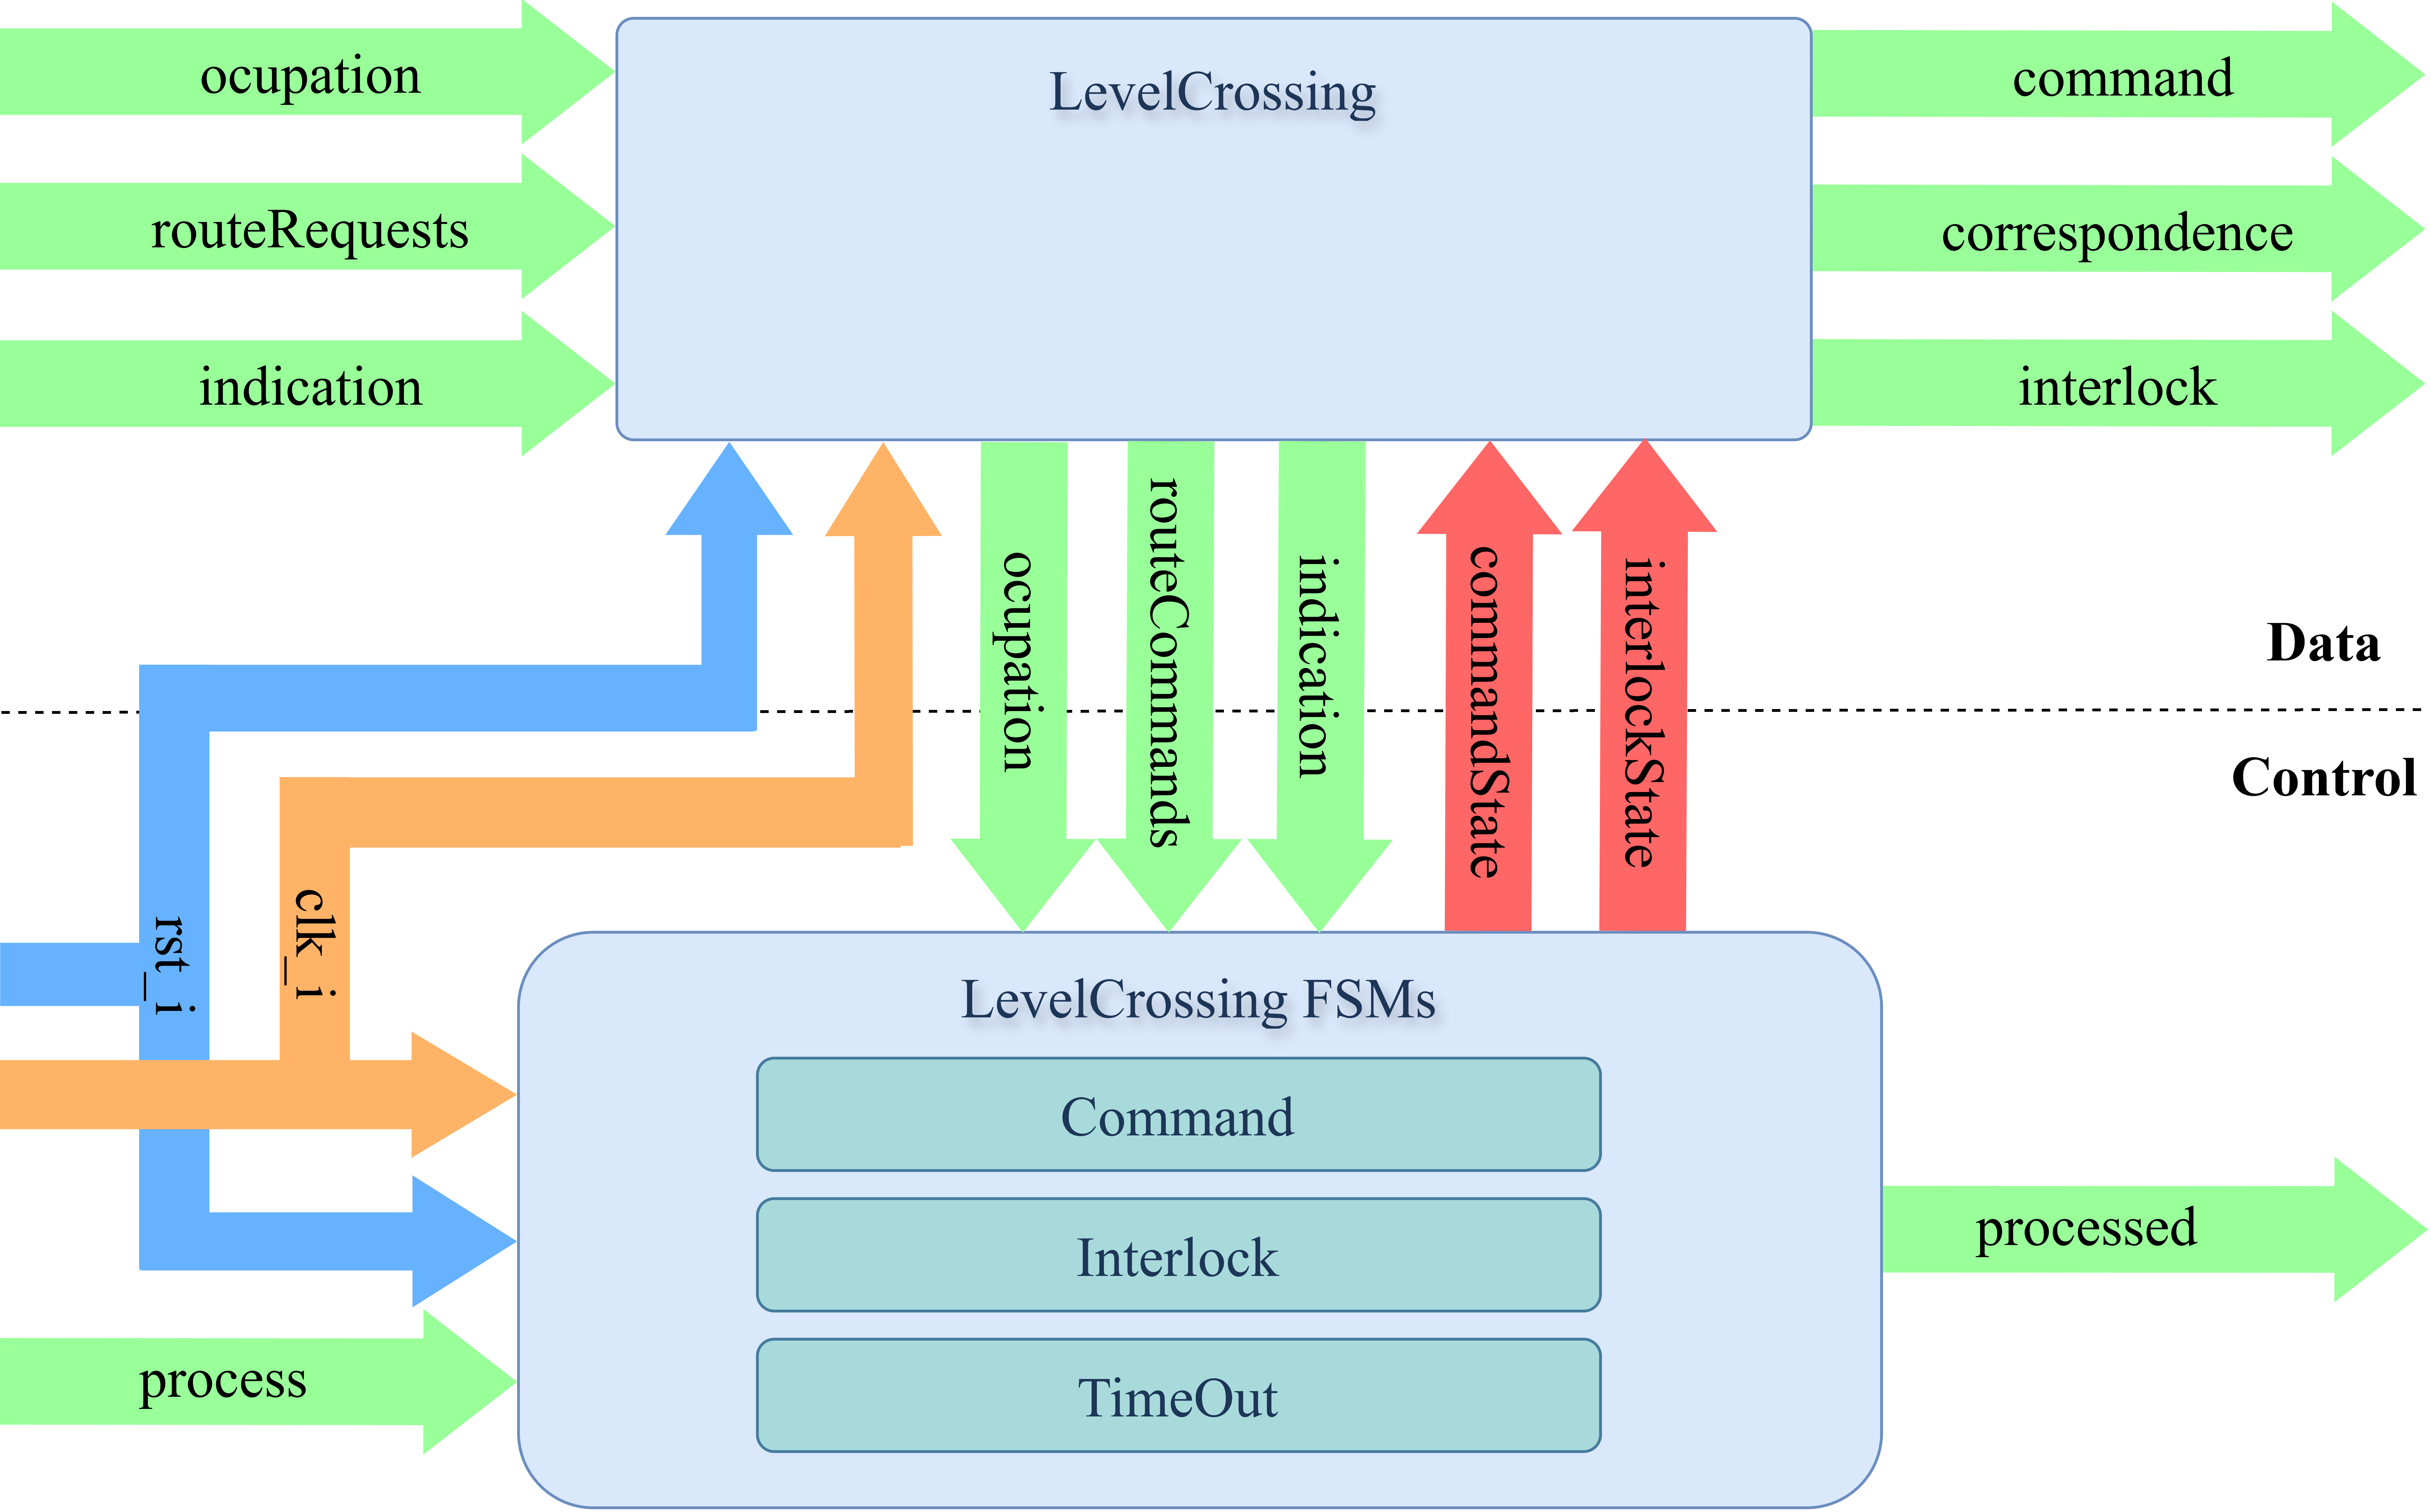
\includegraphics[width=1\textwidth]{Figuras/LCB_module}
	\centering\caption{FSMD del módulo genérico de \textit{LevelCrossing}.}
	\label{fig:LCB_module}
\end{figure}

Tal como se explicó en la Sección \ref{sec:switches}, las barreras ferroviarias también poseen comando, indicación y correspondencia. Comando para controlar la barrera, indicación para reportar su estado actual al módulo \textit{LevelCrossing} y correspondencia para declarar su estado final a la ruta que lo solicite. Además, el ACG implementará todas las conexiones necesarias a todas las rutas que tengan a la barrera en cuestión como condición necesaria de habilitación. Finalmente, el módulo \textit{LevelCrossing} tiene una salida que define su estado de enclavamiento frente a otras rutas que lo requieran.

El comportamiento de una barrera de paso a nivel genérico se define en la red de Petri de la Figura \ref{fig:LCB_Petri}. Una barrera se mantendrá en estado alto a menos que una ruta solicite que el brazo de barrera descienda o si los \textit{netElements} cercanos se encuentran ocupados. Durante la transición se espera la confirmación de que la barrera ha descendido mientras se mantiene la ocupación para terminar el movimiento en el estado bajo. Estado en el cual solo podrá salir si la ocupación termina y ninguna ruta solicita que la barrera se mantenga baja.

\begin{figure}[H]
	\centering
	\includegraphics[width=1\textwidth]{Figuras/LCB_petri}
	\centering\caption{Red de Petri del modelo dinámico de \textit{LevelCrossing}.}
	\label{fig:LCB_Petri}
\end{figure}

Durante el estado de transición la barrera tendrá 7 segundos para llegar al estado bajo. Al cumplirse el tiempo, si la indicación y el comando no coinciden y los textit{netElements} cercanos se encuentran libres, la barrera volverá al estado alto. Esto impide que el sistema habilite rutas cuando los actuadores de algún elemento se atascan o su indicación es diferente al comando que se ha enviado. La confirmación de la indicación otorga un grado de seguridad mayor al no asumir que un comando enviado implica automáticamente que al actuador se le impone dicho estado.
\subsection{Módulo genérico de los cambios de vías simples}
	\label{sec:ACG_ssw}
	
	El módulo \textit{SingleSwitches} (ver Figura \ref{fig:GeneralSystem}) es el encargado de implementar el funcionamiento de los cambios de vías simples en la red ferroviaria. El ACG utiliza la información otorgada por el RNA para determinar cuales son los \textit{netElements} conectados mediante el cambio de vías, los \textit{netElements} más próximos. Esta información se utiliza para implementar las entradas del módulo \textit{SingleSwitches} donde se reporta el estado de ocupación de los \textit{netElements} (\textit{ocupation}). Además, se implementan las conexiones de indicación, comando y correspondencia para poder leer, escribir y reportar el estado del cambio de vías, respectivamente. Finalmente, el ACG implementa las conexiones a todas las rutas que buscarán controlar el cambio de vías y todo los mecanismos para obedecer solo a una de ellas, de cumplirse las condiciones. El diagrama de bloques de las máquinas de estado finitas con camino de datos diseñado para lograr este objetivo se muestra en la Figura \ref{fig:SSW_module}.
	
	\begin{figure}[H]
		\centering
		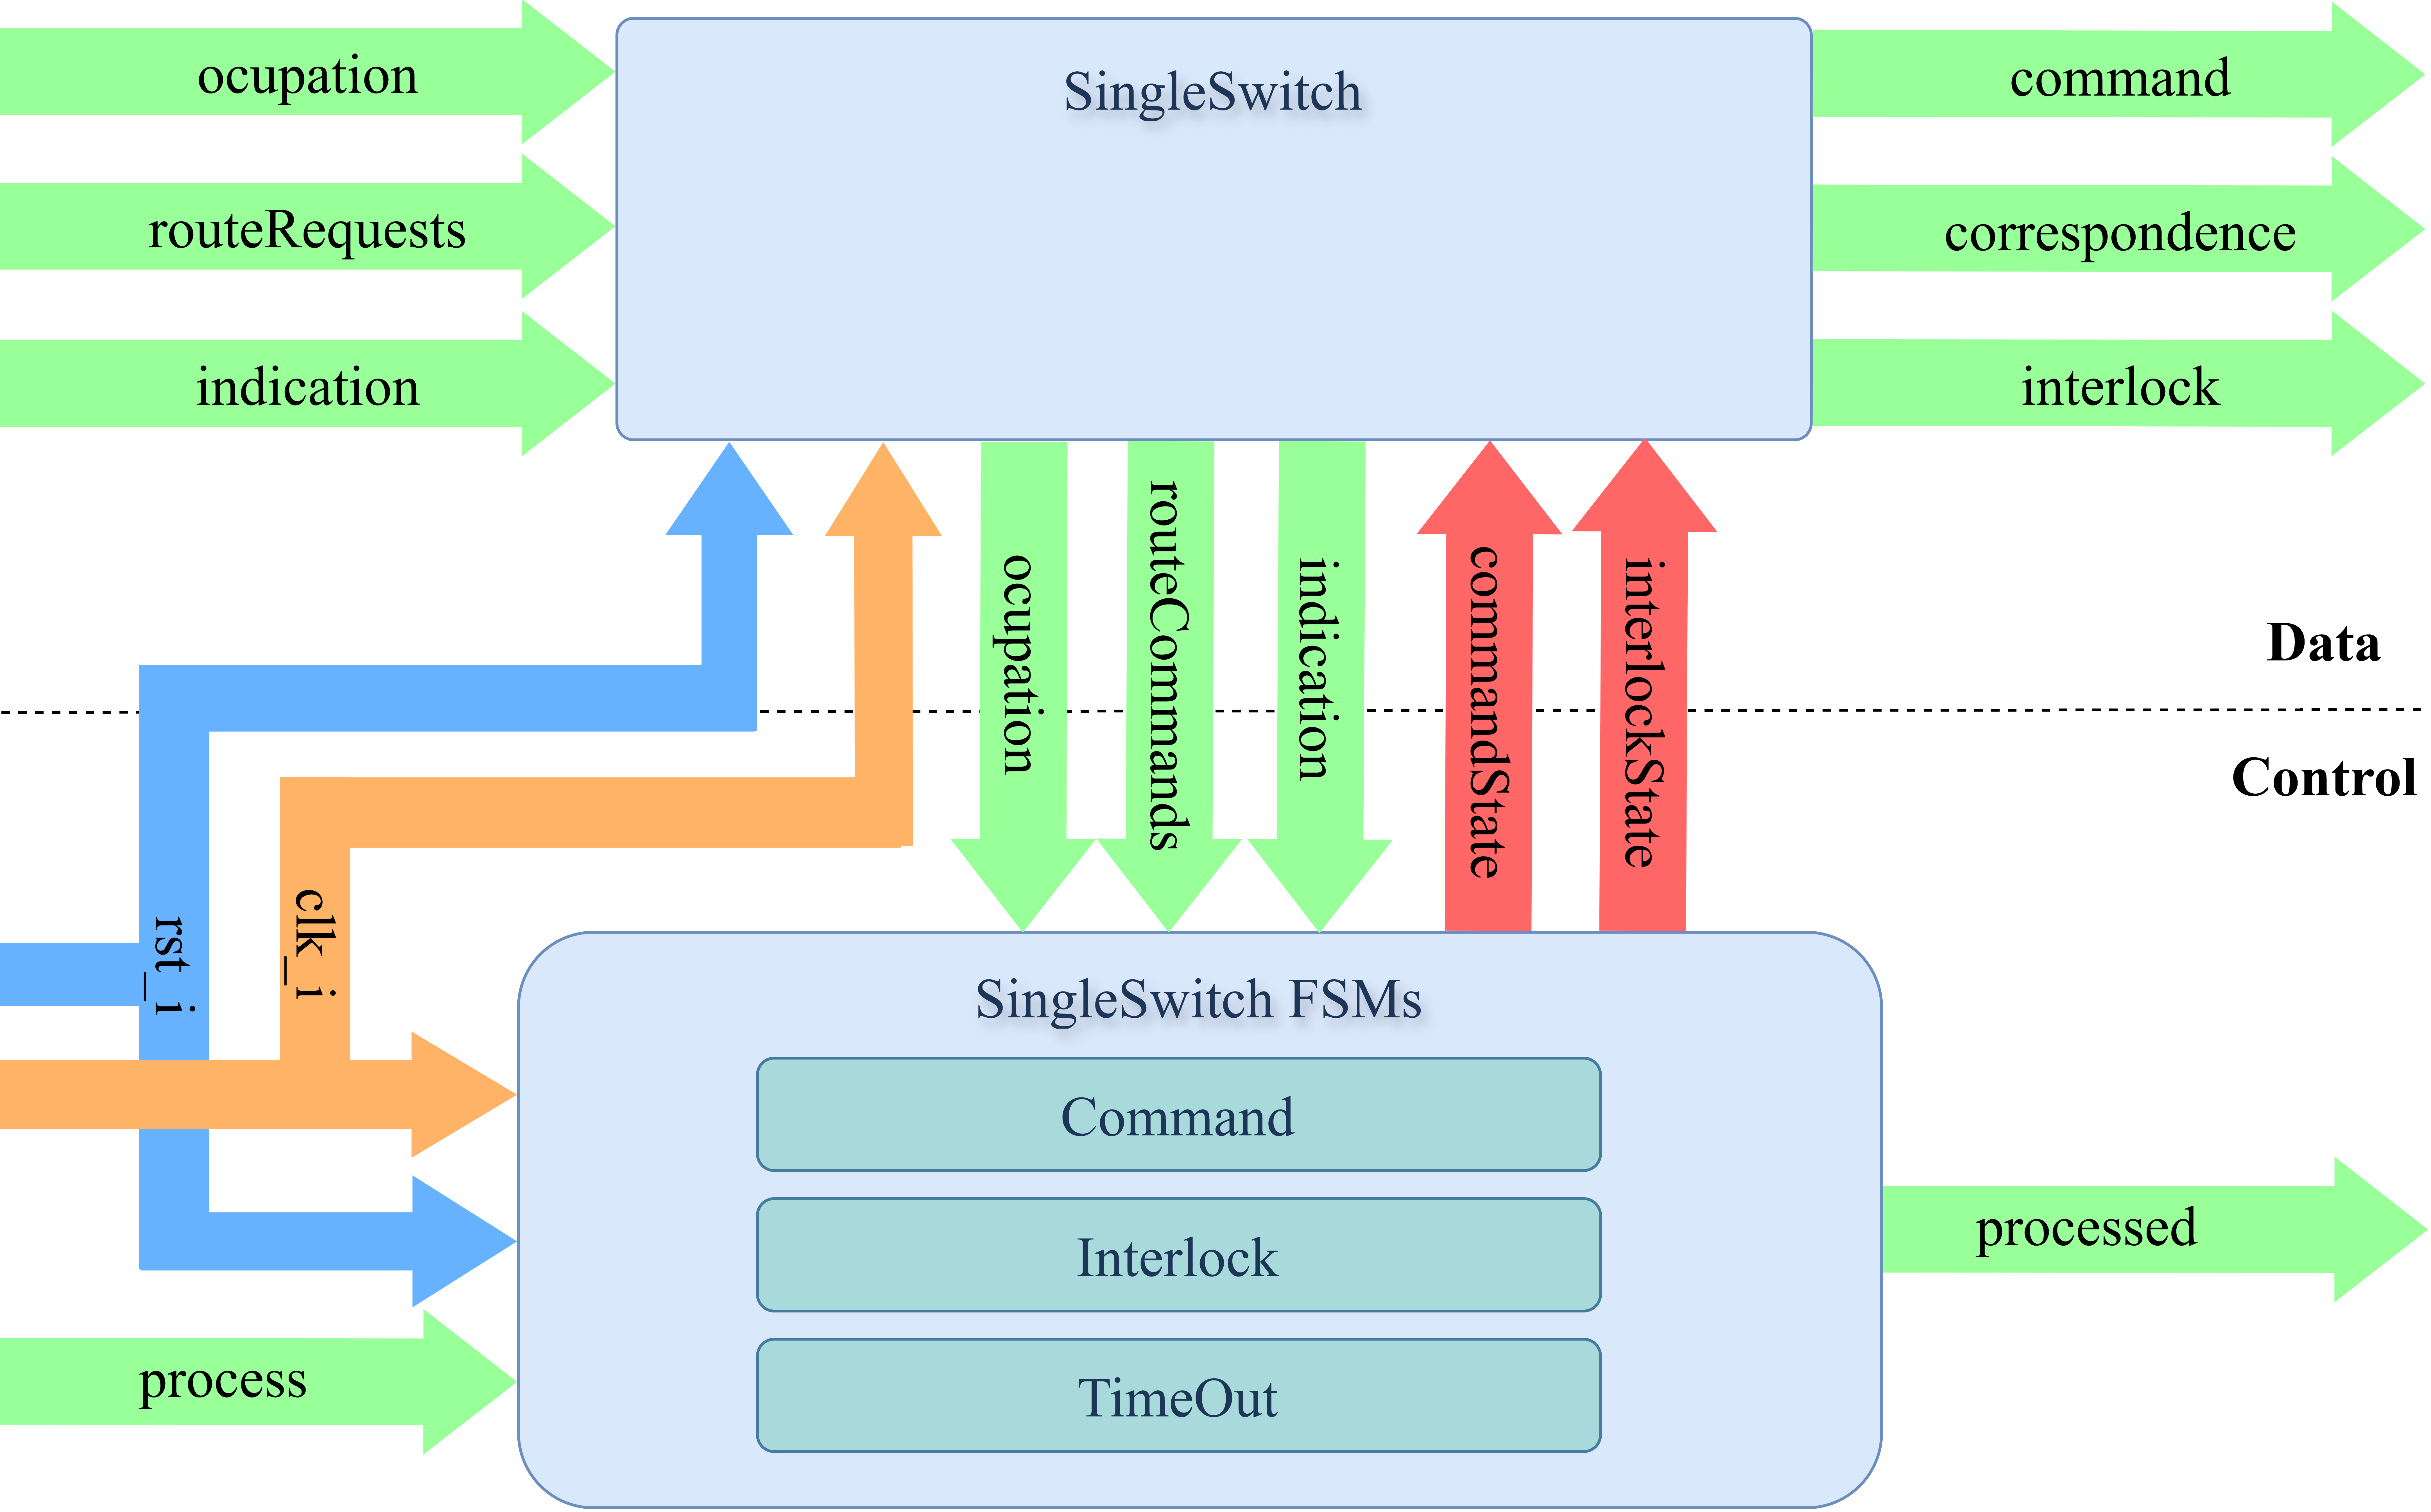
\includegraphics[width=1\textwidth]{Figuras/SSW_module}
		\centering\caption{FSMD del módulo genérico de \textit{SingleSwitches}.}
		\label{fig:SSW_module}
	\end{figure}
	
	Como fue explicado en la Sección \ref{sec:switches}, un cambio de vías simple puede adoptar dos posiciones: normal y reversa. Adicionalmente, es necesario contemplar que mientras la indicación no reporte una posición definida, normal o reverse, se deberá asumir que el cambio de vías se encuentra en transición de un estado al otro. Dicha transición debe ser corta, ya que de no completarse el movimiento puede ser tanto que el cambio de vías se encuentra atascado cómo que el comando o la indicación se encuentren desconectados del actuador. Esta funcionalidad, junto con el comportamiento del cambio de vías genérico se define en la red de Petri de la Figura \ref{fig:SSW_Petri}.
	
	\begin{figure}[H]
		\centering
		\includegraphics[width=1\textwidth]{Figuras/SSW_Petri}
		\centering\caption{Red de Petri del modelo dinámico de \textit{SingleSwitches}.}
		\label{fig:SSW_Petri}
	\end{figure}
	
	Un cambio de vías en estado reversa iniciará su transición si alguna de las rutas envía un comando para modificar la posición a normal, siempre que el cambio de vías no se encuentre enclavado por otra ruta que lo esté utilizando. Durante la transición, salvo que ocurra un timeout, el cambio de vías pasará al estado normal si se confirma la indicación normal y no el comando normal no fue cancelado por la ruta. Análogamente, el cambio de vías puede pasar del estado normal al reversa mediante la secuencia opuesta. Debiendo cumplir las mismas condiciones de no estar enclavado antes de mover el cambio de vías, confirmación de indicación y comando, y realizar todo el proceso dentro de un tiempo determinado.
	
	En el caso del timeout, se considera que si el cambio de vías no reporta una posición final en menos de un tiempo determinado, entonces el cambio de vías debe volver al estado anterior, de ser posible. De lograrse este o no, el cambio de vías igualmente quedará anulado y no podrá ser utilizado por la ruta que lo demanda, prohibiendo la habilitación de dicha ruta.

\subsection{Módulo genérico de los cambios de vías dobles}

\lipsum[1]

\begin{figure}[H]
	\centering
	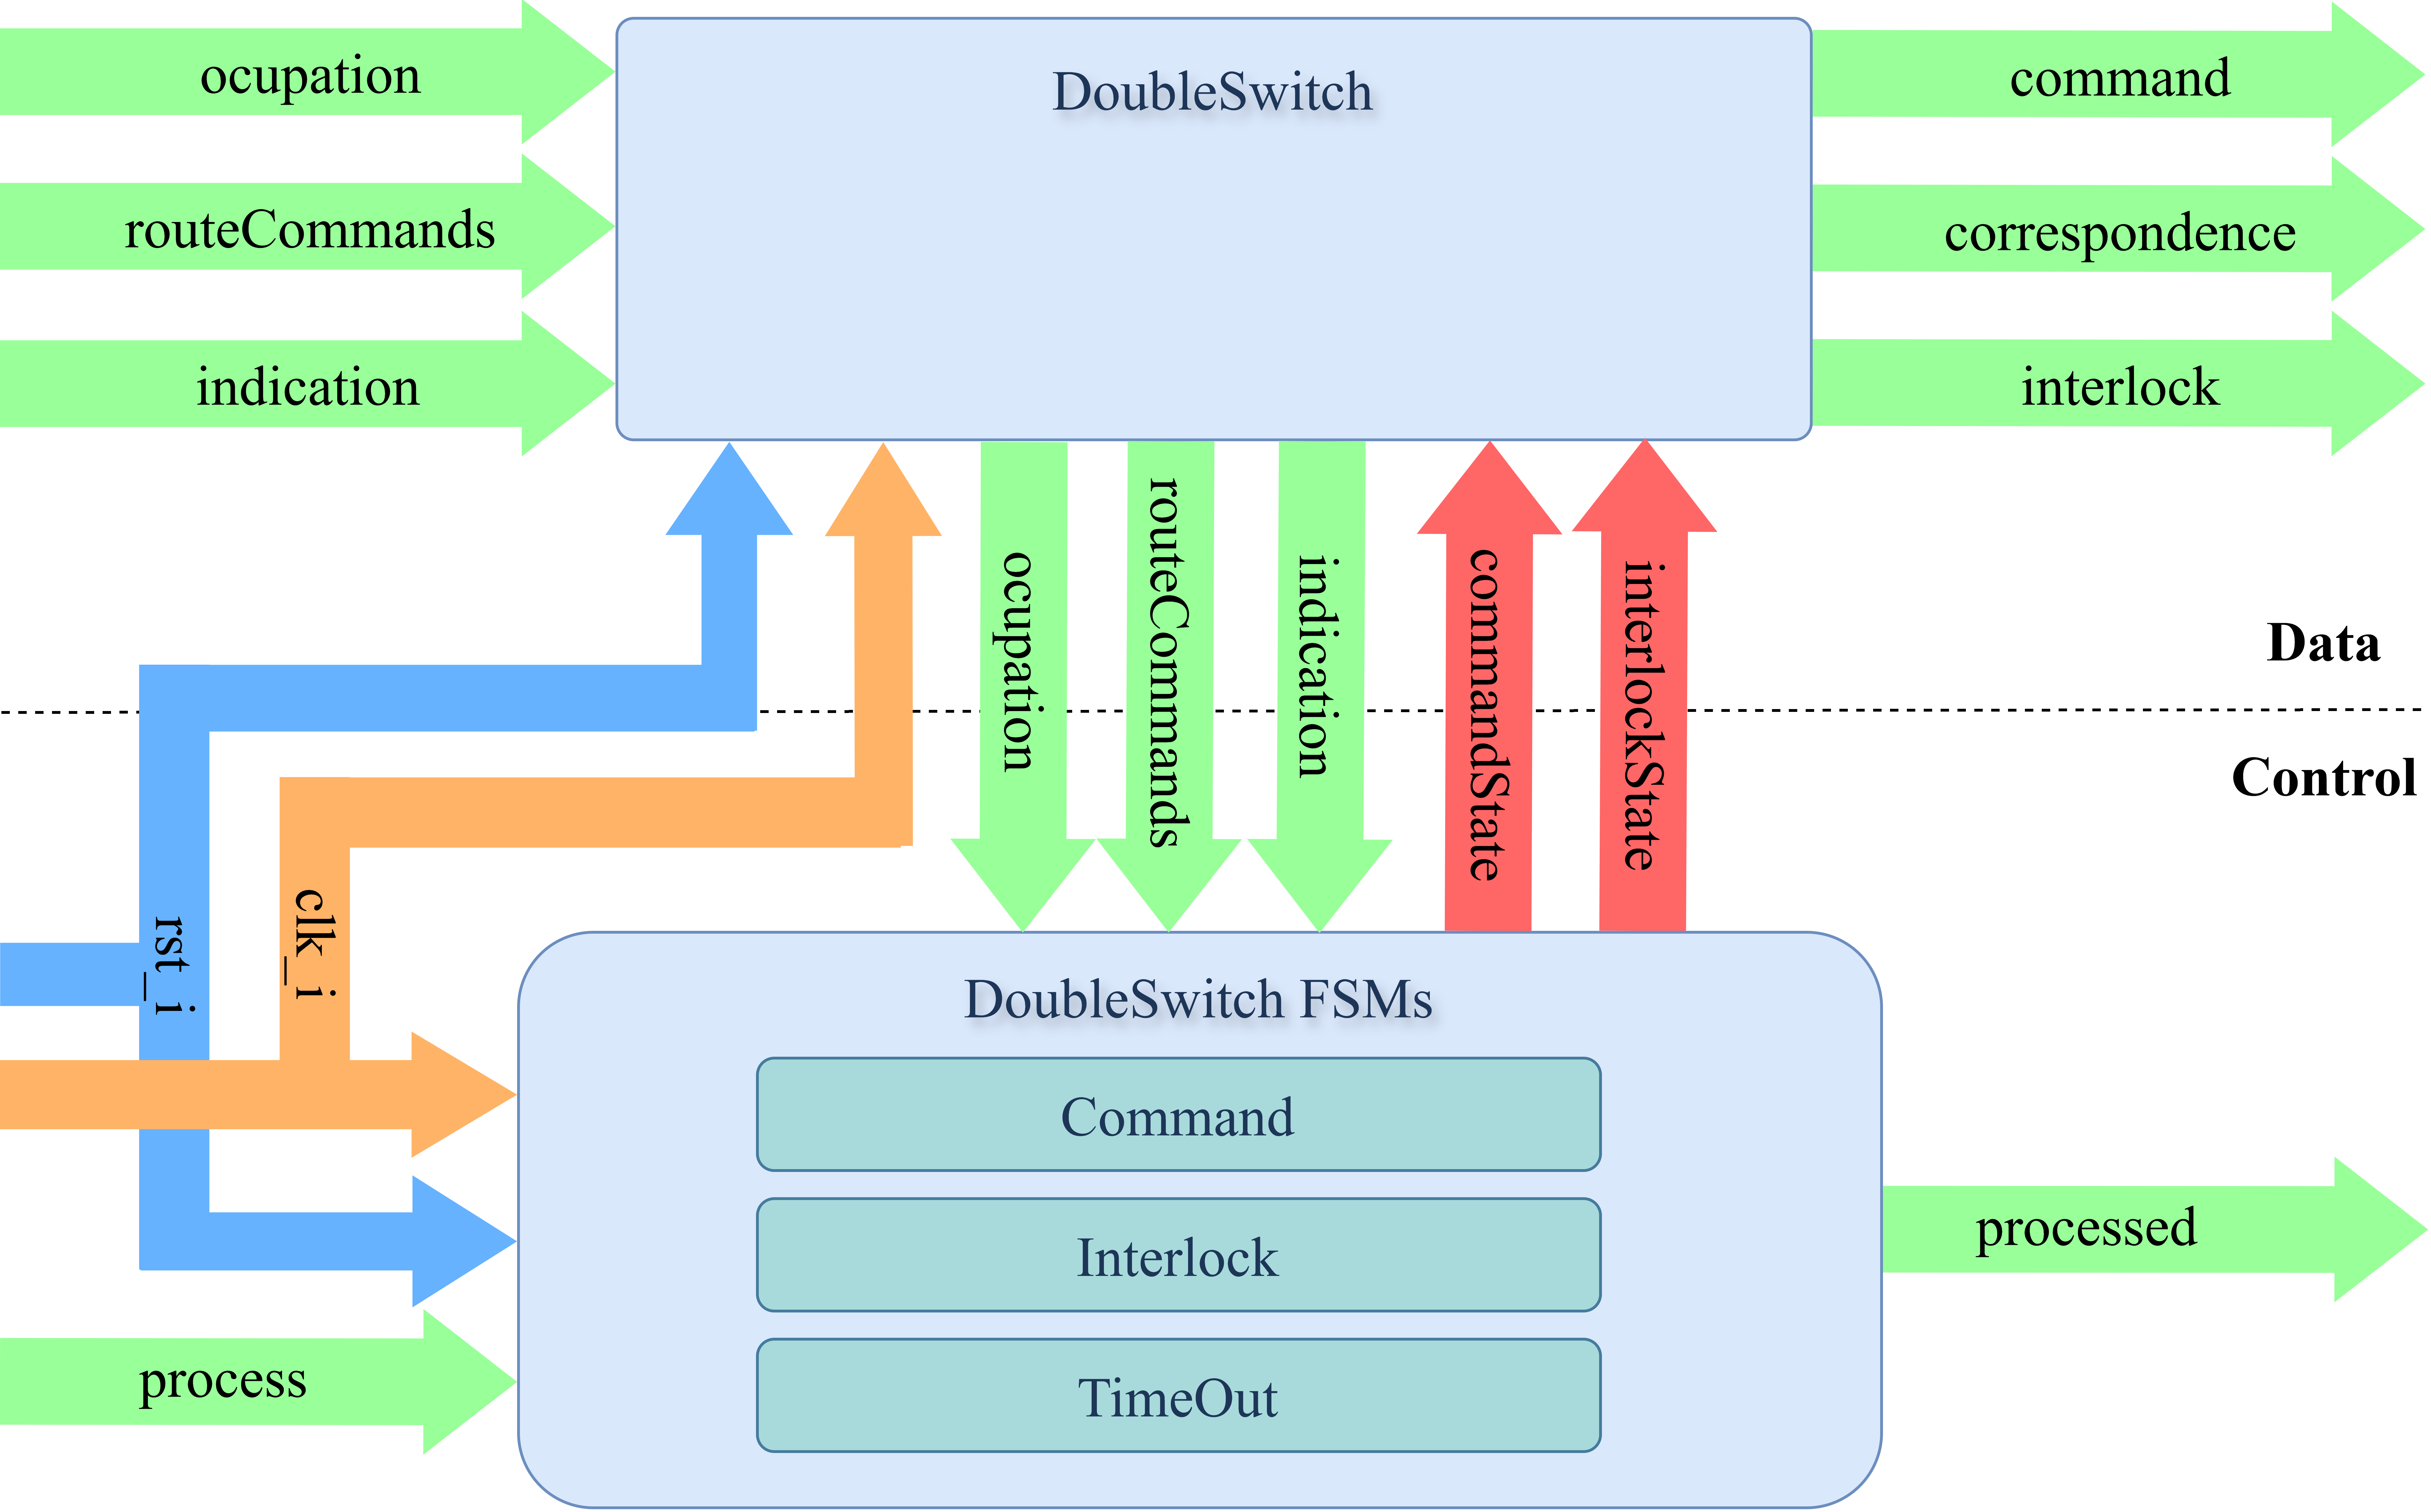
\includegraphics[width=1\textwidth]{Figuras/DSW_module}
	\centering\caption{FSMD del módulo genérico de \textit{DoubleSwitches}.}
	\label{fig:DSW_module}
\end{figure}

\lipsum[1]
\subsection{Módulo genérico de los cambios en tijeras}

\lipsum[1]

\begin{figure}[H]
	\centering
	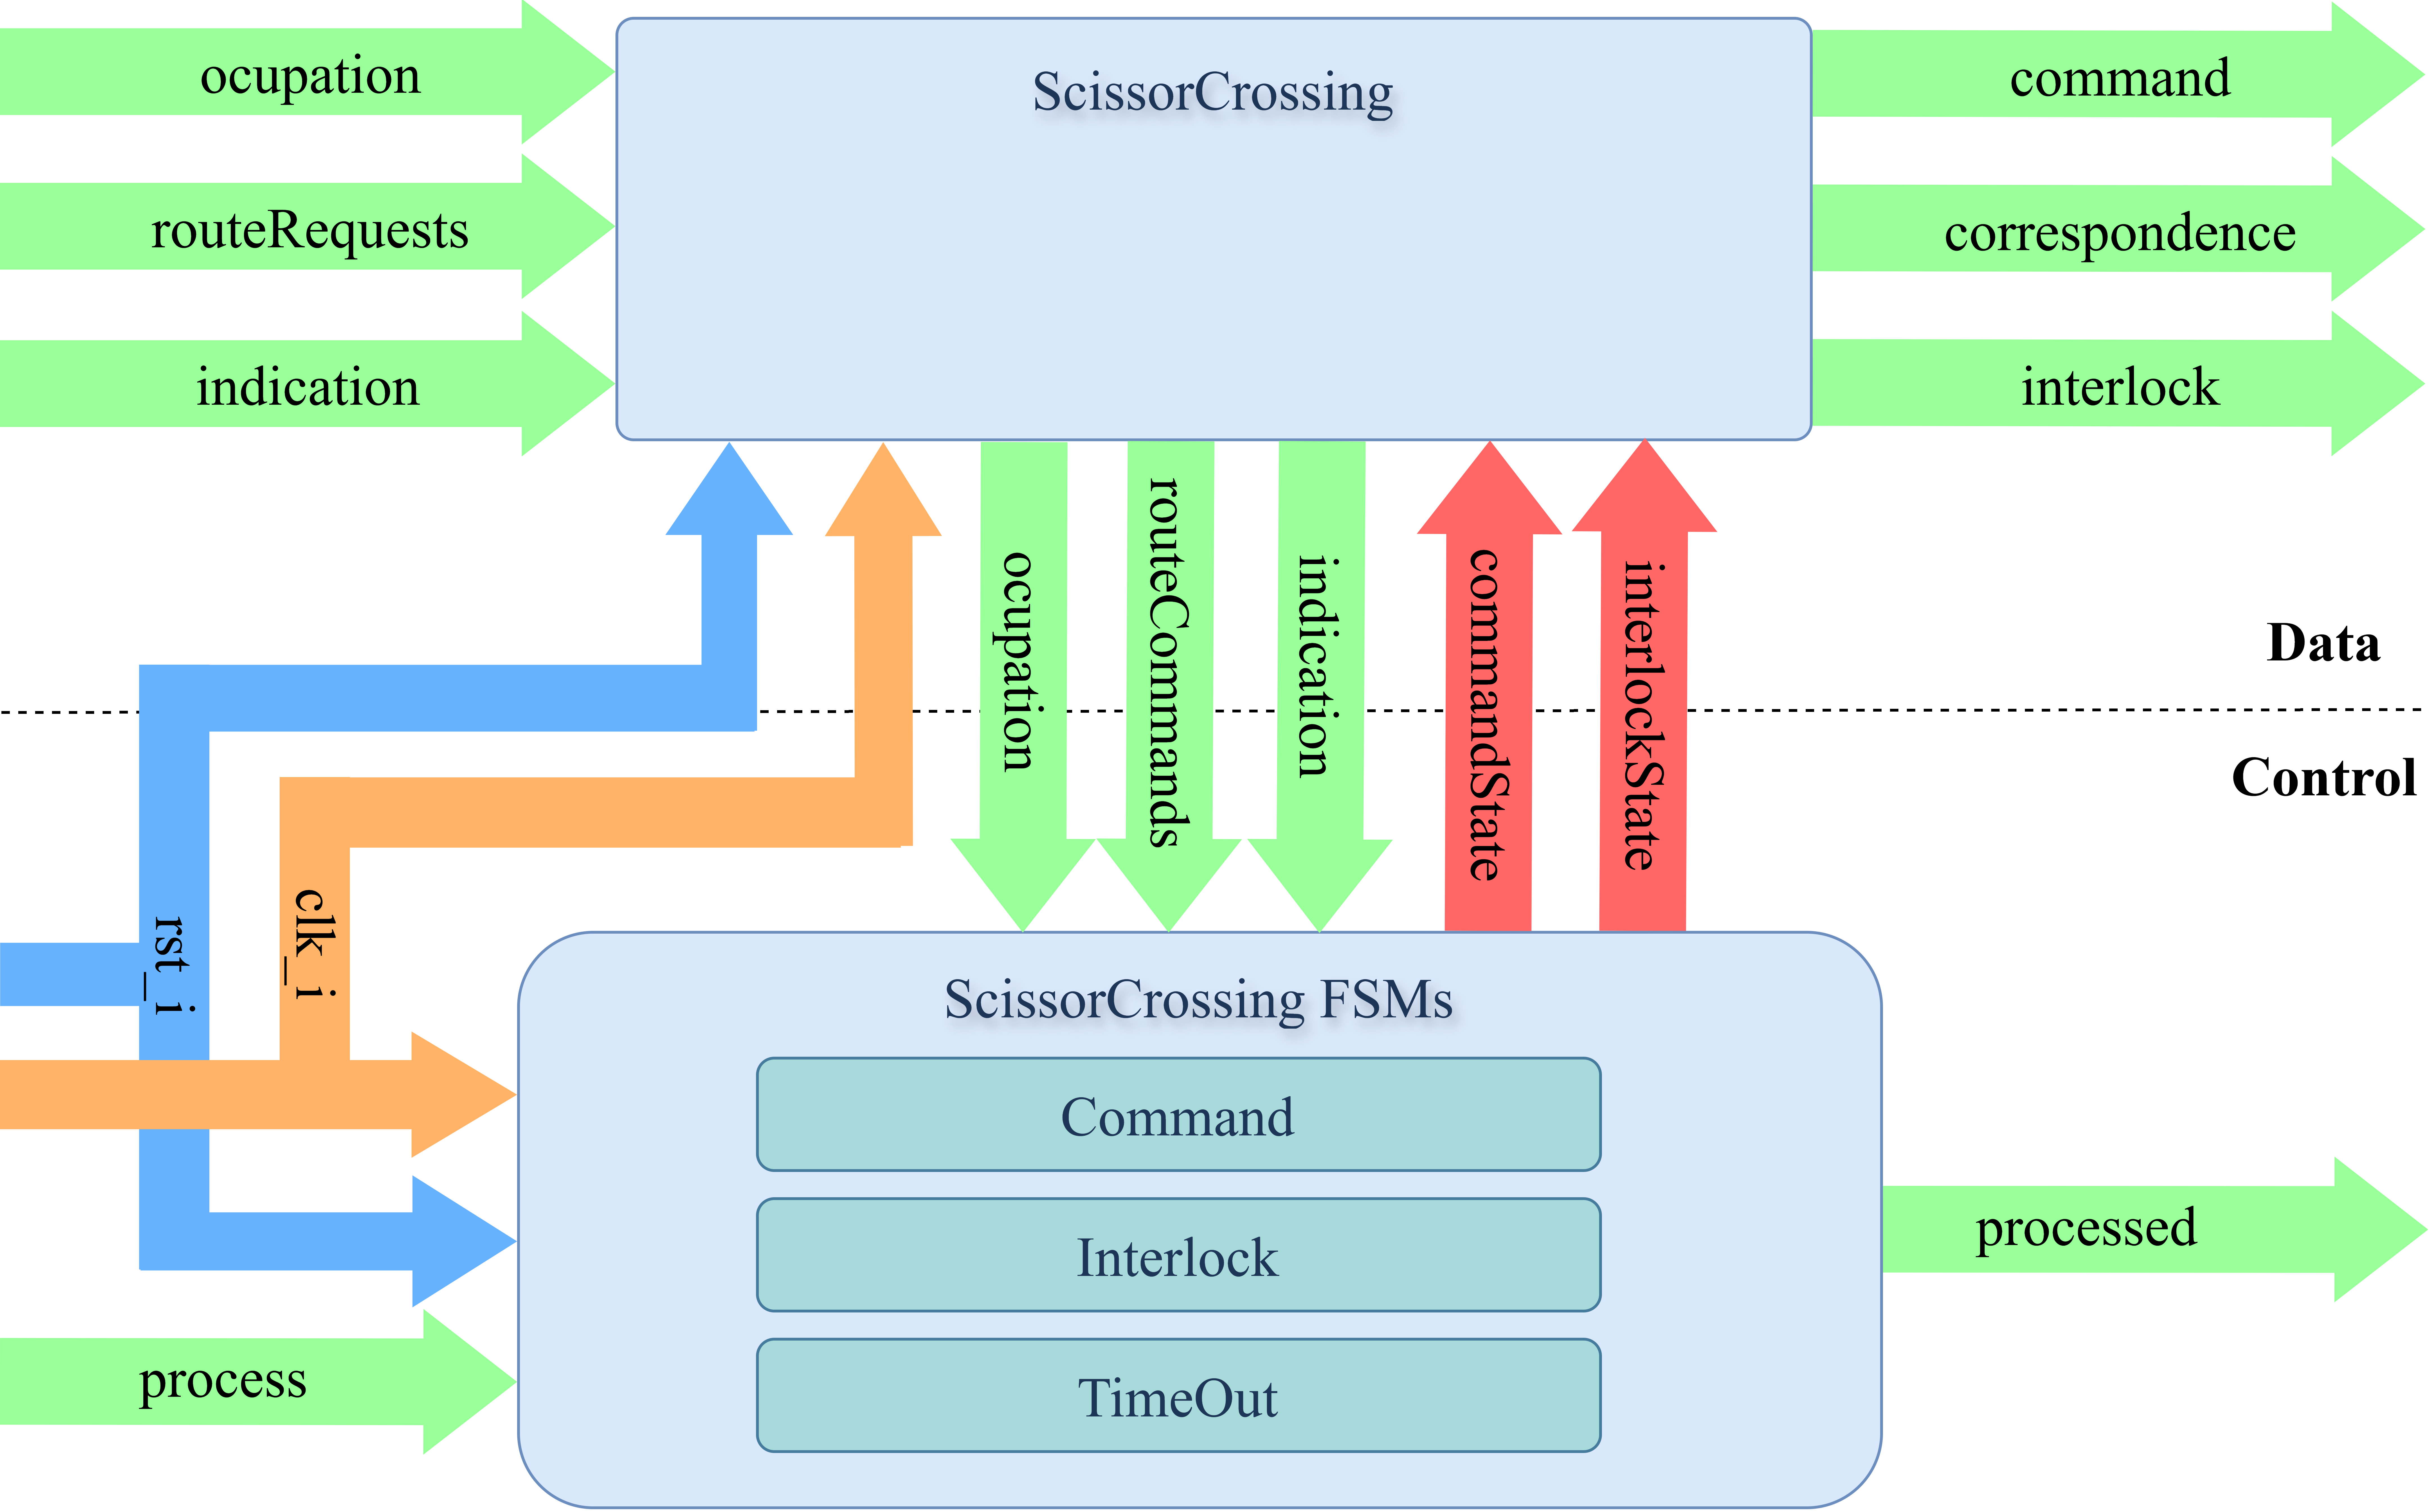
\includegraphics[width=1\textwidth]{Figuras/SCR_module}
	\centering\caption{FSMD del módulo genérico de \textit{ScissorCrossings}.}
	\label{fig:SCR_module}
\end{figure}

\lipsum[1]
\subsection{Módulo genérico de los netElements}

El módulo \textit{NetElements} es el encargado de implementar el reporte del estado de ocupación de las vías. A diferencia de otros módulos centrados en el funcionamiento de mecanismos ferroviarios, leyendo su estado y enviando comandos para operarlo; el módulo de \textit{NetElements} solo se ocupa de reportar estados de sólo lectura, la presencia o no de una formación ferroviaria en una vía determinada, sin poder modificar sus valores de ninguna manera.

El ACG utiliza la información otorgada por el RNA para determinar las entradas y salidas cada módulo \textit{NetElements}, implementando uno por cada \textit{NetElement} definido en la red. Cada uno de estos módulos tendrá sus propios \textit{NetElements} leyendo su estado (\textit{ocupation}) y recibiendo consultas de las rutas que los solicitan (\textit{routeCommands}). A su vez, deberán a las rutas que los utilizan cuál es su estado (ocupado o libre, en el puerto \textit{state}) y si se encuentran enclavados (liberados, reservados o enclavados; en el puerto \textit{interlock}). El diagrama de bloques de las máquinas de estado finitas con camino de datos diseñado para lograr este objetivo se muestra en la Figura \ref{fig:NET_module}.

\begin{figure}[H]
	\centering
	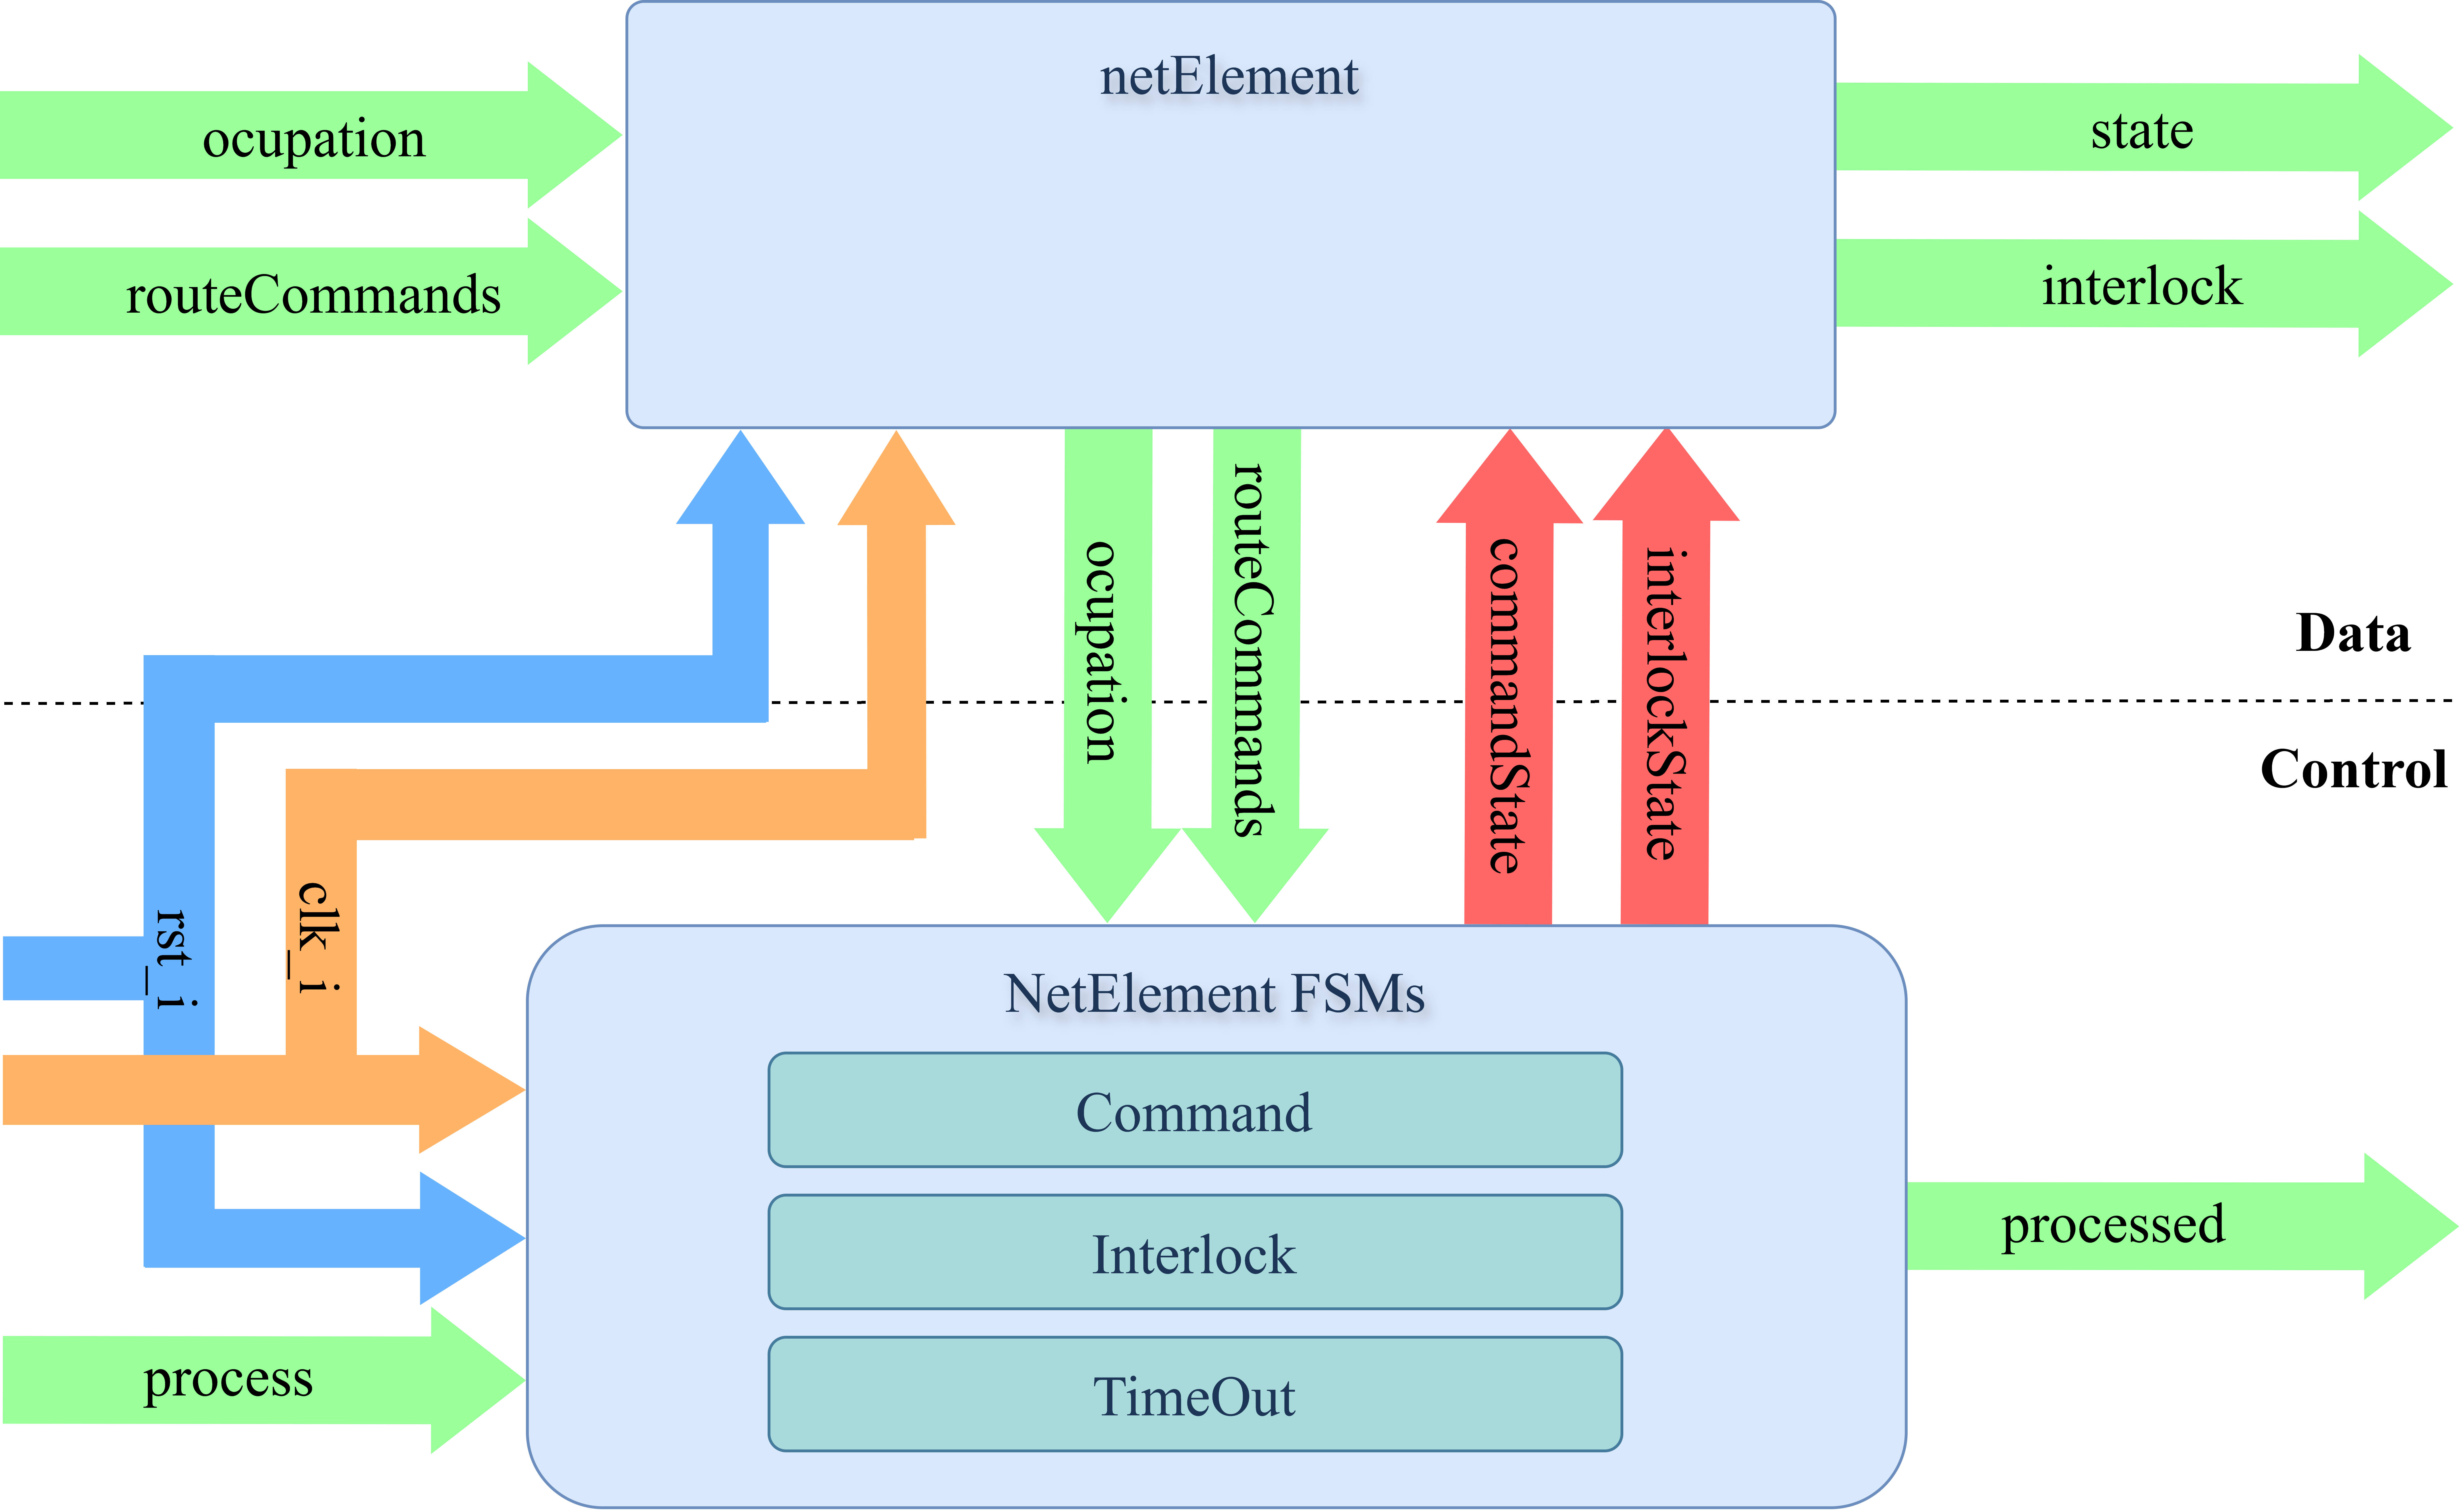
\includegraphics[width=1\textwidth]{Figuras/NET_module}
	\centering\caption{FSMD del módulo genérico de \textit{NetElements}.}
	\label{fig:NET_module}
\end{figure}

Cualquier ruta que pase por sobre el \textit{NetElement} en cuestión puede consultar su estado utilizando el puerto \textit{routeCommands}. Como ya fue explicado en la Sección \ref{sec:detectors}, un circuito de vía asociado a un \textit{netElement} puede estar ocupado por una formación o libre. Todos los módulos \textit{NetElements} reportaran su estado, independientemente si se encuentran reservados o enclavados. La reserva o enclavamiento es meramente para ser utilizado por las rutas para no considerar como propio un \textit{NetElement} que se encuentra libre pero ya ha sido reservado por otra ruta antagónica. El comportamiento del reporte del estado de ocupación de las vías se define en la red de Petri de la Figura \ref{fig:NET_Petri}.

\begin{figure}[H]
	\centering
	\includegraphics[width=0.75\textwidth]{Figuras/NET_Petri}
	\centering\caption{Red de Petri del modelo dinámico de \textit{NetElements}.}
	\label{fig:NET_Petri}
\end{figure}

La simpleza de la implementación del módulo \textit{NetElements} facilita una rápida respuesta por parte del sistema de enclavamientos, al otorgar la información requerida solamente a las rutas que la solicitan, reduciendo enormemente la cantidad de puertos y conexiones a implementar. El ACG creara, además, todas las conexiones necesarias entre cada módulo de elementos ferroviarios y los módulo \textit{NetElements} que los contienen, además de los vecinos mas próximos, para disminuir las chances de que ocurran situaciones peligrosas.
\subsection{Módulo genérico de las señales ferroviarias}
	\label{sec:ACG_sig}
	
	El módulo \textit{Signals} es el encargado de implementar el funcionamiento de las señales ferroviarias. El ACG determine cuantos caminos posibles existen utilizando como punto de partida la señal ferroviaria a implementar. Cada uno de los caminos posibles influirá en el comportamiento de la señal ferroviaria. Para determinar cual es el único camino posible, el ACG implementa los puertos y conexiones a cada uno de los elementos ferroviarios involucrados con esa señal y hasta dos señales futuras, para todos sus caminos. En base a los estados reportados por estos elementos ferroviarios, el módulo \textit{Signals} determinará cuál es el camino activo y su señal ferroviaria quedará definida totalmente. El diagrama de bloques de las máquinas de estado finitas con camino de datos diseñado para lograr este objetivo se muestra en la Figura \ref{fig:SIG_module}.
	
	\begin{figure}[H]
		\centering
		\includegraphics[width=1\textwidth]{Figuras/SIG_module}
		\centering\caption{FSMD del módulo genérico de \textit{Signals}.}
		\label{fig:SIG_module}
	\end{figure}
	
	Como fue explicado en la Sección XXX, el aspecto de una señal ferroviaria será rojo si el conjunto de \textit{netElements} al que habilita circular la formación ferroviaria se encuentra ocupado. Si se encontrasen desocupados, su aspecto dependerá del aspecto de la señal siguiente. Pero cuál es la señal siguiente dependerá del estado actual de toda la infraestructura entre la señal analizada y dos señales consecutivas. El comportamiento del aspecto de una señal ferroviaria se define en la red de Petri de la Figura \ref{fig:SIG_Petri}.
	
	\begin{figure}[H]
		\centering
		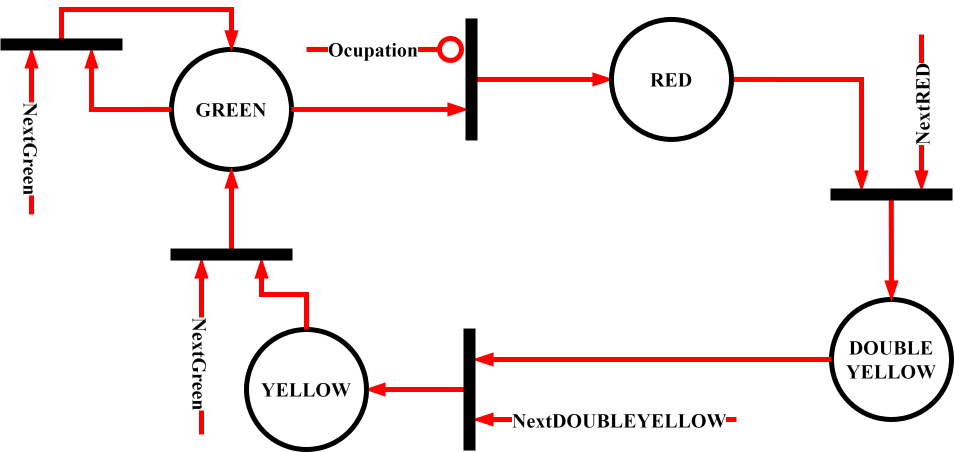
\includegraphics[width=1\textwidth]{Figuras/SIG_petri}
		\centering\caption{Red de Petri del modelo dinámico de \textit{Signals}.}
		\label{fig:SIG_Petri}
	\end{figure}
	
	La red de Petri ilustrada en la Figura \ref{fig:SIG_Petri} es una simplificación de la implementación real, solamente se ilustra un único cambio de estado entre un aspecto y otro. De haber ilustrado todas las transiciones entre, por ejemplo, el aspecto rojo y amarillo, el aspecto rojo y verde, o el aspecto rojo consigo mismo, entonces la cantidad de transiciones sería tres veces mayor.
	
	Teniendo en cuenta el modelo simplificado, una señal ferroviaria depende de si misma solo si la sección a la que protege se encuentra ocupada, en cuyo caso su aspecto será rojo. En caso contrario, si la sección se encuentra libre, dependerá del aspecto de la señal siguiente: si la señal siguiente es roja, el aspecto de la señal analizada será doble amarillo; si la señal siguiente es doble amarilla, el aspecto de la señal analizada será amarillo; si la señal siguiente es amarilla, el aspecto de la señal analizada será verde y, finalmente, si la señal siguiente es verde, el aspecto de la señal analizada también lo será.
	
	Las señales ferroviarias no pueden cambiar su aspecto una vez que se encuentran enclavadas, salvo para adoptar un aspecto mas restrictivo, para garantizar un mayor nivel de seguridad.
\subsection{Módulo genérico de las rutas ferroviarias}

\lipsum[1]

\begin{figure}[H]
	\centering
	\includegraphics[width=1\textwidth]{Figuras/RTS_module}
	\centering\caption{FSMD del módulo genérico de \textit{Routes}}
	\label{fig:RTS_module}
\end{figure}

\lipsum[1]    
    \section{Redundancia}

\lipsum[1]

\begin{figure}[!h]
        \centering
        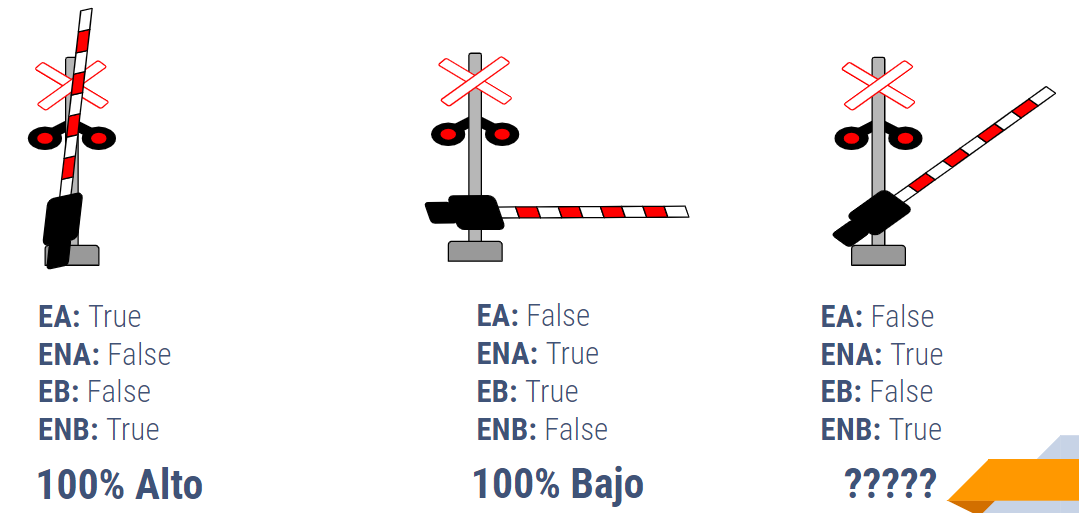
\includegraphics[width=1\textwidth]{Figuras/antagonica}
        \centering\caption{XXXXX.}
        \label{fig:redundancia_1}
    \end{figure}

\lipsum[1]

    \section{Validacion de la implementacion}

\lipsum[1]